\documentclass[twoside]{book}

% Packages required by doxygen
\usepackage{fixltx2e}
\usepackage{calc}
\usepackage{doxygen}
\usepackage[export]{adjustbox} % also loads graphicx
\usepackage{graphicx}
\usepackage[utf8]{inputenc}
\usepackage{makeidx}
\usepackage{multicol}
\usepackage{multirow}
\PassOptionsToPackage{warn}{textcomp}
\usepackage{textcomp}
\usepackage[nointegrals]{wasysym}
\usepackage[table]{xcolor}

% Font selection
\usepackage[T1]{fontenc}
\usepackage[scaled=.90]{helvet}
\usepackage{courier}
\usepackage{amssymb}
\usepackage{sectsty}
\renewcommand{\familydefault}{\sfdefault}
\allsectionsfont{%
  \fontseries{bc}\selectfont%
  \color{darkgray}%
}
\renewcommand{\DoxyLabelFont}{%
  \fontseries{bc}\selectfont%
  \color{darkgray}%
}
\newcommand{\+}{\discretionary{\mbox{\scriptsize$\hookleftarrow$}}{}{}}

% Page & text layout
\usepackage{geometry}
\geometry{%
  a4paper,%
  top=2.5cm,%
  bottom=2.5cm,%
  left=2.5cm,%
  right=2.5cm%
}
\tolerance=750
\hfuzz=15pt
\hbadness=750
\setlength{\emergencystretch}{15pt}
\setlength{\parindent}{0cm}
\setlength{\parskip}{3ex plus 2ex minus 2ex}
\makeatletter
\renewcommand{\paragraph}{%
  \@startsection{paragraph}{4}{0ex}{-1.0ex}{1.0ex}{%
    \normalfont\normalsize\bfseries\SS@parafont%
  }%
}
\renewcommand{\subparagraph}{%
  \@startsection{subparagraph}{5}{0ex}{-1.0ex}{1.0ex}{%
    \normalfont\normalsize\bfseries\SS@subparafont%
  }%
}
\makeatother

% Headers & footers
\usepackage{fancyhdr}
\pagestyle{fancyplain}
\fancyhead[LE]{\fancyplain{}{\bfseries\thepage}}
\fancyhead[CE]{\fancyplain{}{}}
\fancyhead[RE]{\fancyplain{}{\bfseries\leftmark}}
\fancyhead[LO]{\fancyplain{}{\bfseries\rightmark}}
\fancyhead[CO]{\fancyplain{}{}}
\fancyhead[RO]{\fancyplain{}{\bfseries\thepage}}
\fancyfoot[LE]{\fancyplain{}{}}
\fancyfoot[CE]{\fancyplain{}{}}
\fancyfoot[RE]{\fancyplain{}{\bfseries\scriptsize Generated by Doxygen }}
\fancyfoot[LO]{\fancyplain{}{\bfseries\scriptsize Generated by Doxygen }}
\fancyfoot[CO]{\fancyplain{}{}}
\fancyfoot[RO]{\fancyplain{}{}}
\renewcommand{\footrulewidth}{0.4pt}
\renewcommand{\chaptermark}[1]{%
  \markboth{#1}{}%
}
\renewcommand{\sectionmark}[1]{%
  \markright{\thesection\ #1}%
}

% Indices & bibliography
\usepackage{natbib}
\usepackage[titles]{tocloft}
\setcounter{tocdepth}{3}
\setcounter{secnumdepth}{5}
\makeindex

% Hyperlinks (required, but should be loaded last)
\usepackage{ifpdf}
\ifpdf
  \usepackage[pdftex,pagebackref=true]{hyperref}
\else
  \usepackage[ps2pdf,pagebackref=true]{hyperref}
\fi
\hypersetup{%
  colorlinks=true,%
  linkcolor=blue,%
  citecolor=blue,%
  unicode%
}

% Custom commands
\newcommand{\clearemptydoublepage}{%
  \newpage{\pagestyle{empty}\cleardoublepage}%
}

\usepackage{caption}
\captionsetup{labelsep=space,justification=centering,font={bf},singlelinecheck=off,skip=4pt,position=top}

%===== C O N T E N T S =====

\begin{document}

% Titlepage & ToC
\hypersetup{pageanchor=false,
             bookmarksnumbered=true,
             pdfencoding=unicode
            }
\pagenumbering{alph}
\begin{titlepage}
\vspace*{7cm}
\begin{center}%
{\Large Iteration 3 Documentation }\\
\vspace*{1cm}
{\large Generated by Doxygen 1.8.14}\\
\end{center}
\end{titlepage}
\clearemptydoublepage
\pagenumbering{roman}
\tableofcontents
\clearemptydoublepage
\pagenumbering{arabic}
\hypersetup{pageanchor=true}

%--- Begin generated contents ---
\chapter{Iteration 3 Documentation}
\label{index}\hypertarget{index}{}\hypertarget{index_intro_sec}{}\section{Technical Introduction}\label{index_intro_sec}
This program creates a robot simulation, in which an autonomous robot moves around a 2D world. The robot moves based upon it’s behavior and hunger level. This software is written in C++, making the use of the Open\+GL graphics library, as well as the nanogui library. Compilation requires the installation of the Min\+Gfx library. This library creates the 2D graphics window that the arena lives in and animates both the entities and the environment using a continuous control loop.\hypertarget{index_mvc_sec}{}\section{Model-\/\+View-\/\+Controller}\label{index_mvc_sec}
This software follows the model-\/view-\/ controller(\+M\+V\+C) design pattern, which corresponds to three primary classes where the bulk of the code is held in\+: \mbox{\hyperlink{class_arena}{Arena}}, \mbox{\hyperlink{class_graphics_arena_viewer}{Graphics\+Arena\+Viewer}}, and \mbox{\hyperlink{class_controller}{Controller}}.

The Model in this implementation is the \mbox{\hyperlink{class_arena}{Arena}} class. The \mbox{\hyperlink{class_arena}{Arena}} manages all of the entities and their actions. For instance, methods that perform tasks such as removing and adding entities to the simulation are defined here, methods for controlling the movement are defined to some degree here, and there is a substantial method, Update\+Entities\+Timestep, which calculates the proper positioning and action after each time step. A time step in this context is an iteration through the game loop.

The \mbox{\hyperlink{class_graphics_arena_viewer}{Graphics\+Arena\+Viewer}} handles both user input and graphical display of the simulation. This is the part of the project which relies on the Min\+Gfx library mentioned earlier as it inherits from the Min\+Gfx class Graphics\+App. The \mbox{\hyperlink{class_graphics_arena_viewer}{Graphics\+Arena\+Viewer}} controls the timing of the simulation and the graphics display by using a loop that calls Update\+Simulation and Draw\+Using\+Nano\+VG at each iteration.

The \mbox{\hyperlink{class_controller}{Controller}} class is the last of the three classes that is influenced by the M\+VC design pattern. This class acts as a connection between the \mbox{\hyperlink{class_graphics_arena_viewer}{Graphics\+Arena\+Viewer}} and the \mbox{\hyperlink{class_arena}{Arena}}. For example, if a user were to add a robot to the simulation they would alter the slider in the \mbox{\hyperlink{class_graphics_arena_viewer}{Graphics\+Arena\+Viewer}} which would in turn call a method of the controller class, which then would decide what method is best to call in the \mbox{\hyperlink{class_arena}{Arena}} class.\hypertarget{index_entities_sec}{}\section{Entities}\label{index_entities_sec}
As mentioned previously there are multiple entities that exist within the simulation. The three entities are as follows\+: \mbox{\hyperlink{class_robot}{Robot}}, \mbox{\hyperlink{class_light}{Light}}, and \mbox{\hyperlink{class_food}{Food}}.

\mbox{\hyperlink{class_robot}{Robot}} is the main entity in the simulation. The robot autonomously moves based on two attributes\+: hunger level and behavior. If there is food in the arena that robot has a hunger level. The hunger level, which is based on a timer, is defined to be decremented within the robot’s Timestep\+Update method. This implementation of the software uses the dt or delta time to control the hunger timer and not the computer clock. Due to this implementation runtime fluctuates slightly between machines however the total time from no hunger to starvation is $\sim$2 minutes and 30 seconds. The robot’s \mbox{\hyperlink{class_food}{Food}} \mbox{\hyperlink{class_sensor}{Sensor}} which inherits from a parent \mbox{\hyperlink{class_sensor}{Sensor}} class guides the robot towards the location of a \mbox{\hyperlink{class_food}{Food}} entity. Based upon the hunger stage the robot is either only influenced by light, influenced by light and food, or only influenced by food. The other way the robot moves is in response to the light entities. The robot can have one of two behaviors\+: \mbox{\hyperlink{class_fear}{Fear}} or \mbox{\hyperlink{class_explore}{Explore}}. The \mbox{\hyperlink{class_fear}{Fear}} behavior makes the robot moves slow away from the light and move away quickly when it comes towards the light and the \mbox{\hyperlink{class_explore}{Explore}} behavior moves quickly when not near the light and moves away slowly when near the light in an effort to avoid them. The robot controls the response to lights by using its \mbox{\hyperlink{class_light}{Light}} \mbox{\hyperlink{class_sensor}{Sensor}} which much like the \mbox{\hyperlink{class_food}{Food}} \mbox{\hyperlink{class_sensor}{Sensor}} inherits from the same parent \mbox{\hyperlink{class_sensor}{Sensor}} class.

The Robot’s movement is handled using a combination of differential drive and Sensors. Differential drive is the concept that the robot has two wheels and it turns when one wheel has a higher velocity than another. Both Sensors act similarly just with different stimuli. The robot has two sensors placed 40 degrees away from its main focal point. With each time step, a Notify method notifying the sensor of its respective entities is called. This implementation is based on the Observer Pattern. The Notify method (which is a virtual method of the \mbox{\hyperlink{class_sensor}{Sensor}} class is overwritten within in both the \mbox{\hyperlink{class_food}{Food}} and the \mbox{\hyperlink{class_light}{Light}} \mbox{\hyperlink{class_sensor}{Sensor}} classes) calculates sensor readings based upon the robot’s distance from other entities. The function used to do this is as follows\+: reading = 1200/(distance$^\wedge$1.08). This reading is then passed into an Update\+Velocity method which is part of the \mbox{\hyperlink{class_motion_handler_robot}{Motion\+Handler\+Robot}} class. In the \mbox{\hyperlink{class_motion_handler_robot}{Motion\+Handler\+Robot}} the Strategy design pattern is used to control the type of robot (fear or explore). This done by having a \mbox{\hyperlink{class_braitenberg}{Braitenberg}} parent class as an attribute and defining the behavior at runtime. The Update\+Velocity method is defined according to the type of the robot. The definitions for these can be seen in their respective definition is \mbox{\hyperlink{fear_8cc}{fear.\+cc}} and \mbox{\hyperlink{explore_8cc}{explore.\+cc}}. Please note that there is an aggressive behavior for the food as well that is only used when the robot is starving.

The \mbox{\hyperlink{class_light}{Light}} is the second entity. Lights move in a static fashion. They always move straight until they collide with a wall, at that point they move in an arc back in order to avoid never ending collisions. The Lights collide with walls and other Lights which is shown in the Arena’s Handle\+Entity\+Collision method. The amount of Lights is handled by the sliders in the \mbox{\hyperlink{class_graphics_arena_viewer}{Graphics\+Arena\+Viewer}}.

The \mbox{\hyperlink{class_food}{Food}} is the last entity in the simulation. The \mbox{\hyperlink{class_food}{Food}} has no movement at all and is placed randomly within the arena. The robots consume food to reset their hunger level. There is a slider for food as well. If the slider is set to 0 the robot hunger will be shut off using a Boolean attribute of the robot class called has\+\_\+hunger\+\_\+. This attribute will be set to false and the hunger time will not be a factor if the arena has no food.\hypertarget{index_general_sec}{}\section{General Introduction}\label{index_general_sec}
This robot simulations is used to exhibit the reaction of different types of robots to lights. The robots have a behavior, either fear or explore, and a hunger level. Robots also react to food in different ways depending on the hunger level.\hypertarget{index_gui_sec}{}\section{Graphical User Interface (\+G\+U\+I)}\label{index_gui_sec}
The simulation is laid out in a simple fashion. In the far right of the screen there is a toggle menu. At the top of the menu there is a Play/\+Pause button. This button starts and stops the simulation much like a pause button on a video game. This is set to a default value of paused so Play must be pushed each time a new simulation is made. The button beneath it is a New Game button which resets the simulation by resetting all hunger levels and entity positions. Beneath that is an assortment of sliders to control various attributes of the simulation. In order they are\+: Number of \mbox{\hyperlink{class_fear}{Fear}} Robots, Number of \mbox{\hyperlink{class_explore}{Explore}} Robots, Number of Lights, Number of \mbox{\hyperlink{class_food}{Food}}, and Sensitivity of the \mbox{\hyperlink{class_sensor}{Sensor}}. All of these are self-\/explanatory as far as their actions, aside from the sensitivity slider. The lower the sensitivity the less the robots will react to other stimuli. If this is set to zero the robots will move in their default behavior (\mbox{\hyperlink{class_fear}{Fear}} robots will freeze, \mbox{\hyperlink{class_explore}{Explore}} robots will move at maximum velocity) \mbox{[}Please see the next section for descriptions of these behaviors\mbox{]}.

The arena itself is held within the white outline seen on the screen. These white outlines act as the wall or boundaries of the simulation and none of the entities can spawn or move outside of them. The three entities -\/ \mbox{\hyperlink{class_robot}{Robot}}, \mbox{\hyperlink{class_food}{Food}}, \mbox{\hyperlink{class_light}{Light}} – are colored in blue, red, and white respectively. The two dots seen on the robot are its sensor, which will be explained in further detail in the next section. The robots and lights are randomly sized within a certain range while the food is always the same size.\hypertarget{index_how_it_works_sec}{}\section{How the Simulation Works}\label{index_how_it_works_sec}
The robots move autonomously based upon the behavior they exhibit and their hunger level. There are three stages of hunger\+: full (first 30 seconds), hungry (between 30 seconds and 2 minutes), and starving (between 2 minutes and 2 minutes and 30 seconds). Depending on which stage the robot is in it will react in different ways. If it is not hungry it will only react to the lights, if it is hungry it will react to lights and go towards food and if it is starving it will move only towards food and not to lights. If the robot goes 2 minutes and 30 seconds without consuming food the simulation will end and a “\+Y\+OU L\+O\+S\+T” message will appear in the middle of the G\+UI. At that point the New Game button can be pressed to restart.

The other way the robot moves is through its behavior. Robots can have two behaviors, \mbox{\hyperlink{class_fear}{Fear}} or \mbox{\hyperlink{class_explore}{Explore}}. The \mbox{\hyperlink{class_fear}{Fear}} behavior moves slowly away from lights and moves quickly away when coming close to lights. The \mbox{\hyperlink{class_explore}{Explore}} robot moves quickly in a straight line when away from lights and slowly turns away when close to lights.

Collisions are handled in multiple ways depending on the entity. Robots collide with other robots and the wall. Lights collide with other lights and the wall. None of the entities collide with food (food obviously does not handle any collisions as it is immobile). Every entity reverses in an arc when it registers a proper collision. 
\chapter{Hierarchical Index}
\section{Class Hierarchy}
This inheritance list is sorted roughly, but not completely, alphabetically\+:\begin{DoxyCompactList}
\item \contentsline{section}{Arena}{\pageref{class_arena}}{}
\item \contentsline{section}{arena\+\_\+params}{\pageref{structarena__params}}{}
\item \contentsline{section}{Arena\+Entity}{\pageref{class_arena_entity}}{}
\begin{DoxyCompactList}
\item \contentsline{section}{Arena\+Immobile\+Entity}{\pageref{class_arena_immobile_entity}}{}
\begin{DoxyCompactList}
\item \contentsline{section}{Food}{\pageref{class_food}}{}
\end{DoxyCompactList}
\item \contentsline{section}{Arena\+Mobile\+Entity}{\pageref{class_arena_mobile_entity}}{}
\begin{DoxyCompactList}
\item \contentsline{section}{Light}{\pageref{class_light}}{}
\item \contentsline{section}{Robot}{\pageref{class_robot}}{}
\end{DoxyCompactList}
\end{DoxyCompactList}
\item \contentsline{section}{Braitenberg}{\pageref{class_braitenberg}}{}
\begin{DoxyCompactList}
\item \contentsline{section}{Aggression}{\pageref{class_aggression}}{}
\item \contentsline{section}{Explore}{\pageref{class_explore}}{}
\item \contentsline{section}{Fear}{\pageref{class_fear}}{}
\end{DoxyCompactList}
\item \contentsline{section}{Controller}{\pageref{class_controller}}{}
\item \contentsline{section}{Entity\+Factory}{\pageref{class_entity_factory}}{}
\item Graphics\+App\begin{DoxyCompactList}
\item \contentsline{section}{Graphics\+Arena\+Viewer}{\pageref{class_graphics_arena_viewer}}{}
\end{DoxyCompactList}
\item \contentsline{section}{Motion\+Behavior}{\pageref{class_motion_behavior}}{}
\begin{DoxyCompactList}
\item \contentsline{section}{Motion\+Behavior\+Differential}{\pageref{class_motion_behavior_differential}}{}
\end{DoxyCompactList}
\item \contentsline{section}{Motion\+Handler}{\pageref{class_motion_handler}}{}
\begin{DoxyCompactList}
\item \contentsline{section}{Motion\+Handler\+Robot}{\pageref{class_motion_handler_robot}}{}
\end{DoxyCompactList}
\item \contentsline{section}{Pose}{\pageref{struct_pose}}{}
\item \contentsline{section}{Rgb\+Color}{\pageref{struct_rgb_color}}{}
\item \contentsline{section}{Sensor}{\pageref{class_sensor}}{}
\begin{DoxyCompactList}
\item \contentsline{section}{Food\+Sensor}{\pageref{class_food_sensor}}{}
\item \contentsline{section}{Light\+Sensor}{\pageref{class_light_sensor}}{}
\end{DoxyCompactList}
\item \contentsline{section}{Sensor\+Touch}{\pageref{class_sensor_touch}}{}
\item \contentsline{section}{Wheel\+Velocity}{\pageref{struct_wheel_velocity}}{}
\end{DoxyCompactList}

\chapter{Class Index}
\section{Class List}
Here are the classes, structs, unions and interfaces with brief descriptions\+:\begin{DoxyCompactList}
\item\contentsline{section}{\mbox{\hyperlink{class_aggression}{Aggression}} \\*The class for the robot aggression behavior }{\pageref{class_aggression}}{}
\item\contentsline{section}{\mbox{\hyperlink{class_arena}{Arena}} \\*The main class for the simulation of a 2D world with many entities running around }{\pageref{class_arena}}{}
\item\contentsline{section}{\mbox{\hyperlink{structarena__params}{arena\+\_\+params}} \\*Struct holding parameters for initializing the \mbox{\hyperlink{class_arena}{Arena}} }{\pageref{structarena__params}}{}
\item\contentsline{section}{\mbox{\hyperlink{class_arena_entity}{Arena\+Entity}} \\*A food class from which all \mbox{\hyperlink{class_arena}{Arena}} entities inherit }{\pageref{class_arena_entity}}{}
\item\contentsline{section}{\mbox{\hyperlink{class_arena_immobile_entity}{Arena\+Immobile\+Entity}} \\*An immobile entity in the \mbox{\hyperlink{class_arena}{Arena}} }{\pageref{class_arena_immobile_entity}}{}
\item\contentsline{section}{\mbox{\hyperlink{class_arena_mobile_entity}{Arena\+Mobile\+Entity}} \\*A mobile entity in the \mbox{\hyperlink{class_arena}{Arena}}, capable of updating its own position and/or velocity when asked by the simulation }{\pageref{class_arena_mobile_entity}}{}
\item\contentsline{section}{\mbox{\hyperlink{class_braitenberg}{Braitenberg}} \\*This parent class for all of the possible robot behaviors }{\pageref{class_braitenberg}}{}
\item\contentsline{section}{\mbox{\hyperlink{class_controller}{Controller}} \\*\mbox{\hyperlink{class_controller}{Controller}} that mediates \mbox{\hyperlink{class_arena}{Arena}} and \mbox{\hyperlink{class_graphics_arena_viewer}{Graphics\+Arena\+Viewer}} communication }{\pageref{class_controller}}{}
\item\contentsline{section}{\mbox{\hyperlink{class_entity_factory}{Entity\+Factory}} \\*A factory for the instantiation of all types of arena entities }{\pageref{class_entity_factory}}{}
\item\contentsline{section}{\mbox{\hyperlink{class_explore}{Explore}} \\*The class for the robot explore behavior }{\pageref{class_explore}}{}
\item\contentsline{section}{\mbox{\hyperlink{class_fear}{Fear}} \\*The class for the robot fear behavior }{\pageref{class_fear}}{}
\item\contentsline{section}{\mbox{\hyperlink{class_food}{Food}} \\*Class representing a immobile food within the \mbox{\hyperlink{class_arena}{Arena}} }{\pageref{class_food}}{}
\item\contentsline{section}{\mbox{\hyperlink{class_food_sensor}{Food\+Sensor}} \\*Class representing a food sensor for the robot }{\pageref{class_food_sensor}}{}
\item\contentsline{section}{\mbox{\hyperlink{class_graphics_arena_viewer}{Graphics\+Arena\+Viewer}} \\*An application that uses the Min\+Gfx library to open up a window that includes a few buttons for controlling the simulation and can be used to draw circles and other computer graphics }{\pageref{class_graphics_arena_viewer}}{}
\item\contentsline{section}{\mbox{\hyperlink{class_light}{Light}} \\*Class representing a mobile light within the \mbox{\hyperlink{class_arena}{Arena}} }{\pageref{class_light}}{}
\item\contentsline{section}{\mbox{\hyperlink{class_light_sensor}{Light\+Sensor}} \\*Class representing a light sensor for the robot }{\pageref{class_light_sensor}}{}
\item\contentsline{section}{\mbox{\hyperlink{class_motion_behavior}{Motion\+Behavior}} \\*Class managing an \mbox{\hyperlink{class_arena_mobile_entity}{Arena\+Mobile\+Entity}}\textquotesingle{}s position }{\pageref{class_motion_behavior}}{}
\item\contentsline{section}{\mbox{\hyperlink{class_motion_behavior_differential}{Motion\+Behavior\+Differential}} \\*A simple model of differential drive kinematics foodd on the notes here\+: $\sim$https\+://chess.eecs.\+berkeley.\+edu/eecs149/documentation/differential\+Drive.pdf$\sim$ }{\pageref{class_motion_behavior_differential}}{}
\item\contentsline{section}{\mbox{\hyperlink{class_motion_handler}{Motion\+Handler}} \\*\mbox{\hyperlink{class_food}{Food}} class for managing the pose and wheel velocity of the entity }{\pageref{class_motion_handler}}{}
\item\contentsline{section}{\mbox{\hyperlink{class_motion_handler_robot}{Motion\+Handler\+Robot}} \\*Class managing a \mbox{\hyperlink{class_robot}{Robot}}\textquotesingle{}s speed and heading angle foodd on collisions and user inputs }{\pageref{class_motion_handler_robot}}{}
\item\contentsline{section}{\mbox{\hyperlink{struct_pose}{Pose}} \\*A simple representation of the position/orientation of an entity within the \mbox{\hyperlink{class_arena}{Arena}} }{\pageref{struct_pose}}{}
\item\contentsline{section}{\mbox{\hyperlink{struct_rgb_color}{Rgb\+Color}} \\*Struct representing a rgb\+\_\+color }{\pageref{struct_rgb_color}}{}
\item\contentsline{section}{\mbox{\hyperlink{class_robot}{Robot}} \\*Class representing a robot within the arena }{\pageref{class_robot}}{}
\item\contentsline{section}{\mbox{\hyperlink{class_sensor}{Sensor}} \\*Parent class for both of the sensors a robot can have }{\pageref{class_sensor}}{}
\item\contentsline{section}{\mbox{\hyperlink{class_sensor_touch}{Sensor\+Touch}} \\*Class representing a touch sensor }{\pageref{class_sensor_touch}}{}
\item\contentsline{section}{\mbox{\hyperlink{struct_wheel_velocity}{Wheel\+Velocity}} \\*A simple representation of the position/orientation of an entity within the \mbox{\hyperlink{class_arena}{Arena}} }{\pageref{struct_wheel_velocity}}{}
\end{DoxyCompactList}

\chapter{File Index}
\section{File List}
Here is a list of all documented files with brief descriptions\+:\begin{DoxyCompactList}
\item\contentsline{section}{src/\mbox{\hyperlink{aggression_8cc}{aggression.\+cc}} }{\pageref{aggression_8cc}}{}
\item\contentsline{section}{src/\mbox{\hyperlink{aggression_8h}{aggression.\+h}} }{\pageref{aggression_8h}}{}
\item\contentsline{section}{src/\mbox{\hyperlink{arena_8cc}{arena.\+cc}} }{\pageref{arena_8cc}}{}
\item\contentsline{section}{src/\mbox{\hyperlink{arena_8h}{arena.\+h}} }{\pageref{arena_8h}}{}
\item\contentsline{section}{src/\mbox{\hyperlink{arena__entity_8h}{arena\+\_\+entity.\+h}} }{\pageref{arena__entity_8h}}{}
\item\contentsline{section}{src/\mbox{\hyperlink{arena__immobile__entity_8h}{arena\+\_\+immobile\+\_\+entity.\+h}} }{\pageref{arena__immobile__entity_8h}}{}
\item\contentsline{section}{src/\mbox{\hyperlink{arena__mobile__entity_8h}{arena\+\_\+mobile\+\_\+entity.\+h}} }{\pageref{arena__mobile__entity_8h}}{}
\item\contentsline{section}{src/\mbox{\hyperlink{arena__params_8h}{arena\+\_\+params.\+h}} }{\pageref{arena__params_8h}}{}
\item\contentsline{section}{src/\mbox{\hyperlink{behavior_8h}{behavior.\+h}} }{\pageref{behavior_8h}}{}
\item\contentsline{section}{src/\mbox{\hyperlink{braitenberg_8h}{braitenberg.\+h}} }{\pageref{braitenberg_8h}}{}
\item\contentsline{section}{src/\mbox{\hyperlink{common_8h}{common.\+h}} }{\pageref{common_8h}}{}
\item\contentsline{section}{src/\mbox{\hyperlink{communication_8h}{communication.\+h}} }{\pageref{communication_8h}}{}
\item\contentsline{section}{src/\mbox{\hyperlink{controller_8cc}{controller.\+cc}} }{\pageref{controller_8cc}}{}
\item\contentsline{section}{src/\mbox{\hyperlink{controller_8h}{controller.\+h}} }{\pageref{controller_8h}}{}
\item\contentsline{section}{src/\mbox{\hyperlink{entity__factory_8cc}{entity\+\_\+factory.\+cc}} }{\pageref{entity__factory_8cc}}{}
\item\contentsline{section}{src/\mbox{\hyperlink{entity__factory_8h}{entity\+\_\+factory.\+h}} }{\pageref{entity__factory_8h}}{}
\item\contentsline{section}{src/\mbox{\hyperlink{entity__type_8h}{entity\+\_\+type.\+h}} }{\pageref{entity__type_8h}}{}
\item\contentsline{section}{src/\mbox{\hyperlink{explore_8cc}{explore.\+cc}} }{\pageref{explore_8cc}}{}
\item\contentsline{section}{src/\mbox{\hyperlink{explore_8h}{explore.\+h}} }{\pageref{explore_8h}}{}
\item\contentsline{section}{src/\mbox{\hyperlink{fear_8cc}{fear.\+cc}} }{\pageref{fear_8cc}}{}
\item\contentsline{section}{src/\mbox{\hyperlink{fear_8h}{fear.\+h}} }{\pageref{fear_8h}}{}
\item\contentsline{section}{src/\mbox{\hyperlink{food_8cc}{food.\+cc}} }{\pageref{food_8cc}}{}
\item\contentsline{section}{src/\mbox{\hyperlink{food_8h}{food.\+h}} }{\pageref{food_8h}}{}
\item\contentsline{section}{src/\mbox{\hyperlink{food__sensor_8h}{food\+\_\+sensor.\+h}} }{\pageref{food__sensor_8h}}{}
\item\contentsline{section}{src/\mbox{\hyperlink{graphics__arena__viewer_8cc}{graphics\+\_\+arena\+\_\+viewer.\+cc}} }{\pageref{graphics__arena__viewer_8cc}}{}
\item\contentsline{section}{src/\mbox{\hyperlink{graphics__arena__viewer_8h}{graphics\+\_\+arena\+\_\+viewer.\+h}} }{\pageref{graphics__arena__viewer_8h}}{}
\item\contentsline{section}{src/\mbox{\hyperlink{light_8cc}{light.\+cc}} }{\pageref{light_8cc}}{}
\item\contentsline{section}{src/\mbox{\hyperlink{light_8h}{light.\+h}} }{\pageref{light_8h}}{}
\item\contentsline{section}{src/\mbox{\hyperlink{light__sensor_8h}{light\+\_\+sensor.\+h}} }{\pageref{light__sensor_8h}}{}
\item\contentsline{section}{src/\mbox{\hyperlink{main_8cc}{main.\+cc}} }{\pageref{main_8cc}}{}
\item\contentsline{section}{src/\mbox{\hyperlink{mainpage_8h}{mainpage.\+h}} }{\pageref{mainpage_8h}}{}
\item\contentsline{section}{src/\mbox{\hyperlink{motion__behavior_8cc}{motion\+\_\+behavior.\+cc}} }{\pageref{motion__behavior_8cc}}{}
\item\contentsline{section}{src/\mbox{\hyperlink{motion__behavior_8h}{motion\+\_\+behavior.\+h}} }{\pageref{motion__behavior_8h}}{}
\item\contentsline{section}{src/\mbox{\hyperlink{motion__behavior__differential_8h}{motion\+\_\+behavior\+\_\+differential.\+h}} }{\pageref{motion__behavior__differential_8h}}{}
\item\contentsline{section}{src/\mbox{\hyperlink{motion__handler_8cc}{motion\+\_\+handler.\+cc}} }{\pageref{motion__handler_8cc}}{}
\item\contentsline{section}{src/\mbox{\hyperlink{motion__handler_8h}{motion\+\_\+handler.\+h}} }{\pageref{motion__handler_8h}}{}
\item\contentsline{section}{src/\mbox{\hyperlink{motion__handler__robot_8cc}{motion\+\_\+handler\+\_\+robot.\+cc}} }{\pageref{motion__handler__robot_8cc}}{}
\item\contentsline{section}{src/\mbox{\hyperlink{motion__handler__robot_8h}{motion\+\_\+handler\+\_\+robot.\+h}} }{\pageref{motion__handler__robot_8h}}{}
\item\contentsline{section}{src/\mbox{\hyperlink{params_8h}{params.\+h}} }{\pageref{params_8h}}{}
\item\contentsline{section}{src/\mbox{\hyperlink{pose_8h}{pose.\+h}} }{\pageref{pose_8h}}{}
\item\contentsline{section}{src/\mbox{\hyperlink{rgb__color_8cc}{rgb\+\_\+color.\+cc}} }{\pageref{rgb__color_8cc}}{}
\item\contentsline{section}{src/\mbox{\hyperlink{rgb__color_8h}{rgb\+\_\+color.\+h}} }{\pageref{rgb__color_8h}}{}
\item\contentsline{section}{src/\mbox{\hyperlink{robot_8cc}{robot.\+cc}} }{\pageref{robot_8cc}}{}
\item\contentsline{section}{src/\mbox{\hyperlink{robot_8h}{robot.\+h}} }{\pageref{robot_8h}}{}
\item\contentsline{section}{src/\mbox{\hyperlink{sensor_8cc}{sensor.\+cc}} }{\pageref{sensor_8cc}}{}
\item\contentsline{section}{src/\mbox{\hyperlink{sensor_8h}{sensor.\+h}} }{\pageref{sensor_8h}}{}
\item\contentsline{section}{src/\mbox{\hyperlink{sensor__touch_8cc}{sensor\+\_\+touch.\+cc}} }{\pageref{sensor__touch_8cc}}{}
\item\contentsline{section}{src/\mbox{\hyperlink{sensor__touch_8h}{sensor\+\_\+touch.\+h}} }{\pageref{sensor__touch_8h}}{}
\item\contentsline{section}{src/\mbox{\hyperlink{wheel__velocity_8h}{wheel\+\_\+velocity.\+h}} }{\pageref{wheel__velocity_8h}}{}
\end{DoxyCompactList}

\chapter{Class Documentation}
\hypertarget{class_aggression}{}\section{Aggression Class Reference}
\label{class_aggression}\index{Aggression@{Aggression}}


The class for the robot aggression behavior.  




{\ttfamily \#include $<$aggression.\+h$>$}

Inheritance diagram for Aggression\+:\begin{figure}[H]
\begin{center}
\leavevmode
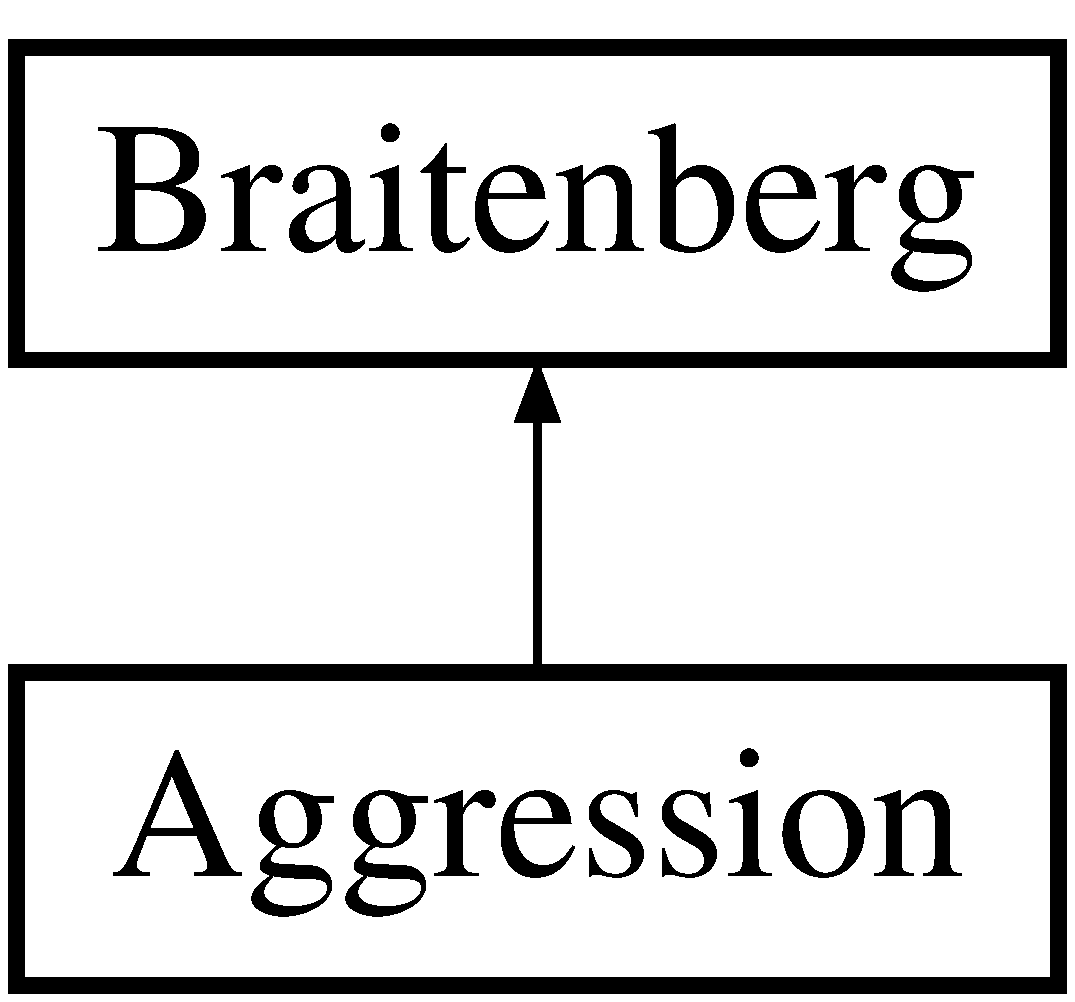
\includegraphics[height=2.000000cm]{class_aggression}
\end{center}
\end{figure}
\subsection*{Public Member Functions}
\begin{DoxyCompactItemize}
\item 
\mbox{\Hypertarget{class_aggression_adcab01129d24dc528ecbe51f474facc6}\label{class_aggression_adcab01129d24dc528ecbe51f474facc6}} 
\mbox{\hyperlink{class_aggression_adcab01129d24dc528ecbe51f474facc6}{Aggression}} ()
\begin{DoxyCompactList}\small\item\em Empty default constructor. \end{DoxyCompactList}\item 
\mbox{\Hypertarget{class_aggression_ac9851ee6b8615085c2d7235dce97e4b6}\label{class_aggression_ac9851ee6b8615085c2d7235dce97e4b6}} 
virtual \mbox{\hyperlink{class_aggression_ac9851ee6b8615085c2d7235dce97e4b6}{$\sim$\+Aggression}} ()=default
\begin{DoxyCompactList}\small\item\em Default destructors. \end{DoxyCompactList}\item 
\mbox{\hyperlink{struct_wheel_velocity}{Wheel\+Velocity}} \mbox{\hyperlink{class_aggression_ac1d60760573a45bfa025c08f33c5fe96}{Calc\+Wheel\+Velocity}} (double left\+\_\+reading, double right\+\_\+reading) override
\begin{DoxyCompactList}\small\item\em Determine the speed of both wheels based upon the robots proximity to the food. \end{DoxyCompactList}\end{DoxyCompactItemize}


\subsection{Detailed Description}
The class for the robot aggression behavior. 

This class inherits from \mbox{\hyperlink{class_braitenberg}{Braitenberg}} and overrides its Calc\+Wheel\+Velocity method. This method makes the robot go quickly towards food 

\subsection{Member Function Documentation}
\mbox{\Hypertarget{class_aggression_ac1d60760573a45bfa025c08f33c5fe96}\label{class_aggression_ac1d60760573a45bfa025c08f33c5fe96}} 
\index{Aggression@{Aggression}!Calc\+Wheel\+Velocity@{Calc\+Wheel\+Velocity}}
\index{Calc\+Wheel\+Velocity@{Calc\+Wheel\+Velocity}!Aggression@{Aggression}}
\subsubsection{\texorpdfstring{Calc\+Wheel\+Velocity()}{CalcWheelVelocity()}}
{\footnotesize\ttfamily \mbox{\hyperlink{struct_wheel_velocity}{Wheel\+Velocity}} Aggression\+::\+Calc\+Wheel\+Velocity (\begin{DoxyParamCaption}\item[{double}]{left\+\_\+reading,  }\item[{double}]{right\+\_\+reading }\end{DoxyParamCaption})\hspace{0.3cm}{\ttfamily [override]}}



Determine the speed of both wheels based upon the robots proximity to the food. 


\begin{DoxyParams}[1]{Parameters}
\mbox{\tt in}  & {\em left\+\_\+reading} & -\/ reading for food sensor on the left \\
\hline
\mbox{\tt in}  & {\em right\+\_\+reading} & -\/ reading for food sensor on the right \\
\hline
\mbox{\tt out}  & {\em The} & proper wheel velocities \\
\hline
\end{DoxyParams}


The documentation for this class was generated from the following files\+:\begin{DoxyCompactItemize}
\item 
src/\mbox{\hyperlink{aggression_8h}{aggression.\+h}}\item 
src/\mbox{\hyperlink{aggression_8cc}{aggression.\+cc}}\end{DoxyCompactItemize}

\hypertarget{class_arena}{}\section{Arena Class Reference}
\label{class_arena}\index{Arena@{Arena}}


The main class for the simulation of a 2D world with many entities running around.  




{\ttfamily \#include $<$arena.\+h$>$}

\subsection*{Public Member Functions}
\begin{DoxyCompactItemize}
\item 
\mbox{\hyperlink{class_arena_ac442d519facc5feebfd7612a53817e9a}{Arena}} (const struct \mbox{\hyperlink{structarena__params}{arena\+\_\+params}} $\ast$const params)
\begin{DoxyCompactList}\small\item\em \mbox{\hyperlink{class_arena}{Arena}}\textquotesingle{}s constructor. \end{DoxyCompactList}\item 
\mbox{\Hypertarget{class_arena_ae21b399e9e3f6b8ac4ecc44d7d1667fc}\label{class_arena_ae21b399e9e3f6b8ac4ecc44d7d1667fc}} 
\mbox{\hyperlink{class_arena_ae21b399e9e3f6b8ac4ecc44d7d1667fc}{$\sim$\+Arena}} ()
\begin{DoxyCompactList}\small\item\em \mbox{\hyperlink{class_arena}{Arena}}\textquotesingle{}s destructor. {\ttfamily delete} all entities created. \end{DoxyCompactList}\item 
void \mbox{\hyperlink{class_arena_ad92d8b2e1593b652445e31d173977fc6}{Advance\+Time}} (double dt)
\begin{DoxyCompactList}\small\item\em Advance the simulation by the specified \# of steps. \end{DoxyCompactList}\item 
\mbox{\Hypertarget{class_arena_a2b58dc065e042f825fcb97f8d8653b44}\label{class_arena_a2b58dc065e042f825fcb97f8d8653b44}} 
void \mbox{\hyperlink{class_arena_a2b58dc065e042f825fcb97f8d8653b44}{Add\+Robot}} (int quantity)
\begin{DoxyCompactList}\small\item\em Adds a \char`\"{}quantity\char`\"{} number of robots to the arena. \end{DoxyCompactList}\item 
\mbox{\Hypertarget{class_arena_a096bfda0e247cf61c3adeddcf85e525c}\label{class_arena_a096bfda0e247cf61c3adeddcf85e525c}} 
void \mbox{\hyperlink{class_arena_a096bfda0e247cf61c3adeddcf85e525c}{Add\+Fear\+Robot}} (int quantity)
\begin{DoxyCompactList}\small\item\em Adds a \char`\"{}quantity\char`\"{} number of fear robots to the arena. \end{DoxyCompactList}\item 
\mbox{\Hypertarget{class_arena_a437042b7bec3bf0d0142b576f27c0d80}\label{class_arena_a437042b7bec3bf0d0142b576f27c0d80}} 
void \mbox{\hyperlink{class_arena_a437042b7bec3bf0d0142b576f27c0d80}{Add\+Explore\+Robot}} (int quantity)
\begin{DoxyCompactList}\small\item\em Adds a \char`\"{}quantity\char`\"{} number of explore robots to the arena. \end{DoxyCompactList}\item 
\mbox{\Hypertarget{class_arena_ab369fb4240dd226c2aa1226f261d76d8}\label{class_arena_ab369fb4240dd226c2aa1226f261d76d8}} 
void \mbox{\hyperlink{class_arena_ab369fb4240dd226c2aa1226f261d76d8}{Remove\+Fear\+Robot}} (int quantity)
\begin{DoxyCompactList}\small\item\em Removes a \char`\"{}quantity\char`\"{} number of robots from the arena. \end{DoxyCompactList}\item 
\mbox{\Hypertarget{class_arena_acbda840f62b571747d2cdc2e981dbcf8}\label{class_arena_acbda840f62b571747d2cdc2e981dbcf8}} 
void \mbox{\hyperlink{class_arena_acbda840f62b571747d2cdc2e981dbcf8}{Remove\+Explore\+Robot}} (int quantity)
\begin{DoxyCompactList}\small\item\em Removes a \char`\"{}quantity\char`\"{} number of robots from the arena. \end{DoxyCompactList}\item 
\mbox{\Hypertarget{class_arena_aab318a21d3edcf5e3a5f2b3d569f9df4}\label{class_arena_aab318a21d3edcf5e3a5f2b3d569f9df4}} 
void \mbox{\hyperlink{class_arena_aab318a21d3edcf5e3a5f2b3d569f9df4}{Remove\+Light}} (int quantity)
\begin{DoxyCompactList}\small\item\em Removes a \char`\"{}quantity\char`\"{} number of lights from the arena. \end{DoxyCompactList}\item 
\mbox{\Hypertarget{class_arena_afe8183aefcc378cff0d4eda15dd49cb9}\label{class_arena_afe8183aefcc378cff0d4eda15dd49cb9}} 
void \mbox{\hyperlink{class_arena_afe8183aefcc378cff0d4eda15dd49cb9}{Remove\+Food}} (int quantity)
\begin{DoxyCompactList}\small\item\em Removes a \char`\"{}quantity\char`\"{} number of lights from the arena. \end{DoxyCompactList}\item 
\mbox{\Hypertarget{class_arena_a6c32af2d77a9afde2a41aa7359a62763}\label{class_arena_a6c32af2d77a9afde2a41aa7359a62763}} 
void \mbox{\hyperlink{class_arena_a6c32af2d77a9afde2a41aa7359a62763}{Add\+Light}} (int quantity)
\begin{DoxyCompactList}\small\item\em Adds a \char`\"{}quantity\char`\"{} number of lights to the arena. \end{DoxyCompactList}\item 
\mbox{\Hypertarget{class_arena_a663b46b86ee69523e993ec38d079c482}\label{class_arena_a663b46b86ee69523e993ec38d079c482}} 
void \mbox{\hyperlink{class_arena_a663b46b86ee69523e993ec38d079c482}{Add\+Food}} (int quantity)
\begin{DoxyCompactList}\small\item\em Adds a \char`\"{}quantity\char`\"{} number of food to the arena. \end{DoxyCompactList}\item 
void \mbox{\hyperlink{class_arena_a16fac8e4b2399fcf0db01a9722069c33}{Accept\+Command}} (Communication com)
\begin{DoxyCompactList}\small\item\em Accepts a screen command and performs a task accordingly. \end{DoxyCompactList}\item 
\mbox{\Hypertarget{class_arena_a95e295d03a14385f4402a8e839fbae9b}\label{class_arena_a95e295d03a14385f4402a8e839fbae9b}} 
void \mbox{\hyperlink{class_arena_a95e295d03a14385f4402a8e839fbae9b}{Reset}} ()
\begin{DoxyCompactList}\small\item\em Reset all entities in \mbox{\hyperlink{class_arena}{Arena}}. \end{DoxyCompactList}\item 
\mbox{\Hypertarget{class_arena_aa977a50aa4a5570a2a553705f1909e9b}\label{class_arena_aa977a50aa4a5570a2a553705f1909e9b}} 
\mbox{\hyperlink{class_arena}{Arena}} \& \mbox{\hyperlink{class_arena_aa977a50aa4a5570a2a553705f1909e9b}{operator=}} (const \mbox{\hyperlink{class_arena}{Arena}} \&other)=delete
\begin{DoxyCompactList}\small\item\em Under certain circumstance, the compiler requires that the assignment operator is not defined. This {\ttfamily deletes} the default assignment operator. \end{DoxyCompactList}\item 
\mbox{\Hypertarget{class_arena_afce6e35e1470823539dc9194bef77499}\label{class_arena_afce6e35e1470823539dc9194bef77499}} 
\mbox{\hyperlink{class_arena_afce6e35e1470823539dc9194bef77499}{Arena}} (const \mbox{\hyperlink{class_arena}{Arena}} \&other)=delete
\begin{DoxyCompactList}\small\item\em Under certain circumstance, the compiler requires that the copy constructor is not defined. This {\ttfamily deletes} the default copy constructor. \end{DoxyCompactList}\item 
bool \mbox{\hyperlink{class_arena_ab4479b0268867602d0c4b510d5f99aff}{Is\+Colliding}} (\mbox{\hyperlink{class_arena_mobile_entity}{Arena\+Mobile\+Entity}} $\ast$const mobile\+\_\+e, \mbox{\hyperlink{class_arena_entity}{Arena\+Entity}} $\ast$const other\+\_\+e)
\begin{DoxyCompactList}\small\item\em Determine if two entities have collided in the \mbox{\hyperlink{class_arena}{Arena}}. Collision is defined as the distance between two entities being less than the sum of their radii. \end{DoxyCompactList}\item 
\mbox{\Hypertarget{class_arena_a2506fab770b6070d8f061bcab4c65138}\label{class_arena_a2506fab770b6070d8f061bcab4c65138}} 
void \mbox{\hyperlink{class_arena_a2506fab770b6070d8f061bcab4c65138}{Adjust\+Entity\+Overlap}} (\mbox{\hyperlink{class_arena_mobile_entity}{Arena\+Mobile\+Entity}} $\ast$const mobile\+\_\+e, \mbox{\hyperlink{class_arena_entity}{Arena\+Entity}} $\ast$const other\+\_\+e)
\begin{DoxyCompactList}\small\item\em Move the mobile entity to the edge of the other without overlap. Without this, entities tend to get stuck inside one another. \end{DoxyCompactList}\item 
Entity\+Type \mbox{\hyperlink{class_arena_a7b72cf7688ee6ab1395bf438663bc1da}{Get\+Collision\+Wall}} (\mbox{\hyperlink{class_arena_mobile_entity}{Arena\+Mobile\+Entity}} $\ast$const ent)
\begin{DoxyCompactList}\small\item\em Determine if a particular entity has gone out of the boundaries of the simulation (i.\+e. has collided with any one of the walls). \end{DoxyCompactList}\item 
\mbox{\Hypertarget{class_arena_a51c1e99dfd9a618c6041fd22d0a11959}\label{class_arena_a51c1e99dfd9a618c6041fd22d0a11959}} 
void \mbox{\hyperlink{class_arena_a51c1e99dfd9a618c6041fd22d0a11959}{Adjust\+Wall\+Overlap}} (\mbox{\hyperlink{class_arena_mobile_entity}{Arena\+Mobile\+Entity}} $\ast$const ent, Entity\+Type wall)
\begin{DoxyCompactList}\small\item\em Move the entity to the edge of the wall without overlap. Without this, entities tend to get stuck in walls. \end{DoxyCompactList}\item 
void \mbox{\hyperlink{class_arena_a682ec81cb30e36e5bb801b3388bcb494}{Update\+Entities\+Timestep}} ()
\begin{DoxyCompactList}\small\item\em Update all entities for a single timestep. \end{DoxyCompactList}\item 
\mbox{\Hypertarget{class_arena_a952408e8197790a034b75a4e275bcbc2}\label{class_arena_a952408e8197790a034b75a4e275bcbc2}} 
std\+::vector$<$ class \mbox{\hyperlink{class_arena_entity}{Arena\+Entity}} $\ast$ $>$ \mbox{\hyperlink{class_arena_a952408e8197790a034b75a4e275bcbc2}{get\+\_\+entities}} () const
\begin{DoxyCompactList}\small\item\em Returns all of the entities. \end{DoxyCompactList}\item 
\mbox{\Hypertarget{class_arena_a40a7597d65a8ed5020aba4025b35617b}\label{class_arena_a40a7597d65a8ed5020aba4025b35617b}} 
std\+::vector$<$ class \mbox{\hyperlink{class_arena_mobile_entity}{Arena\+Mobile\+Entity}} $\ast$ $>$ \mbox{\hyperlink{class_arena_a40a7597d65a8ed5020aba4025b35617b}{get\+\_\+mobile\+\_\+entities}} () const
\begin{DoxyCompactList}\small\item\em Returns all of the mobile entities. \end{DoxyCompactList}\item 
\mbox{\Hypertarget{class_arena_a5e3be20f2c67338a5a684b85a66f6b96}\label{class_arena_a5e3be20f2c67338a5a684b85a66f6b96}} 
double \mbox{\hyperlink{class_arena_a5e3be20f2c67338a5a684b85a66f6b96}{get\+\_\+x\+\_\+dim}} ()
\begin{DoxyCompactList}\small\item\em Returns the x dimension of the graphics window. \end{DoxyCompactList}\item 
\mbox{\Hypertarget{class_arena_a35737d65ff32f2bd5871f0bdfbc10a85}\label{class_arena_a35737d65ff32f2bd5871f0bdfbc10a85}} 
double \mbox{\hyperlink{class_arena_a35737d65ff32f2bd5871f0bdfbc10a85}{get\+\_\+y\+\_\+dim}} ()
\begin{DoxyCompactList}\small\item\em Returns the y dimension of the graphics window. \end{DoxyCompactList}\item 
\mbox{\Hypertarget{class_arena_a4d599cccea003b9c60ddb39535c058f4}\label{class_arena_a4d599cccea003b9c60ddb39535c058f4}} 
int \mbox{\hyperlink{class_arena_a4d599cccea003b9c60ddb39535c058f4}{get\+\_\+game\+\_\+status}} () const
\begin{DoxyCompactList}\small\item\em Returns the game status. \end{DoxyCompactList}\item 
\mbox{\Hypertarget{class_arena_ac8e8b3438db02aa5395f7fcb537ed952}\label{class_arena_ac8e8b3438db02aa5395f7fcb537ed952}} 
void \mbox{\hyperlink{class_arena_ac8e8b3438db02aa5395f7fcb537ed952}{set\+\_\+game\+\_\+status}} (int status)
\begin{DoxyCompactList}\small\item\em Sets the game status to playing or paused. \end{DoxyCompactList}\item 
\mbox{\Hypertarget{class_arena_a92e4a5857a642909af5e76e8b8129f03}\label{class_arena_a92e4a5857a642909af5e76e8b8129f03}} 
void \mbox{\hyperlink{class_arena_a92e4a5857a642909af5e76e8b8129f03}{set\+\_\+paused}} (bool paused)
\begin{DoxyCompactList}\small\item\em Sets whether the game is paused or not. \end{DoxyCompactList}\item 
\mbox{\Hypertarget{class_arena_a3b39ca9d3b5974b93d49317e43485962}\label{class_arena_a3b39ca9d3b5974b93d49317e43485962}} 
bool \mbox{\hyperlink{class_arena_a3b39ca9d3b5974b93d49317e43485962}{get\+\_\+paused}} (void)
\begin{DoxyCompactList}\small\item\em Returns if the game is paused or not. \end{DoxyCompactList}\item 
\mbox{\Hypertarget{class_arena_a684050e2bd1c7a6ecb57c38575fec995}\label{class_arena_a684050e2bd1c7a6ecb57c38575fec995}} 
\mbox{\hyperlink{class_entity_factory}{Entity\+Factory}} $\ast$ {\bfseries get\+\_\+factory} ()
\item 
\mbox{\Hypertarget{class_arena_abc2f835afc51723b80fb53310e6c4864}\label{class_arena_abc2f835afc51723b80fb53310e6c4864}} 
int {\bfseries get\+\_\+num\+\_\+fear\+\_\+robots} ()
\item 
\mbox{\Hypertarget{class_arena_a8fdca5473b8a8795a241f2a7ade172c2}\label{class_arena_a8fdca5473b8a8795a241f2a7ade172c2}} 
int {\bfseries get\+\_\+num\+\_\+explore\+\_\+robots} ()
\item 
\mbox{\Hypertarget{class_arena_a0b6b09dbeb919c2300dc034a39cbe57f}\label{class_arena_a0b6b09dbeb919c2300dc034a39cbe57f}} 
int {\bfseries get\+\_\+num\+\_\+robots} ()
\end{DoxyCompactItemize}


\subsection{Detailed Description}
The main class for the simulation of a 2D world with many entities running around. 

While \mbox{\hyperlink{class_graphics_arena_viewer}{Graphics\+Arena\+Viewer}} handles the graphics, \mbox{\hyperlink{class_arena}{Arena}} handles all the data and all the entities (it is the model of M\+VC). It manages the interaction among the entities in the \mbox{\hyperlink{class_arena}{Arena}}. 

\subsection{Constructor \& Destructor Documentation}
\mbox{\Hypertarget{class_arena_ac442d519facc5feebfd7612a53817e9a}\label{class_arena_ac442d519facc5feebfd7612a53817e9a}} 
\index{Arena@{Arena}!Arena@{Arena}}
\index{Arena@{Arena}!Arena@{Arena}}
\subsubsection{\texorpdfstring{Arena()}{Arena()}}
{\footnotesize\ttfamily Arena\+::\+Arena (\begin{DoxyParamCaption}\item[{const struct \mbox{\hyperlink{structarena__params}{arena\+\_\+params}} $\ast$const}]{params }\end{DoxyParamCaption})\hspace{0.3cm}{\ttfamily [explicit]}}



\mbox{\hyperlink{class_arena}{Arena}}\textquotesingle{}s constructor. 


\begin{DoxyParams}{Parameters}
{\em params} & A \mbox{\hyperlink{structarena__params}{arena\+\_\+params}} passed down from \mbox{\hyperlink{main_8cc}{main.\+cc}} for the initialization of \mbox{\hyperlink{class_arena}{Arena}} and the entities therein.\\
\hline
\end{DoxyParams}
Initialize all private variables and entities. 

\subsection{Member Function Documentation}
\mbox{\Hypertarget{class_arena_a16fac8e4b2399fcf0db01a9722069c33}\label{class_arena_a16fac8e4b2399fcf0db01a9722069c33}} 
\index{Arena@{Arena}!Accept\+Command@{Accept\+Command}}
\index{Accept\+Command@{Accept\+Command}!Arena@{Arena}}
\subsubsection{\texorpdfstring{Accept\+Command()}{AcceptCommand()}}
{\footnotesize\ttfamily void Arena\+::\+Accept\+Command (\begin{DoxyParamCaption}\item[{Communication}]{com }\end{DoxyParamCaption})}



Accepts a screen command and performs a task accordingly. 

Accepting commands for playing and pausing the game as well as setting a new game. \mbox{\Hypertarget{class_arena_ad92d8b2e1593b652445e31d173977fc6}\label{class_arena_ad92d8b2e1593b652445e31d173977fc6}} 
\index{Arena@{Arena}!Advance\+Time@{Advance\+Time}}
\index{Advance\+Time@{Advance\+Time}!Arena@{Arena}}
\subsubsection{\texorpdfstring{Advance\+Time()}{AdvanceTime()}}
{\footnotesize\ttfamily void Arena\+::\+Advance\+Time (\begin{DoxyParamCaption}\item[{double}]{dt }\end{DoxyParamCaption})}



Advance the simulation by the specified \# of steps. 


\begin{DoxyParams}[1]{Parameters}
\mbox{\tt in}  & {\em dt} & The \# of steps to increment by. This is practically unused because the arena state is advanced incrementally at a fixed rate.\\
\hline
\end{DoxyParams}
If {\ttfamily dt == 0}, {\ttfamily return} immediately. Otherwise calls \mbox{\hyperlink{class_arena_a682ec81cb30e36e5bb801b3388bcb494}{Arena\+::\+Update\+Entities\+Timestep()}} once. \mbox{\Hypertarget{class_arena_a7b72cf7688ee6ab1395bf438663bc1da}\label{class_arena_a7b72cf7688ee6ab1395bf438663bc1da}} 
\index{Arena@{Arena}!Get\+Collision\+Wall@{Get\+Collision\+Wall}}
\index{Get\+Collision\+Wall@{Get\+Collision\+Wall}!Arena@{Arena}}
\subsubsection{\texorpdfstring{Get\+Collision\+Wall()}{GetCollisionWall()}}
{\footnotesize\ttfamily Entity\+Type Arena\+::\+Get\+Collision\+Wall (\begin{DoxyParamCaption}\item[{\mbox{\hyperlink{class_arena_mobile_entity}{Arena\+Mobile\+Entity}} $\ast$const}]{ent }\end{DoxyParamCaption})}



Determine if a particular entity has gone out of the boundaries of the simulation (i.\+e. has collided with any one of the walls). 


\begin{DoxyParams}[1]{Parameters}
 & {\em ent} & The entity to check. \\
\hline
\mbox{\tt out}  & {\em An} & entity type signifying wall (e.\+g. k\+Right\+Wall). k\+Undefined if no collision.\\
\hline
\end{DoxyParams}
The checked entity\textquotesingle{}s position will be updated to a \char`\"{}back-\/off position\char`\"{} so that it won\textquotesingle{}t get stuck into a wall. The calculation of the \char`\"{}back-\/off
position\char`\"{} is technically not accurate, but good enough for our purpose. \mbox{\Hypertarget{class_arena_ab4479b0268867602d0c4b510d5f99aff}\label{class_arena_ab4479b0268867602d0c4b510d5f99aff}} 
\index{Arena@{Arena}!Is\+Colliding@{Is\+Colliding}}
\index{Is\+Colliding@{Is\+Colliding}!Arena@{Arena}}
\subsubsection{\texorpdfstring{Is\+Colliding()}{IsColliding()}}
{\footnotesize\ttfamily bool Arena\+::\+Is\+Colliding (\begin{DoxyParamCaption}\item[{\mbox{\hyperlink{class_arena_mobile_entity}{Arena\+Mobile\+Entity}} $\ast$const}]{mobile\+\_\+e,  }\item[{\mbox{\hyperlink{class_arena_entity}{Arena\+Entity}} $\ast$const}]{other\+\_\+e }\end{DoxyParamCaption})}



Determine if two entities have collided in the \mbox{\hyperlink{class_arena}{Arena}}. Collision is defined as the distance between two entities being less than the sum of their radii. 


\begin{DoxyParams}[1]{Parameters}
 & {\em mobile\+\_\+e} & This entity is definitely moving. \\
\hline
 & {\em other\+\_\+e} & This entity might be mobile or immobile. \\
\hline
\mbox{\tt out}  & {\em True} & if entities overlapping. \\
\hline
\end{DoxyParams}
\mbox{\Hypertarget{class_arena_a682ec81cb30e36e5bb801b3388bcb494}\label{class_arena_a682ec81cb30e36e5bb801b3388bcb494}} 
\index{Arena@{Arena}!Update\+Entities\+Timestep@{Update\+Entities\+Timestep}}
\index{Update\+Entities\+Timestep@{Update\+Entities\+Timestep}!Arena@{Arena}}
\subsubsection{\texorpdfstring{Update\+Entities\+Timestep()}{UpdateEntitiesTimestep()}}
{\footnotesize\ttfamily void Arena\+::\+Update\+Entities\+Timestep (\begin{DoxyParamCaption}{ }\end{DoxyParamCaption})}



Update all entities for a single timestep. 

First calls each entity\textquotesingle{}s Timestep\+Update method to update their speed, heading angle, and position. Then check for collisions between entities or between an entity and a wall. 

The documentation for this class was generated from the following files\+:\begin{DoxyCompactItemize}
\item 
src/\mbox{\hyperlink{arena_8h}{arena.\+h}}\item 
src/\mbox{\hyperlink{arena_8cc}{arena.\+cc}}\end{DoxyCompactItemize}

\hypertarget{structarena__params}{}\section{arena\+\_\+params Struct Reference}
\label{structarena__params}\index{arena\+\_\+params@{arena\+\_\+params}}


Struct holding parameters for initializing the \mbox{\hyperlink{class_arena}{Arena}}.  




{\ttfamily \#include $<$arena\+\_\+params.\+h$>$}

\subsection*{Public Attributes}
\begin{DoxyCompactItemize}
\item 
\mbox{\Hypertarget{structarena__params_a98012558dd0075a9f0df9f38140c5bbd}\label{structarena__params_a98012558dd0075a9f0df9f38140c5bbd}} 
size\+\_\+t {\bfseries n\+\_\+lights} \{N\+\_\+\+L\+I\+G\+H\+TS\}
\item 
\mbox{\Hypertarget{structarena__params_a4160066249e38b463e638d0f8478a5c1}\label{structarena__params_a4160066249e38b463e638d0f8478a5c1}} 
size\+\_\+t {\bfseries n\+\_\+foods} \{N\+\_\+\+F\+O\+O\+DS\}
\item 
\mbox{\Hypertarget{structarena__params_a6ae235113b4a6870d502c913c65ad9a2}\label{structarena__params_a6ae235113b4a6870d502c913c65ad9a2}} 
size\+\_\+t {\bfseries n\+\_\+robots} \{N\+\_\+\+R\+O\+B\+O\+TS\}
\item 
\mbox{\Hypertarget{structarena__params_afa86b434ed8ea5a4fe9ae14ae1438e8f}\label{structarena__params_afa86b434ed8ea5a4fe9ae14ae1438e8f}} 
uint {\bfseries x\+\_\+dim} \{A\+R\+E\+N\+A\+\_\+\+X\+\_\+\+D\+IM\}
\item 
\mbox{\Hypertarget{structarena__params_ab5d50b9affa9c753c15e1d6f088824af}\label{structarena__params_ab5d50b9affa9c753c15e1d6f088824af}} 
uint {\bfseries y\+\_\+dim} \{A\+R\+E\+N\+A\+\_\+\+Y\+\_\+\+D\+IM\}
\end{DoxyCompactItemize}


\subsection{Detailed Description}
Struct holding parameters for initializing the \mbox{\hyperlink{class_arena}{Arena}}. 

These parameters include the parameters for \mbox{\hyperlink{class_arena}{Arena}}\textquotesingle{}s geometry as well as the parameters for initializing A\+LL entities within the \mbox{\hyperlink{class_arena}{Arena}}. 

The documentation for this struct was generated from the following file\+:\begin{DoxyCompactItemize}
\item 
src/\mbox{\hyperlink{arena__params_8h}{arena\+\_\+params.\+h}}\end{DoxyCompactItemize}

\hypertarget{class_arena_entity}{}\section{Arena\+Entity Class Reference}
\label{class_arena_entity}\index{Arena\+Entity@{Arena\+Entity}}


A food class from which all \mbox{\hyperlink{class_arena}{Arena}} entities inherit.  




{\ttfamily \#include $<$arena\+\_\+entity.\+h$>$}

Inheritance diagram for Arena\+Entity\+:\begin{figure}[H]
\begin{center}
\leavevmode
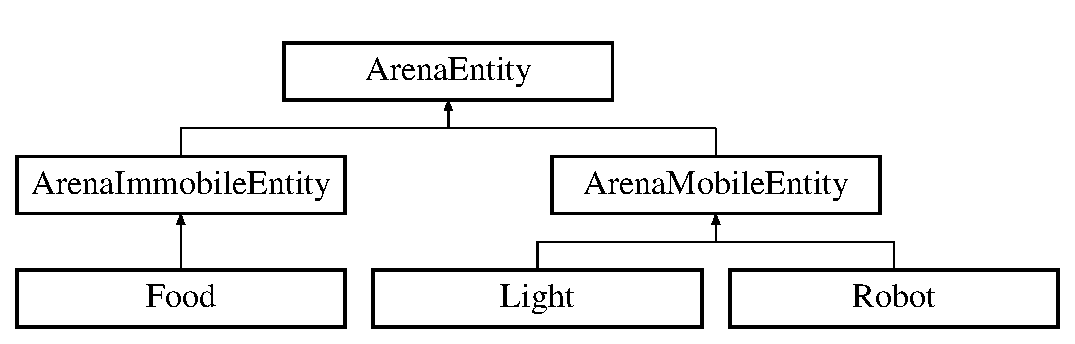
\includegraphics[height=3.000000cm]{class_arena_entity}
\end{center}
\end{figure}
\subsection*{Public Member Functions}
\begin{DoxyCompactItemize}
\item 
\mbox{\Hypertarget{class_arena_entity_a96df749814e89344a6149e4da89b4e44}\label{class_arena_entity_a96df749814e89344a6149e4da89b4e44}} 
\mbox{\hyperlink{class_arena_entity_a96df749814e89344a6149e4da89b4e44}{Arena\+Entity}} ()
\begin{DoxyCompactList}\small\item\em \mbox{\hyperlink{class_arena_entity}{Arena\+Entity}} constructor initialized with default values from \mbox{\hyperlink{params_8h}{params.\+h}}. \end{DoxyCompactList}\item 
\mbox{\Hypertarget{class_arena_entity_aa7af53e5d8830d144ccf2ad07d9140da}\label{class_arena_entity_aa7af53e5d8830d144ccf2ad07d9140da}} 
virtual \mbox{\hyperlink{class_arena_entity_aa7af53e5d8830d144ccf2ad07d9140da}{$\sim$\+Arena\+Entity}} ()=default
\begin{DoxyCompactList}\small\item\em Default destructor -- as defined by compiler. \end{DoxyCompactList}\item 
virtual void \mbox{\hyperlink{class_arena_entity_a203613c40a5cecf47606b2a59adcc3bd}{Timestep\+Update}} (\mbox{\hyperlink{common_8h_a2e3484535ee610c8e19e9859563abe48}{\+\_\+\+\_\+unused}} unsigned int dt)
\begin{DoxyCompactList}\small\item\em Perform whatever updates needed for a particular entity after 1 timestep (updating position, changing color, etc.). \end{DoxyCompactList}\item 
\mbox{\Hypertarget{class_arena_entity_abaebe6c02659e22c08579d49829c5676}\label{class_arena_entity_abaebe6c02659e22c08579d49829c5676}} 
virtual void \mbox{\hyperlink{class_arena_entity_abaebe6c02659e22c08579d49829c5676}{Reset}} ()
\begin{DoxyCompactList}\small\item\em Reset entity to a newly constructed state. \end{DoxyCompactList}\item 
virtual std\+::string \mbox{\hyperlink{class_arena_entity_ad43152003033cf01ad86eeff1990b69a}{get\+\_\+name}} () const =0
\begin{DoxyCompactList}\small\item\em Get the name of the entity for visualization and for debugging. \end{DoxyCompactList}\item 
\mbox{\Hypertarget{class_arena_entity_a9a0efa995da3ed55e92f54357fd2bdae}\label{class_arena_entity_a9a0efa995da3ed55e92f54357fd2bdae}} 
const \mbox{\hyperlink{struct_pose}{Pose}} \& \mbox{\hyperlink{class_arena_entity_a9a0efa995da3ed55e92f54357fd2bdae}{get\+\_\+pose}} () const
\begin{DoxyCompactList}\small\item\em Returns the postion of the entity. \end{DoxyCompactList}\item 
\mbox{\Hypertarget{class_arena_entity_a6eb76e5f1b5949314c12cc512d6930ae}\label{class_arena_entity_a6eb76e5f1b5949314c12cc512d6930ae}} 
void \mbox{\hyperlink{class_arena_entity_a6eb76e5f1b5949314c12cc512d6930ae}{set\+\_\+pose}} (const \mbox{\hyperlink{struct_pose}{Pose}} \&pose)
\begin{DoxyCompactList}\small\item\em Sets the position of the entity. \end{DoxyCompactList}\item 
\mbox{\Hypertarget{class_arena_entity_a3136704edf07c24639319abf5c28dac0}\label{class_arena_entity_a3136704edf07c24639319abf5c28dac0}} 
void \mbox{\hyperlink{class_arena_entity_a3136704edf07c24639319abf5c28dac0}{set\+\_\+position}} (const double inx, const double iny)
\begin{DoxyCompactList}\small\item\em Setter method for position within entity pose variable. \end{DoxyCompactList}\item 
\mbox{\Hypertarget{class_arena_entity_ac1cc3c6997bc7a9573128fc5ded9eb72}\label{class_arena_entity_ac1cc3c6997bc7a9573128fc5ded9eb72}} 
void \mbox{\hyperlink{class_arena_entity_ac1cc3c6997bc7a9573128fc5ded9eb72}{set\+\_\+heading}} (const double t)
\begin{DoxyCompactList}\small\item\em Setter method for heading within entity pose variable. \end{DoxyCompactList}\item 
void \mbox{\hyperlink{class_arena_entity_a4c4bd7f5ffb778979303c33cb3bc9986}{Relative\+Change\+Heading}} (const double delta)
\begin{DoxyCompactList}\small\item\em Setter for heading within pose, but change is relative to current value. \end{DoxyCompactList}\item 
\mbox{\Hypertarget{class_arena_entity_a5790a5d45229aa76223a8183ac916323}\label{class_arena_entity_a5790a5d45229aa76223a8183ac916323}} 
const \mbox{\hyperlink{struct_rgb_color}{Rgb\+Color}} \& \mbox{\hyperlink{class_arena_entity_a5790a5d45229aa76223a8183ac916323}{get\+\_\+color}} () const
\begin{DoxyCompactList}\small\item\em Returns the color of the entity. \end{DoxyCompactList}\item 
\mbox{\Hypertarget{class_arena_entity_a1ac33beda7462ac5c7f4f71a70d3fb10}\label{class_arena_entity_a1ac33beda7462ac5c7f4f71a70d3fb10}} 
void \mbox{\hyperlink{class_arena_entity_a1ac33beda7462ac5c7f4f71a70d3fb10}{set\+\_\+color}} (const \mbox{\hyperlink{struct_rgb_color}{Rgb\+Color}} \&color)
\begin{DoxyCompactList}\small\item\em Sets the color of the entity. \end{DoxyCompactList}\item 
\mbox{\Hypertarget{class_arena_entity_a42d86d2d952b7f2a861d8a6cb46e661e}\label{class_arena_entity_a42d86d2d952b7f2a861d8a6cb46e661e}} 
double \mbox{\hyperlink{class_arena_entity_a42d86d2d952b7f2a861d8a6cb46e661e}{get\+\_\+radius}} () const
\begin{DoxyCompactList}\small\item\em Returns the radius of the entity. \end{DoxyCompactList}\item 
\mbox{\Hypertarget{class_arena_entity_a2b0c2512fe53d143442da5e357f71505}\label{class_arena_entity_a2b0c2512fe53d143442da5e357f71505}} 
void \mbox{\hyperlink{class_arena_entity_a2b0c2512fe53d143442da5e357f71505}{set\+\_\+radius}} (double radius)
\begin{DoxyCompactList}\small\item\em Sets the radius of the entity. \end{DoxyCompactList}\item 
\mbox{\Hypertarget{class_arena_entity_a19e75df5ce971f48e9a522a343a39fb3}\label{class_arena_entity_a19e75df5ce971f48e9a522a343a39fb3}} 
Entity\+Type \mbox{\hyperlink{class_arena_entity_a19e75df5ce971f48e9a522a343a39fb3}{get\+\_\+type}} () const
\begin{DoxyCompactList}\small\item\em Returns the type of the entity. \end{DoxyCompactList}\item 
\mbox{\Hypertarget{class_arena_entity_aa65c584906d4c22f61488fab98c3392c}\label{class_arena_entity_aa65c584906d4c22f61488fab98c3392c}} 
void \mbox{\hyperlink{class_arena_entity_aa65c584906d4c22f61488fab98c3392c}{set\+\_\+type}} (Entity\+Type et)
\begin{DoxyCompactList}\small\item\em Sets the type of the entity. \end{DoxyCompactList}\item 
\mbox{\Hypertarget{class_arena_entity_ae50750dfde8118c27835ea8e9db8b7ef}\label{class_arena_entity_ae50750dfde8118c27835ea8e9db8b7ef}} 
int \mbox{\hyperlink{class_arena_entity_ae50750dfde8118c27835ea8e9db8b7ef}{get\+\_\+id}} () const
\begin{DoxyCompactList}\small\item\em Returns the id of the entity. \end{DoxyCompactList}\item 
\mbox{\Hypertarget{class_arena_entity_a67f4c0467d32eec76ee6ed033ff9ed2f}\label{class_arena_entity_a67f4c0467d32eec76ee6ed033ff9ed2f}} 
void \mbox{\hyperlink{class_arena_entity_a67f4c0467d32eec76ee6ed033ff9ed2f}{set\+\_\+id}} (int id)
\begin{DoxyCompactList}\small\item\em Sets the id of the entity. \end{DoxyCompactList}\item 
\mbox{\Hypertarget{class_arena_entity_a9cfea21220c07502abd084afde49ae65}\label{class_arena_entity_a9cfea21220c07502abd084afde49ae65}} 
bool \mbox{\hyperlink{class_arena_entity_a9cfea21220c07502abd084afde49ae65}{is\+\_\+mobile}} (void)
\begin{DoxyCompactList}\small\item\em Getter method for determining if entity can move or not. \end{DoxyCompactList}\item 
\mbox{\Hypertarget{class_arena_entity_adb5d3089fec5c28cc989e5834fcdaf6c}\label{class_arena_entity_adb5d3089fec5c28cc989e5834fcdaf6c}} 
void \mbox{\hyperlink{class_arena_entity_adb5d3089fec5c28cc989e5834fcdaf6c}{set\+\_\+mobility}} (bool value)
\begin{DoxyCompactList}\small\item\em Setter method for indicating if entity can move or not. \end{DoxyCompactList}\item 
\mbox{\Hypertarget{class_arena_entity_ad9d597b105a901a79c45cbf704c115d0}\label{class_arena_entity_ad9d597b105a901a79c45cbf704c115d0}} 
\mbox{\hyperlink{struct_pose}{Pose}} \mbox{\hyperlink{class_arena_entity_ad9d597b105a901a79c45cbf704c115d0}{Set\+Pose\+Randomly}} ()
\begin{DoxyCompactList}\small\item\em An attempt to not overlap any of the newly constructed entities. \end{DoxyCompactList}\end{DoxyCompactItemize}


\subsection{Detailed Description}
A food class from which all \mbox{\hyperlink{class_arena}{Arena}} entities inherit. 

All entities know how to\+:


\begin{DoxyEnumerate}
\item Update themselves at each timestep (i.\+e. in accordance with current velocity and position).
\item Reset themselves to a newly constructed state. So that the user can click the reset button to restart the game. Alternatively, the game will be reset if the robot has won/lost.
\end{DoxyEnumerate}

Please note that here use the upper-\/left coordinate, which means that the origin point (0.\+0,0.\+0) is at the upper left.

All arena entities are circular. 

\subsection{Member Function Documentation}
\mbox{\Hypertarget{class_arena_entity_ad43152003033cf01ad86eeff1990b69a}\label{class_arena_entity_ad43152003033cf01ad86eeff1990b69a}} 
\index{Arena\+Entity@{Arena\+Entity}!get\+\_\+name@{get\+\_\+name}}
\index{get\+\_\+name@{get\+\_\+name}!Arena\+Entity@{Arena\+Entity}}
\subsubsection{\texorpdfstring{get\+\_\+name()}{get\_name()}}
{\footnotesize\ttfamily virtual std\+::string Arena\+Entity\+::get\+\_\+name (\begin{DoxyParamCaption}{ }\end{DoxyParamCaption}) const\hspace{0.3cm}{\ttfamily [pure virtual]}}



Get the name of the entity for visualization and for debugging. 

\begin{DoxyReturn}{Returns}
Name of the entity. Each entity type hard codes its name (e.\+g. \char`\"{}\+Robot\char`\"{}). 
\end{DoxyReturn}


Implemented in \mbox{\hyperlink{class_robot_a3f77c13705b8f60480d21d8d936dc39e}{Robot}}, \mbox{\hyperlink{class_food_a5c3bcd5109750a15ebb24b8a2a3cdd07}{Food}}, and \mbox{\hyperlink{class_light_a49b2e32cf8173353ac4689fdadbb95d5}{Light}}.

\mbox{\Hypertarget{class_arena_entity_a4c4bd7f5ffb778979303c33cb3bc9986}\label{class_arena_entity_a4c4bd7f5ffb778979303c33cb3bc9986}} 
\index{Arena\+Entity@{Arena\+Entity}!Relative\+Change\+Heading@{Relative\+Change\+Heading}}
\index{Relative\+Change\+Heading@{Relative\+Change\+Heading}!Arena\+Entity@{Arena\+Entity}}
\subsubsection{\texorpdfstring{Relative\+Change\+Heading()}{RelativeChangeHeading()}}
{\footnotesize\ttfamily void Arena\+Entity\+::\+Relative\+Change\+Heading (\begin{DoxyParamCaption}\item[{const double}]{delta }\end{DoxyParamCaption})\hspace{0.3cm}{\ttfamily [inline]}}



Setter for heading within pose, but change is relative to current value. 


\begin{DoxyParams}[1]{Parameters}
\mbox{\tt in}  & {\em delta} & by which to modify current heading. Can be positive or negative. \\
\hline
\end{DoxyParams}
\mbox{\Hypertarget{class_arena_entity_a203613c40a5cecf47606b2a59adcc3bd}\label{class_arena_entity_a203613c40a5cecf47606b2a59adcc3bd}} 
\index{Arena\+Entity@{Arena\+Entity}!Timestep\+Update@{Timestep\+Update}}
\index{Timestep\+Update@{Timestep\+Update}!Arena\+Entity@{Arena\+Entity}}
\subsubsection{\texorpdfstring{Timestep\+Update()}{TimestepUpdate()}}
{\footnotesize\ttfamily virtual void Arena\+Entity\+::\+Timestep\+Update (\begin{DoxyParamCaption}\item[{\mbox{\hyperlink{common_8h_a2e3484535ee610c8e19e9859563abe48}{\+\_\+\+\_\+unused}} unsigned int}]{dt }\end{DoxyParamCaption})\hspace{0.3cm}{\ttfamily [inline]}, {\ttfamily [virtual]}}



Perform whatever updates needed for a particular entity after 1 timestep (updating position, changing color, etc.). 


\begin{DoxyParams}[1]{Parameters}
\mbox{\tt in}  & {\em dt} & is time elapsed since the last update. Unused. \\
\hline
\end{DoxyParams}


The documentation for this class was generated from the following file\+:\begin{DoxyCompactItemize}
\item 
src/\mbox{\hyperlink{arena__entity_8h}{arena\+\_\+entity.\+h}}\end{DoxyCompactItemize}

\hypertarget{class_arena_immobile_entity}{}\section{Arena\+Immobile\+Entity Class Reference}
\label{class_arena_immobile_entity}\index{Arena\+Immobile\+Entity@{Arena\+Immobile\+Entity}}


An immobile entity in the \mbox{\hyperlink{class_arena}{Arena}}.  




{\ttfamily \#include $<$arena\+\_\+immobile\+\_\+entity.\+h$>$}

Inheritance diagram for Arena\+Immobile\+Entity\+:\begin{figure}[H]
\begin{center}
\leavevmode
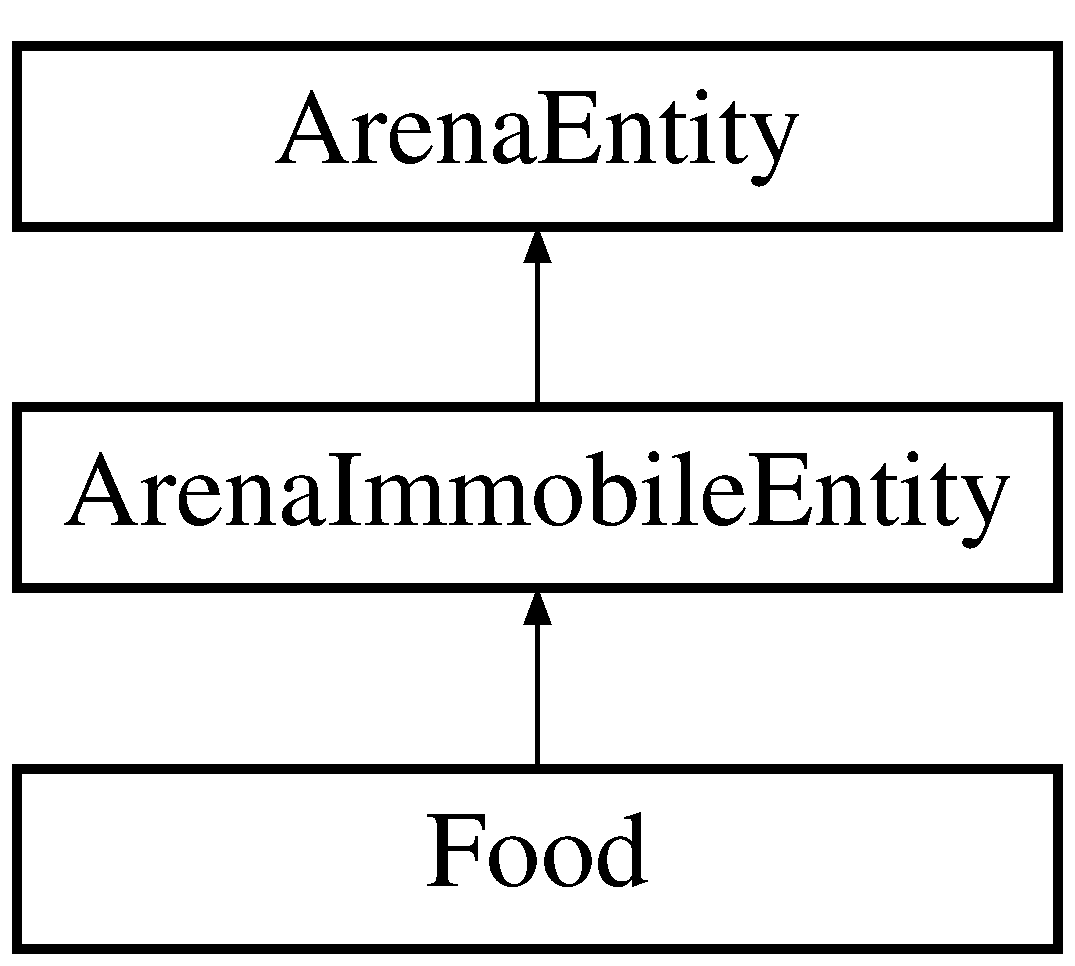
\includegraphics[height=3.000000cm]{class_arena_immobile_entity}
\end{center}
\end{figure}
\subsection*{Public Member Functions}
\begin{DoxyCompactItemize}
\item 
\mbox{\hyperlink{class_arena_immobile_entity_ac24bb0af97a140d62dd52124489032fd}{Arena\+Immobile\+Entity}} ()
\begin{DoxyCompactList}\small\item\em \mbox{\hyperlink{class_arena_immobile_entity}{Arena\+Immobile\+Entity}}\textquotesingle{}s constructor. \end{DoxyCompactList}\end{DoxyCompactItemize}


\subsection{Detailed Description}
An immobile entity in the \mbox{\hyperlink{class_arena}{Arena}}. 

Immobile entities cannot move, and therefore do not need to override the \mbox{\hyperlink{class_arena_entity_a203613c40a5cecf47606b2a59adcc3bd}{Timestep\+Update()}} function. 

\subsection{Constructor \& Destructor Documentation}
\mbox{\Hypertarget{class_arena_immobile_entity_ac24bb0af97a140d62dd52124489032fd}\label{class_arena_immobile_entity_ac24bb0af97a140d62dd52124489032fd}} 
\index{Arena\+Immobile\+Entity@{Arena\+Immobile\+Entity}!Arena\+Immobile\+Entity@{Arena\+Immobile\+Entity}}
\index{Arena\+Immobile\+Entity@{Arena\+Immobile\+Entity}!Arena\+Immobile\+Entity@{Arena\+Immobile\+Entity}}
\subsubsection{\texorpdfstring{Arena\+Immobile\+Entity()}{ArenaImmobileEntity()}}
{\footnotesize\ttfamily Arena\+Immobile\+Entity\+::\+Arena\+Immobile\+Entity (\begin{DoxyParamCaption}{ }\end{DoxyParamCaption})\hspace{0.3cm}{\ttfamily [inline]}}



\mbox{\hyperlink{class_arena_immobile_entity}{Arena\+Immobile\+Entity}}\textquotesingle{}s constructor. 


\begin{DoxyParams}{Parameters}
{\em radius} & The radius of the entity (as it is circular). \\
\hline
{\em pos} & The initial position of the entity. \\
\hline
{\em color} & The color of the entity as shown on the screen. \\
\hline
\end{DoxyParams}


The documentation for this class was generated from the following file\+:\begin{DoxyCompactItemize}
\item 
src/\mbox{\hyperlink{arena__immobile__entity_8h}{arena\+\_\+immobile\+\_\+entity.\+h}}\end{DoxyCompactItemize}

\hypertarget{class_arena_mobile_entity}{}\section{Arena\+Mobile\+Entity Class Reference}
\label{class_arena_mobile_entity}\index{Arena\+Mobile\+Entity@{Arena\+Mobile\+Entity}}


A mobile entity in the \mbox{\hyperlink{class_arena}{Arena}}, capable of updating its own position and/or velocity when asked by the simulation.  




{\ttfamily \#include $<$arena\+\_\+mobile\+\_\+entity.\+h$>$}

Inheritance diagram for Arena\+Mobile\+Entity\+:\begin{figure}[H]
\begin{center}
\leavevmode
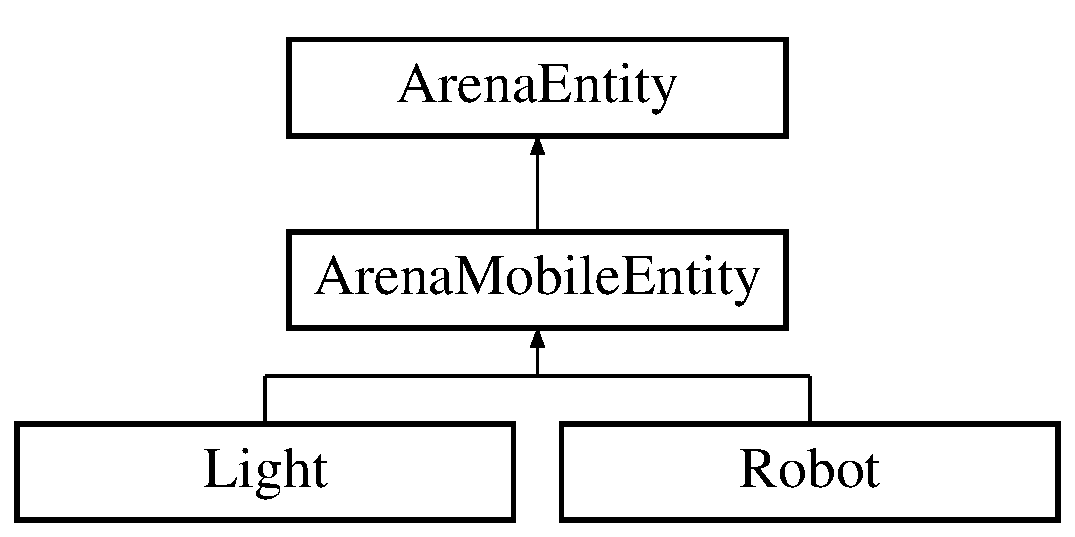
\includegraphics[height=3.000000cm]{class_arena_mobile_entity}
\end{center}
\end{figure}
\subsection*{Public Member Functions}
\begin{DoxyCompactItemize}
\item 
\mbox{\Hypertarget{class_arena_mobile_entity_a6d038ac71d9b149052fc5a0fec4907f9}\label{class_arena_mobile_entity_a6d038ac71d9b149052fc5a0fec4907f9}} 
\mbox{\hyperlink{class_arena_mobile_entity_a6d038ac71d9b149052fc5a0fec4907f9}{Arena\+Mobile\+Entity}} ()
\begin{DoxyCompactList}\small\item\em \mbox{\hyperlink{class_arena_mobile_entity}{Arena\+Mobile\+Entity}}\textquotesingle{}s constructor. \end{DoxyCompactList}\item 
\mbox{\Hypertarget{class_arena_mobile_entity_ad662f3efc1a56b64ecaf5633e7ff2139}\label{class_arena_mobile_entity_ad662f3efc1a56b64ecaf5633e7ff2139}} 
\mbox{\hyperlink{class_arena_mobile_entity_ad662f3efc1a56b64ecaf5633e7ff2139}{Arena\+Mobile\+Entity}} (const \mbox{\hyperlink{class_arena_mobile_entity}{Arena\+Mobile\+Entity}} \&other)=delete
\begin{DoxyCompactList}\small\item\em Under certain circumstance, the compiler requires that the copy constructor is not defined. This {\ttfamily deletes} the default copy constructor. \end{DoxyCompactList}\item 
\mbox{\Hypertarget{class_arena_mobile_entity_a34a7f0d094515cafff7611a0f6cf4eee}\label{class_arena_mobile_entity_a34a7f0d094515cafff7611a0f6cf4eee}} 
\mbox{\hyperlink{class_arena_mobile_entity}{Arena\+Mobile\+Entity}} \& \mbox{\hyperlink{class_arena_mobile_entity_a34a7f0d094515cafff7611a0f6cf4eee}{operator=}} (const \mbox{\hyperlink{class_arena_mobile_entity}{Arena\+Mobile\+Entity}} \&other)=delete
\begin{DoxyCompactList}\small\item\em Under certain circumstance, the compiler requires that the assignment operator is not defined. This {\ttfamily deletes} the default assignment operator. \end{DoxyCompactList}\item 
\mbox{\Hypertarget{class_arena_mobile_entity_a2116341414a3ad0449dc03efa6ea500b}\label{class_arena_mobile_entity_a2116341414a3ad0449dc03efa6ea500b}} 
virtual double \mbox{\hyperlink{class_arena_mobile_entity_a2116341414a3ad0449dc03efa6ea500b}{get\+\_\+speed}} ()
\begin{DoxyCompactList}\small\item\em Returns the speed of the entity. \end{DoxyCompactList}\item 
\mbox{\Hypertarget{class_arena_mobile_entity_a1a047f4377a9557516a2e1d6d73db849}\label{class_arena_mobile_entity_a1a047f4377a9557516a2e1d6d73db849}} 
virtual void \mbox{\hyperlink{class_arena_mobile_entity_a1a047f4377a9557516a2e1d6d73db849}{set\+\_\+speed}} (double sp)
\begin{DoxyCompactList}\small\item\em Sets the speed of the entity. \end{DoxyCompactList}\item 
\mbox{\Hypertarget{class_arena_mobile_entity_ae9507f1b0c6bfdfd62afbab8a9a150f7}\label{class_arena_mobile_entity_ae9507f1b0c6bfdfd62afbab8a9a150f7}} 
\mbox{\hyperlink{class_sensor_touch}{Sensor\+Touch}} $\ast$ \mbox{\hyperlink{class_arena_mobile_entity_ae9507f1b0c6bfdfd62afbab8a9a150f7}{get\+\_\+touch\+\_\+sensor}} ()
\begin{DoxyCompactList}\small\item\em Get a pointer to the \mbox{\hyperlink{class_arena_mobile_entity}{Arena\+Mobile\+Entity}}\textquotesingle{}s touch sensor. \end{DoxyCompactList}\end{DoxyCompactItemize}
\subsection*{Protected Attributes}
\begin{DoxyCompactItemize}
\item 
\mbox{\Hypertarget{class_arena_mobile_entity_a260fd3fba196ee9ab56f9f2ce6ab4a21}\label{class_arena_mobile_entity_a260fd3fba196ee9ab56f9f2ce6ab4a21}} 
\mbox{\hyperlink{class_sensor_touch}{Sensor\+Touch}} $\ast$ {\bfseries sensor\+\_\+touch\+\_\+}
\end{DoxyCompactItemize}


\subsection{Detailed Description}
A mobile entity in the \mbox{\hyperlink{class_arena}{Arena}}, capable of updating its own position and/or velocity when asked by the simulation. 

All mobile entities must have a heading angle so that their orientation can be properly drawn by the \mbox{\hyperlink{class_graphics_arena_viewer}{Graphics\+Arena\+Viewer}}.

Since this is also a food class, many of its methods are intuitively {\ttfamily virtual}. 

The documentation for this class was generated from the following file\+:\begin{DoxyCompactItemize}
\item 
src/\mbox{\hyperlink{arena__mobile__entity_8h}{arena\+\_\+mobile\+\_\+entity.\+h}}\end{DoxyCompactItemize}

\hypertarget{class_braitenberg}{}\section{Braitenberg Class Reference}
\label{class_braitenberg}\index{Braitenberg@{Braitenberg}}


This parent class for all of the possible robot behaviors.  




{\ttfamily \#include $<$braitenberg.\+h$>$}

Inheritance diagram for Braitenberg\+:\begin{figure}[H]
\begin{center}
\leavevmode
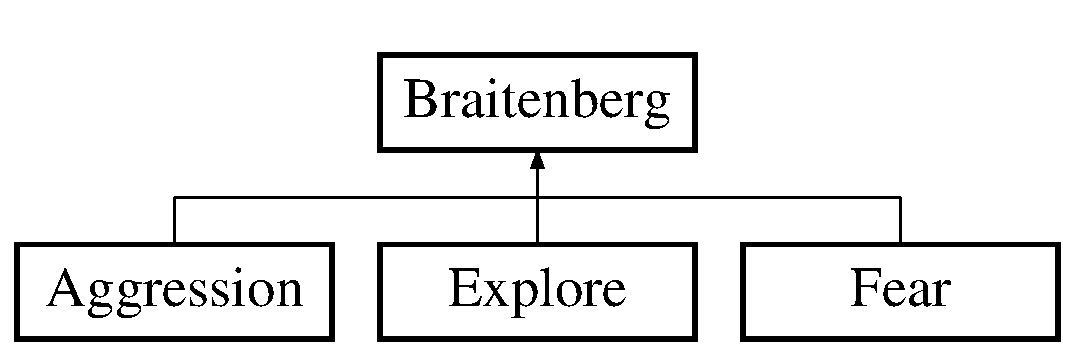
\includegraphics[height=2.000000cm]{class_braitenberg}
\end{center}
\end{figure}
\subsection*{Public Member Functions}
\begin{DoxyCompactItemize}
\item 
\mbox{\Hypertarget{class_braitenberg_a4ee23d8db33e23db109f7f29164d8a23}\label{class_braitenberg_a4ee23d8db33e23db109f7f29164d8a23}} 
\mbox{\hyperlink{class_braitenberg_a4ee23d8db33e23db109f7f29164d8a23}{Braitenberg}} ()
\begin{DoxyCompactList}\small\item\em Empty default constructor. \end{DoxyCompactList}\item 
\mbox{\Hypertarget{class_braitenberg_acd0c15e660bb9d94f6dac077b61cf189}\label{class_braitenberg_acd0c15e660bb9d94f6dac077b61cf189}} 
virtual \mbox{\hyperlink{class_braitenberg_acd0c15e660bb9d94f6dac077b61cf189}{$\sim$\+Braitenberg}} ()
\begin{DoxyCompactList}\small\item\em Empty destructor. \end{DoxyCompactList}\item 
\mbox{\Hypertarget{class_braitenberg_a46af2879438ad5e946f771239f84c308}\label{class_braitenberg_a46af2879438ad5e946f771239f84c308}} 
virtual \mbox{\hyperlink{struct_wheel_velocity}{Wheel\+Velocity}} \mbox{\hyperlink{class_braitenberg_a46af2879438ad5e946f771239f84c308}{Calc\+Wheel\+Velocity}} (\mbox{\hyperlink{common_8h_a2e3484535ee610c8e19e9859563abe48}{\+\_\+\+\_\+unused}} double left\+\_\+reading, \mbox{\hyperlink{common_8h_a2e3484535ee610c8e19e9859563abe48}{\+\_\+\+\_\+unused}} double right\+\_\+reading)
\begin{DoxyCompactList}\small\item\em When overwritten this only takes into account either food or light and returns an appropriate wheel velocity based upon proximity. \end{DoxyCompactList}\item 
\mbox{\Hypertarget{class_braitenberg_af79ef8be83a527368586513773cbd095}\label{class_braitenberg_af79ef8be83a527368586513773cbd095}} 
virtual \mbox{\hyperlink{struct_wheel_velocity}{Wheel\+Velocity}} \mbox{\hyperlink{class_braitenberg_af79ef8be83a527368586513773cbd095}{Calc\+Wheel\+Velocity\+W\+Food}} (\mbox{\hyperlink{common_8h_a2e3484535ee610c8e19e9859563abe48}{\+\_\+\+\_\+unused}} double left\+\_\+light\+\_\+reading, \mbox{\hyperlink{common_8h_a2e3484535ee610c8e19e9859563abe48}{\+\_\+\+\_\+unused}} double right\+\_\+light\+\_\+reading, \mbox{\hyperlink{common_8h_a2e3484535ee610c8e19e9859563abe48}{\+\_\+\+\_\+unused}} double left\+\_\+food\+\_\+reading, \mbox{\hyperlink{common_8h_a2e3484535ee610c8e19e9859563abe48}{\+\_\+\+\_\+unused}} double right\+\_\+food\+\_\+reading)
\begin{DoxyCompactList}\small\item\em Takes into account both the food and the light, returns appropriate wheel velocity. \end{DoxyCompactList}\end{DoxyCompactItemize}


\subsection{Detailed Description}
This parent class for all of the possible robot behaviors. 

The three possible subclasses as of right now are \mbox{\hyperlink{class_fear}{Fear}}, \mbox{\hyperlink{class_aggression}{Aggression}}, \mbox{\hyperlink{class_explore}{Explore}} These classes override the Calc\+Wheel\+Velocity and Calc\+Wheel\+Velocity\+W\+Food methods. Based upon the circumstances this controls the robot\textquotesingle{}s behavior towards food and light. 

The documentation for this class was generated from the following file\+:\begin{DoxyCompactItemize}
\item 
src/\mbox{\hyperlink{braitenberg_8h}{braitenberg.\+h}}\end{DoxyCompactItemize}

\hypertarget{class_controller}{}\section{Controller Class Reference}
\label{class_controller}\index{Controller@{Controller}}


\mbox{\hyperlink{class_controller}{Controller}} that mediates \mbox{\hyperlink{class_arena}{Arena}} and \mbox{\hyperlink{class_graphics_arena_viewer}{Graphics\+Arena\+Viewer}} communication.  




{\ttfamily \#include $<$controller.\+h$>$}

\subsection*{Public Member Functions}
\begin{DoxyCompactItemize}
\item 
\mbox{\Hypertarget{class_controller_a95c56822d667e94b031451729ce069a9}\label{class_controller_a95c56822d667e94b031451729ce069a9}} 
\mbox{\hyperlink{class_controller_a95c56822d667e94b031451729ce069a9}{Controller}} ()
\begin{DoxyCompactList}\small\item\em \mbox{\hyperlink{class_controller}{Controller}}\textquotesingle{}s constructor that will create \mbox{\hyperlink{class_arena}{Arena}} and Viewer. \end{DoxyCompactList}\item 
\mbox{\Hypertarget{class_controller_a17abb2cec6c0109e9b2df3cdc082eaad}\label{class_controller_a17abb2cec6c0109e9b2df3cdc082eaad}} 
void \mbox{\hyperlink{class_controller_a17abb2cec6c0109e9b2df3cdc082eaad}{Run}} ()
\begin{DoxyCompactList}\small\item\em Run launches the graphics and starts the game. \end{DoxyCompactList}\item 
\mbox{\Hypertarget{class_controller_a6a4a3eaee03f6c4718da3f8293d7e053}\label{class_controller_a6a4a3eaee03f6c4718da3f8293d7e053}} 
void \mbox{\hyperlink{class_controller_a6a4a3eaee03f6c4718da3f8293d7e053}{Advance\+Time}} (double dt)
\begin{DoxyCompactList}\small\item\em Advance\+Time is communication from the Viewer to advance the simulation. \end{DoxyCompactList}\item 
\mbox{\Hypertarget{class_controller_a55b8d46984535adb91f40309914e8852}\label{class_controller_a55b8d46984535adb91f40309914e8852}} 
void \mbox{\hyperlink{class_controller_a55b8d46984535adb91f40309914e8852}{Accept\+Communication}} (Communication com)
\begin{DoxyCompactList}\small\item\em Accept\+Communication from either the viewer or the \mbox{\hyperlink{class_arena}{Arena}}. \end{DoxyCompactList}\item 
Communication \mbox{\hyperlink{class_controller_ae9b0504ab74cdacc654528b609074adc}{Convert\+Comm}} (Communication com)
\begin{DoxyCompactList}\small\item\em Converts the communication from one to send to the other. \end{DoxyCompactList}\item 
\mbox{\Hypertarget{class_controller_a9baedd1cbf0bd6fcb771ffda21fafc7b}\label{class_controller_a9baedd1cbf0bd6fcb771ffda21fafc7b}} 
void \mbox{\hyperlink{class_controller_a9baedd1cbf0bd6fcb771ffda21fafc7b}{Change\+Num\+Fear\+Robots}} (int n\+\_\+robots)
\begin{DoxyCompactList}\small\item\em Change number of \mbox{\hyperlink{class_fear}{Fear}} robots in the arena. \end{DoxyCompactList}\item 
\mbox{\Hypertarget{class_controller_a88ae74c37bc5d3ee2eef36d485ff65be}\label{class_controller_a88ae74c37bc5d3ee2eef36d485ff65be}} 
void \mbox{\hyperlink{class_controller_a88ae74c37bc5d3ee2eef36d485ff65be}{Change\+Num\+Explore\+Robots}} (int n\+\_\+robots)
\begin{DoxyCompactList}\small\item\em Change number of \mbox{\hyperlink{class_explore}{Explore}} robots in the arena. \end{DoxyCompactList}\item 
\mbox{\Hypertarget{class_controller_a9952d10da6fbc77b3726b7bb7b6c17d4}\label{class_controller_a9952d10da6fbc77b3726b7bb7b6c17d4}} 
void \mbox{\hyperlink{class_controller_a9952d10da6fbc77b3726b7bb7b6c17d4}{Change\+Num\+Lights}} (int n\+\_\+lights)
\begin{DoxyCompactList}\small\item\em Change number of lights in the arena. \end{DoxyCompactList}\item 
\mbox{\Hypertarget{class_controller_a8bb2a21005f9dead1e847681be25044a}\label{class_controller_a8bb2a21005f9dead1e847681be25044a}} 
void \mbox{\hyperlink{class_controller_a8bb2a21005f9dead1e847681be25044a}{Change\+Num\+Food}} (int n\+\_\+food)
\begin{DoxyCompactList}\small\item\em Change number of food in the arena. \end{DoxyCompactList}\item 
\mbox{\Hypertarget{class_controller_aa6a4db6da624cb5509e745371ac5b8e1}\label{class_controller_aa6a4db6da624cb5509e745371ac5b8e1}} 
void \mbox{\hyperlink{class_controller_aa6a4db6da624cb5509e745371ac5b8e1}{Change\+Sensor\+Sensitivity}} (int sensitivity)
\begin{DoxyCompactList}\small\item\em Change the sensitivity of both the food and light sensors. \end{DoxyCompactList}\end{DoxyCompactItemize}


\subsection{Detailed Description}
\mbox{\hyperlink{class_controller}{Controller}} that mediates \mbox{\hyperlink{class_arena}{Arena}} and \mbox{\hyperlink{class_graphics_arena_viewer}{Graphics\+Arena\+Viewer}} communication. 

The \mbox{\hyperlink{class_controller}{Controller}} instantiates the \mbox{\hyperlink{class_arena}{Arena}} and the \mbox{\hyperlink{class_graphics_arena_viewer}{Graphics\+Arena\+Viewer}}. The viewer contains the main loop that keeps it live, but at each update, the viewer sends a message to the controller to update its time.

Other types of communication between \mbox{\hyperlink{class_arena}{Arena}} and Viewer include\+:
\begin{DoxyItemize}
\item keypresses intercepted by the Viewer.
\item Play/\+Pause/\+New Game user input via the Viewer.
\item Game status from arena to the viewer. 
\end{DoxyItemize}

\subsection{Member Function Documentation}
\mbox{\Hypertarget{class_controller_ae9b0504ab74cdacc654528b609074adc}\label{class_controller_ae9b0504ab74cdacc654528b609074adc}} 
\index{Controller@{Controller}!Convert\+Comm@{Convert\+Comm}}
\index{Convert\+Comm@{Convert\+Comm}!Controller@{Controller}}
\subsubsection{\texorpdfstring{Convert\+Comm()}{ConvertComm()}}
{\footnotesize\ttfamily Communication Controller\+::\+Convert\+Comm (\begin{DoxyParamCaption}\item[{Communication}]{com }\end{DoxyParamCaption})}



Converts the communication from one to send to the other. 

Used primarily for testing purposes to insure communication is being correctly received, interpreted, and relayed.

Converts communication from one source to appropriate communication to the other source. For example, the viewer sends a k\+Key\+Up communication, and this translate to a k\+Increase\+Speed communication to \mbox{\hyperlink{class_arena}{Arena}}. \+: Complete the conversion code for all key presses. 

The documentation for this class was generated from the following files\+:\begin{DoxyCompactItemize}
\item 
src/\mbox{\hyperlink{controller_8h}{controller.\+h}}\item 
src/\mbox{\hyperlink{controller_8cc}{controller.\+cc}}\end{DoxyCompactItemize}

\hypertarget{class_entity_factory}{}\section{Entity\+Factory Class Reference}
\label{class_entity_factory}\index{Entity\+Factory@{Entity\+Factory}}


A factory for the instantiation of all types of arena entities.  




{\ttfamily \#include $<$entity\+\_\+factory.\+h$>$}

\subsection*{Public Member Functions}
\begin{DoxyCompactItemize}
\item 
\mbox{\Hypertarget{class_entity_factory_abaf0c4ceaa682e55f69b0ceae230008a}\label{class_entity_factory_abaf0c4ceaa682e55f69b0ceae230008a}} 
\mbox{\hyperlink{class_entity_factory_abaf0c4ceaa682e55f69b0ceae230008a}{Entity\+Factory}} ()
\begin{DoxyCompactList}\small\item\em \mbox{\hyperlink{class_entity_factory}{Entity\+Factory}} constructor. \end{DoxyCompactList}\item 
\mbox{\Hypertarget{class_entity_factory_ae3246f06fa101178803f76582323d4ad}\label{class_entity_factory_ae3246f06fa101178803f76582323d4ad}} 
virtual \mbox{\hyperlink{class_entity_factory_ae3246f06fa101178803f76582323d4ad}{$\sim$\+Entity\+Factory}} ()=default
\begin{DoxyCompactList}\small\item\em Default destructor. \end{DoxyCompactList}\item 
\mbox{\hyperlink{class_arena_entity}{Arena\+Entity}} $\ast$ \mbox{\hyperlink{class_entity_factory_af8366cb210cfb13f94b8eeb502e805fc}{Create\+Entity}} (Entity\+Type etype, Behavior behavior)
\begin{DoxyCompactList}\small\item\em Create\+Entity is primary purpose of this class. \end{DoxyCompactList}\item 
\mbox{\Hypertarget{class_entity_factory_a8c419808ccf0f71fb35ac77eed30fc30}\label{class_entity_factory_a8c419808ccf0f71fb35ac77eed30fc30}} 
int {\bfseries get\+\_\+entity\+\_\+count} ()
\item 
\mbox{\Hypertarget{class_entity_factory_a51a6685d0a6d529f1b3ea7538fa2fb97}\label{class_entity_factory_a51a6685d0a6d529f1b3ea7538fa2fb97}} 
void {\bfseries set\+\_\+entity\+\_\+count} (int entity\+\_\+count)
\item 
\mbox{\Hypertarget{class_entity_factory_acc8d2184f834fe2f663fea781b6aba80}\label{class_entity_factory_acc8d2184f834fe2f663fea781b6aba80}} 
int {\bfseries get\+\_\+robot\+\_\+count} ()
\item 
\mbox{\Hypertarget{class_entity_factory_abdb8ab57e9a0faa3ce2add10da2380e7}\label{class_entity_factory_abdb8ab57e9a0faa3ce2add10da2380e7}} 
void {\bfseries set\+\_\+robot\+\_\+count} (int robot\+\_\+count)
\item 
\mbox{\Hypertarget{class_entity_factory_a6e949ab2d1b1dc788715889a881c08b2}\label{class_entity_factory_a6e949ab2d1b1dc788715889a881c08b2}} 
int {\bfseries get\+\_\+light\+\_\+count} ()
\item 
\mbox{\Hypertarget{class_entity_factory_a087936314af6334242d270cda1bf8209}\label{class_entity_factory_a087936314af6334242d270cda1bf8209}} 
void {\bfseries set\+\_\+light\+\_\+count} (int light\+\_\+count)
\item 
\mbox{\Hypertarget{class_entity_factory_ad70396eb638676d5a833be3327f62554}\label{class_entity_factory_ad70396eb638676d5a833be3327f62554}} 
int {\bfseries get\+\_\+food\+\_\+count} ()
\item 
\mbox{\Hypertarget{class_entity_factory_ab1097be73754ac0aa8debb680c216e9d}\label{class_entity_factory_ab1097be73754ac0aa8debb680c216e9d}} 
void {\bfseries set\+\_\+food\+\_\+count} (int food\+\_\+count)
\end{DoxyCompactItemize}


\subsection{Detailed Description}
A factory for the instantiation of all types of arena entities. 

The factory keeps track of the number of entities of each type and overall. It assigns ID\textquotesingle{}s to the entity when it creates it. The factory randomly places entities, and in doing so, attempts to not have them overlap. 

\subsection{Member Function Documentation}
\mbox{\Hypertarget{class_entity_factory_af8366cb210cfb13f94b8eeb502e805fc}\label{class_entity_factory_af8366cb210cfb13f94b8eeb502e805fc}} 
\index{Entity\+Factory@{Entity\+Factory}!Create\+Entity@{Create\+Entity}}
\index{Create\+Entity@{Create\+Entity}!Entity\+Factory@{Entity\+Factory}}
\subsubsection{\texorpdfstring{Create\+Entity()}{CreateEntity()}}
{\footnotesize\ttfamily \mbox{\hyperlink{class_arena_entity}{Arena\+Entity}} $\ast$ Entity\+Factory\+::\+Create\+Entity (\begin{DoxyParamCaption}\item[{Entity\+Type}]{etype,  }\item[{Behavior}]{behavior }\end{DoxyParamCaption})}



Create\+Entity is primary purpose of this class. 


\begin{DoxyParams}[1]{Parameters}
\mbox{\tt in}  & {\em etype} & The type to make. \\
\hline
\mbox{\tt in}  & {\em behavior,in} & case it is a robot \\
\hline
\mbox{\tt out}  & {\em new} & dynamically created entity.\\
\hline
\end{DoxyParams}
Currently, the \mbox{\hyperlink{class_arena}{Arena}} gets the entity and places it in the appropriate data structure. It might be useful to instead have the factory place on the appropriate data structure so that the call to \mbox{\hyperlink{class_arena}{Arena}} is the same regardless of the entity type. 

The documentation for this class was generated from the following files\+:\begin{DoxyCompactItemize}
\item 
src/\mbox{\hyperlink{entity__factory_8h}{entity\+\_\+factory.\+h}}\item 
src/\mbox{\hyperlink{entity__factory_8cc}{entity\+\_\+factory.\+cc}}\end{DoxyCompactItemize}

\hypertarget{class_explore}{}\section{Explore Class Reference}
\label{class_explore}\index{Explore@{Explore}}


The class for the robot explore behavior.  




{\ttfamily \#include $<$explore.\+h$>$}

Inheritance diagram for Explore\+:\begin{figure}[H]
\begin{center}
\leavevmode
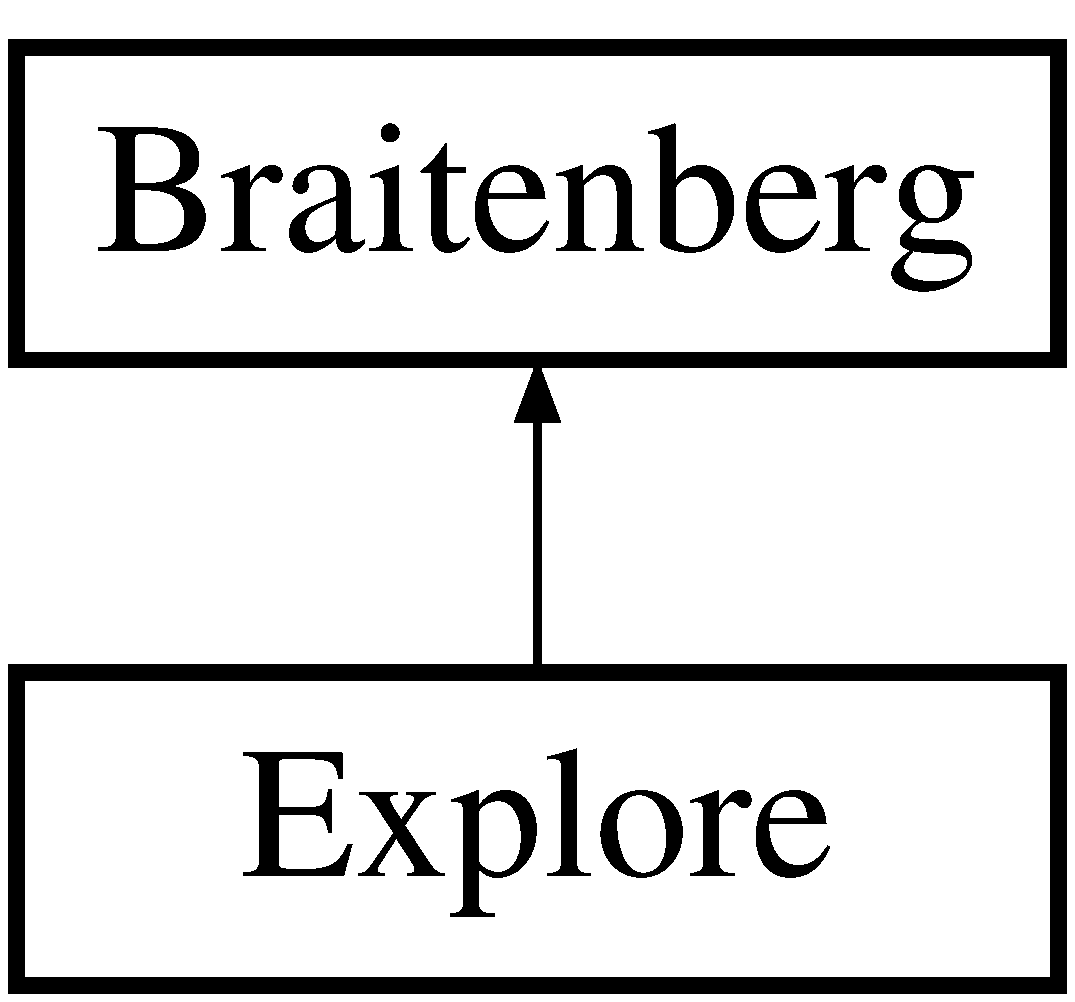
\includegraphics[height=2.000000cm]{class_explore}
\end{center}
\end{figure}
\subsection*{Public Member Functions}
\begin{DoxyCompactItemize}
\item 
\mbox{\Hypertarget{class_explore_a8ace99bb96956cb6b4c7d4e32923a843}\label{class_explore_a8ace99bb96956cb6b4c7d4e32923a843}} 
\mbox{\hyperlink{class_explore_a8ace99bb96956cb6b4c7d4e32923a843}{Explore}} ()
\begin{DoxyCompactList}\small\item\em Empty default constructor. \end{DoxyCompactList}\item 
\mbox{\Hypertarget{class_explore_a0ef9a84d8be98aedc05cbd05232c4095}\label{class_explore_a0ef9a84d8be98aedc05cbd05232c4095}} 
virtual \mbox{\hyperlink{class_explore_a0ef9a84d8be98aedc05cbd05232c4095}{$\sim$\+Explore}} ()=default
\begin{DoxyCompactList}\small\item\em Default destructors. \end{DoxyCompactList}\item 
\mbox{\hyperlink{struct_wheel_velocity}{Wheel\+Velocity}} \mbox{\hyperlink{class_explore_aae196c161cfab6179cb7c93722c44937}{Calc\+Wheel\+Velocity}} (double left\+\_\+reading, double right\+\_\+reading) override
\begin{DoxyCompactList}\small\item\em Determine the speed of both wheels based upon the robots proximity to the light. \end{DoxyCompactList}\item 
\mbox{\hyperlink{struct_wheel_velocity}{Wheel\+Velocity}} \mbox{\hyperlink{class_explore_aee6c025989c1aef2c76ccaa3db61ace1}{Calc\+Wheel\+Velocity\+W\+Food}} (double left\+\_\+light\+\_\+reading, double right\+\_\+light\+\_\+reading, double left\+\_\+food\+\_\+reading, double right\+\_\+food\+\_\+reading) override
\begin{DoxyCompactList}\small\item\em Determine the speed of both wheels based upon the robots proximity to the food and the light. \end{DoxyCompactList}\end{DoxyCompactItemize}


\subsection{Detailed Description}
The class for the robot explore behavior. 

This class inherits from \mbox{\hyperlink{class_braitenberg}{Braitenberg}} and overrides its Calc\+Wheel\+Velocity and Calc\+Wheel\+Velocity\+W\+Food methods. The robot will move quick and avoid light 

\subsection{Member Function Documentation}
\mbox{\Hypertarget{class_explore_aae196c161cfab6179cb7c93722c44937}\label{class_explore_aae196c161cfab6179cb7c93722c44937}} 
\index{Explore@{Explore}!Calc\+Wheel\+Velocity@{Calc\+Wheel\+Velocity}}
\index{Calc\+Wheel\+Velocity@{Calc\+Wheel\+Velocity}!Explore@{Explore}}
\subsubsection{\texorpdfstring{Calc\+Wheel\+Velocity()}{CalcWheelVelocity()}}
{\footnotesize\ttfamily \mbox{\hyperlink{struct_wheel_velocity}{Wheel\+Velocity}} Explore\+::\+Calc\+Wheel\+Velocity (\begin{DoxyParamCaption}\item[{double}]{left\+\_\+reading,  }\item[{double}]{right\+\_\+reading }\end{DoxyParamCaption})\hspace{0.3cm}{\ttfamily [override]}}



Determine the speed of both wheels based upon the robots proximity to the light. 


\begin{DoxyParams}[1]{Parameters}
\mbox{\tt in}  & {\em left\+\_\+reading} & -\/ reading for light sensor on the left \\
\hline
\mbox{\tt in}  & {\em right\+\_\+reading} & -\/ reading for light sensor on the right \\
\hline
\mbox{\tt out}  & {\em The} & proper wheel velocities \\
\hline
\end{DoxyParams}
\mbox{\Hypertarget{class_explore_aee6c025989c1aef2c76ccaa3db61ace1}\label{class_explore_aee6c025989c1aef2c76ccaa3db61ace1}} 
\index{Explore@{Explore}!Calc\+Wheel\+Velocity\+W\+Food@{Calc\+Wheel\+Velocity\+W\+Food}}
\index{Calc\+Wheel\+Velocity\+W\+Food@{Calc\+Wheel\+Velocity\+W\+Food}!Explore@{Explore}}
\subsubsection{\texorpdfstring{Calc\+Wheel\+Velocity\+W\+Food()}{CalcWheelVelocityWFood()}}
{\footnotesize\ttfamily \mbox{\hyperlink{struct_wheel_velocity}{Wheel\+Velocity}} Explore\+::\+Calc\+Wheel\+Velocity\+W\+Food (\begin{DoxyParamCaption}\item[{double}]{left\+\_\+light\+\_\+reading,  }\item[{double}]{right\+\_\+light\+\_\+reading,  }\item[{double}]{left\+\_\+food\+\_\+reading,  }\item[{double}]{right\+\_\+food\+\_\+reading }\end{DoxyParamCaption})\hspace{0.3cm}{\ttfamily [override]}}



Determine the speed of both wheels based upon the robots proximity to the food and the light. 


\begin{DoxyParams}[1]{Parameters}
\mbox{\tt in}  & {\em left\+\_\+light\+\_\+reading} & -\/ reading for light sensor on the left \\
\hline
\mbox{\tt in}  & {\em right\+\_\+light\+\_\+reading} & -\/ reading for light sensor on the right \\
\hline
\mbox{\tt in}  & {\em left\+\_\+food\+\_\+reading} & -\/ reading for food sensor on the left \\
\hline
\mbox{\tt in}  & {\em right\+\_\+food\+\_\+reading} & -\/ reading for food sensor on the right \\
\hline
\mbox{\tt out}  & {\em The} & proper wheel velocities \\
\hline
\end{DoxyParams}


The documentation for this class was generated from the following files\+:\begin{DoxyCompactItemize}
\item 
src/\mbox{\hyperlink{explore_8h}{explore.\+h}}\item 
src/\mbox{\hyperlink{explore_8cc}{explore.\+cc}}\end{DoxyCompactItemize}

\hypertarget{class_fear}{}\section{Fear Class Reference}
\label{class_fear}\index{Fear@{Fear}}


The class for the robot fear behavior.  




{\ttfamily \#include $<$fear.\+h$>$}

Inheritance diagram for Fear\+:\begin{figure}[H]
\begin{center}
\leavevmode
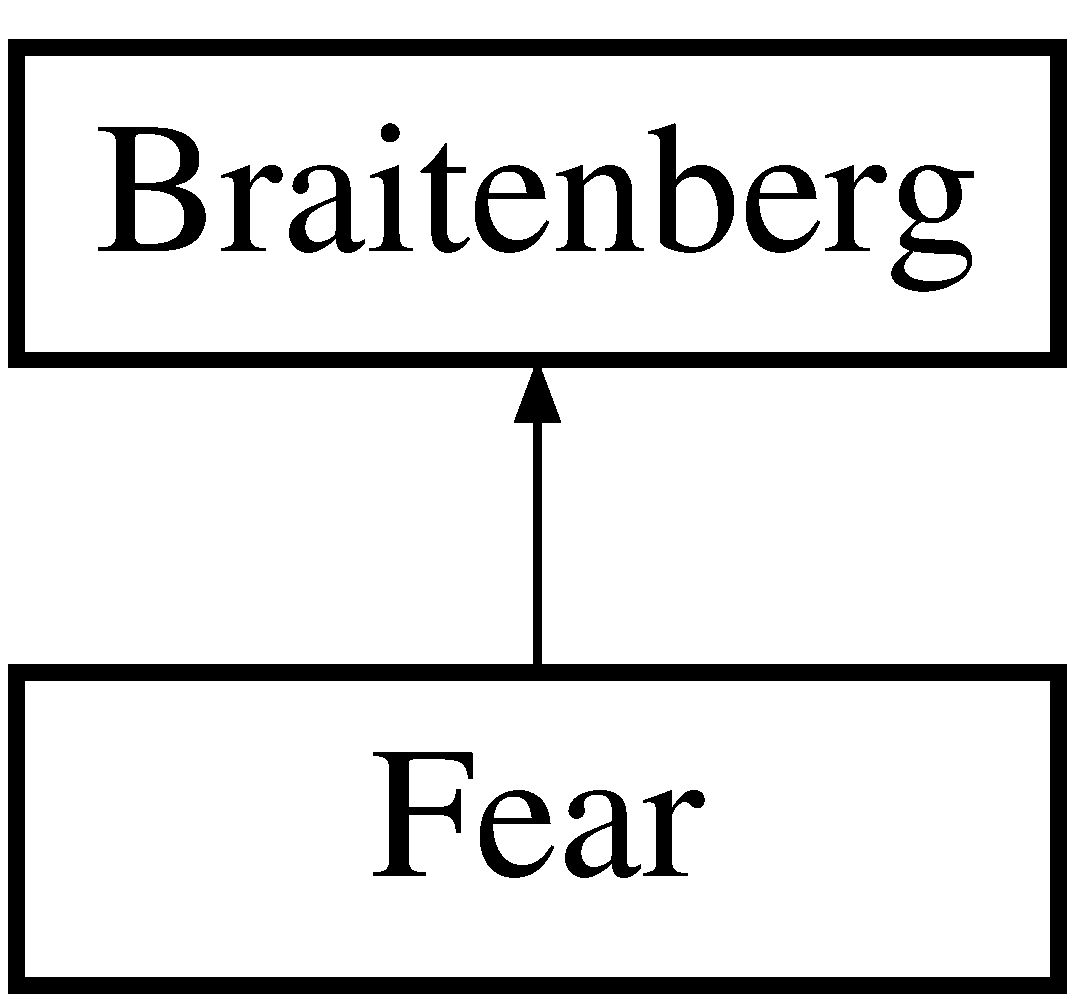
\includegraphics[height=2.000000cm]{class_fear}
\end{center}
\end{figure}
\subsection*{Public Member Functions}
\begin{DoxyCompactItemize}
\item 
\mbox{\Hypertarget{class_fear_a2a7cfce798f1b86f73510a62232975f8}\label{class_fear_a2a7cfce798f1b86f73510a62232975f8}} 
\mbox{\hyperlink{class_fear_a2a7cfce798f1b86f73510a62232975f8}{Fear}} ()
\begin{DoxyCompactList}\small\item\em Empty default constructor. \end{DoxyCompactList}\item 
\mbox{\Hypertarget{class_fear_a571e48276ff3e227caf1d2d3445ed100}\label{class_fear_a571e48276ff3e227caf1d2d3445ed100}} 
virtual \mbox{\hyperlink{class_fear_a571e48276ff3e227caf1d2d3445ed100}{$\sim$\+Fear}} ()=default
\begin{DoxyCompactList}\small\item\em Default destructors. \end{DoxyCompactList}\item 
\mbox{\hyperlink{struct_wheel_velocity}{Wheel\+Velocity}} \mbox{\hyperlink{class_fear_a17242c34a557281ad98d37073f590c45}{Calc\+Wheel\+Velocity}} (double left\+\_\+reading, double right\+\_\+reading) override
\begin{DoxyCompactList}\small\item\em Determine the speed of both wheels based upon the robots proximity to the light. \end{DoxyCompactList}\item 
\mbox{\hyperlink{struct_wheel_velocity}{Wheel\+Velocity}} \mbox{\hyperlink{class_fear_a24a9b3c3dec205cb973eb15416795129}{Calc\+Wheel\+Velocity\+W\+Food}} (double left\+\_\+light\+\_\+reading, double right\+\_\+light\+\_\+reading, double left\+\_\+food\+\_\+reading, double right\+\_\+food\+\_\+reading) override
\begin{DoxyCompactList}\small\item\em Determine the speed of both wheels based upon the robots proximity to the food and the light. \end{DoxyCompactList}\end{DoxyCompactItemize}


\subsection{Detailed Description}
The class for the robot fear behavior. 

This class inherits from \mbox{\hyperlink{class_braitenberg}{Braitenberg}} and overrides its Calc\+Wheel\+Velocity and Calc\+Wheel\+Velocity\+W\+Food methods. The robot will move slowly and avoid light when it is near 

\subsection{Member Function Documentation}
\mbox{\Hypertarget{class_fear_a17242c34a557281ad98d37073f590c45}\label{class_fear_a17242c34a557281ad98d37073f590c45}} 
\index{Fear@{Fear}!Calc\+Wheel\+Velocity@{Calc\+Wheel\+Velocity}}
\index{Calc\+Wheel\+Velocity@{Calc\+Wheel\+Velocity}!Fear@{Fear}}
\subsubsection{\texorpdfstring{Calc\+Wheel\+Velocity()}{CalcWheelVelocity()}}
{\footnotesize\ttfamily \mbox{\hyperlink{struct_wheel_velocity}{Wheel\+Velocity}} Fear\+::\+Calc\+Wheel\+Velocity (\begin{DoxyParamCaption}\item[{double}]{left\+\_\+reading,  }\item[{double}]{right\+\_\+reading }\end{DoxyParamCaption})\hspace{0.3cm}{\ttfamily [override]}}



Determine the speed of both wheels based upon the robots proximity to the light. 


\begin{DoxyParams}[1]{Parameters}
\mbox{\tt in}  & {\em left\+\_\+reading} & -\/ reading for light sensor on the left \\
\hline
\mbox{\tt in}  & {\em right\+\_\+reading} & -\/ reading for light sensor on the right \\
\hline
\mbox{\tt out}  & {\em The} & proper wheel velocities \\
\hline
\end{DoxyParams}
\mbox{\Hypertarget{class_fear_a24a9b3c3dec205cb973eb15416795129}\label{class_fear_a24a9b3c3dec205cb973eb15416795129}} 
\index{Fear@{Fear}!Calc\+Wheel\+Velocity\+W\+Food@{Calc\+Wheel\+Velocity\+W\+Food}}
\index{Calc\+Wheel\+Velocity\+W\+Food@{Calc\+Wheel\+Velocity\+W\+Food}!Fear@{Fear}}
\subsubsection{\texorpdfstring{Calc\+Wheel\+Velocity\+W\+Food()}{CalcWheelVelocityWFood()}}
{\footnotesize\ttfamily \mbox{\hyperlink{struct_wheel_velocity}{Wheel\+Velocity}} Fear\+::\+Calc\+Wheel\+Velocity\+W\+Food (\begin{DoxyParamCaption}\item[{double}]{left\+\_\+light\+\_\+reading,  }\item[{double}]{right\+\_\+light\+\_\+reading,  }\item[{double}]{left\+\_\+food\+\_\+reading,  }\item[{double}]{right\+\_\+food\+\_\+reading }\end{DoxyParamCaption})\hspace{0.3cm}{\ttfamily [override]}}



Determine the speed of both wheels based upon the robots proximity to the food and the light. 


\begin{DoxyParams}[1]{Parameters}
\mbox{\tt in}  & {\em left\+\_\+light\+\_\+reading} & -\/ reading for light sensor on the left \\
\hline
\mbox{\tt in}  & {\em right\+\_\+light\+\_\+reading} & -\/ reading for light sensor on the right \\
\hline
\mbox{\tt in}  & {\em left\+\_\+food\+\_\+reading} & -\/ reading for food sensor on the left \\
\hline
\mbox{\tt in}  & {\em right\+\_\+food\+\_\+reading} & -\/ reading for food sensor on the right \\
\hline
\mbox{\tt out}  & {\em The} & proper wheel velocities \\
\hline
\end{DoxyParams}


The documentation for this class was generated from the following files\+:\begin{DoxyCompactItemize}
\item 
src/\mbox{\hyperlink{fear_8h}{fear.\+h}}\item 
src/\mbox{\hyperlink{fear_8cc}{fear.\+cc}}\end{DoxyCompactItemize}

\hypertarget{class_food}{}\section{Food Class Reference}
\label{class_food}\index{Food@{Food}}


Class representing a immobile food within the \mbox{\hyperlink{class_arena}{Arena}}.  




{\ttfamily \#include $<$food.\+h$>$}

Inheritance diagram for Food\+:\begin{figure}[H]
\begin{center}
\leavevmode
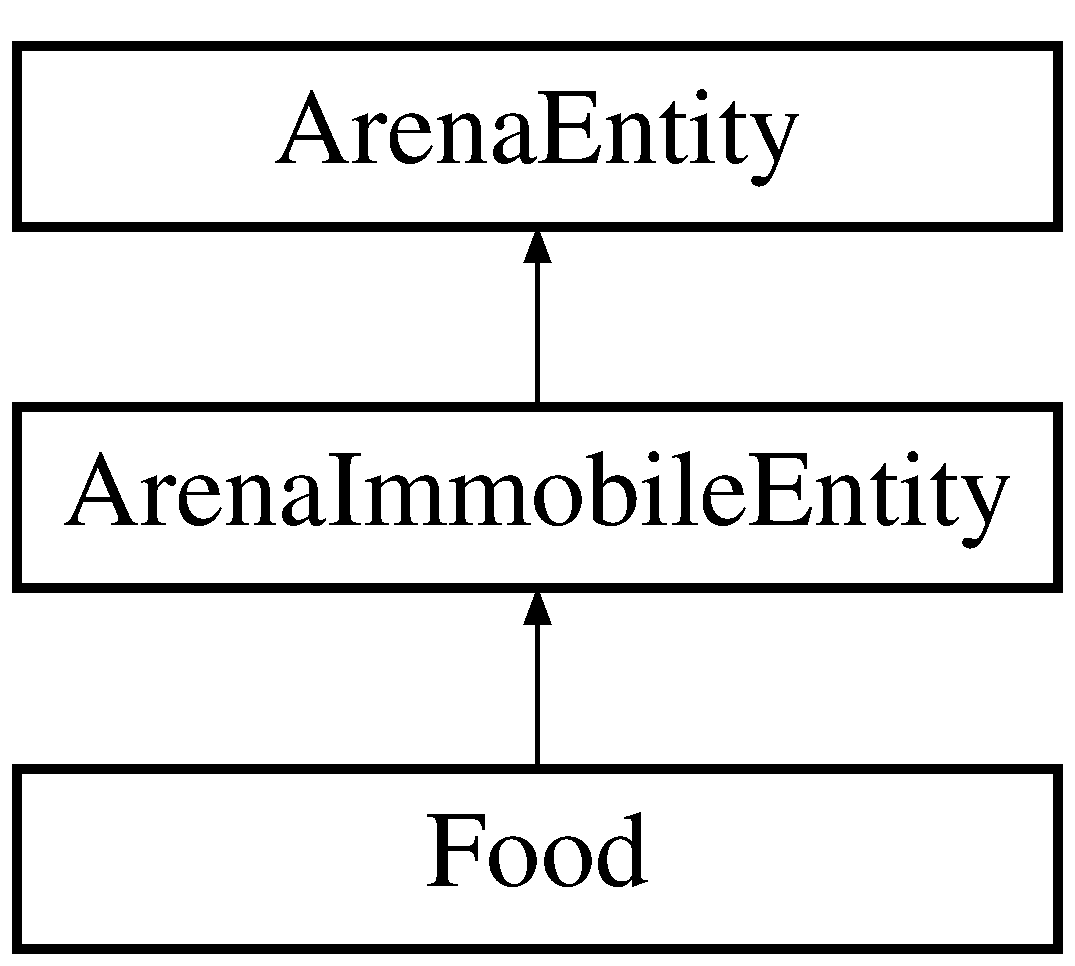
\includegraphics[height=3.000000cm]{class_food}
\end{center}
\end{figure}
\subsection*{Public Member Functions}
\begin{DoxyCompactItemize}
\item 
\mbox{\hyperlink{class_food_a75d4d7f76fd495cc8133302ca9fdc485}{Food}} ()
\begin{DoxyCompactList}\small\item\em Constructor. \end{DoxyCompactList}\item 
\mbox{\Hypertarget{class_food_a1a12bfd50400e04b595c24a512317c1a}\label{class_food_a1a12bfd50400e04b595c24a512317c1a}} 
void \mbox{\hyperlink{class_food_a1a12bfd50400e04b595c24a512317c1a}{Reset}} () override
\begin{DoxyCompactList}\small\item\em Reset the \mbox{\hyperlink{class_food}{Food}} using the initialization parameters received by the constructor. \end{DoxyCompactList}\item 
std\+::string \mbox{\hyperlink{class_food_a5c3bcd5109750a15ebb24b8a2a3cdd07}{get\+\_\+name}} () const override
\begin{DoxyCompactList}\small\item\em Get the name of the \mbox{\hyperlink{class_food}{Food}} for visualization purposes, and to aid in debugging. \end{DoxyCompactList}\item 
bool \mbox{\hyperlink{class_food_a81c160e9e591b4a4eb9662efb7130ee8}{Is\+Captured}} () const
\begin{DoxyCompactList}\small\item\em Getter for captured\+\_\+, which is the state of the food. \end{DoxyCompactList}\item 
\mbox{\Hypertarget{class_food_a1ad8a3c17f9ab764215320ec11c7c40d}\label{class_food_a1ad8a3c17f9ab764215320ec11c7c40d}} 
void \mbox{\hyperlink{class_food_a1ad8a3c17f9ab764215320ec11c7c40d}{set\+\_\+captured}} (bool state)
\begin{DoxyCompactList}\small\item\em Setter for captured\+\_\+, which is the state of the food. \end{DoxyCompactList}\end{DoxyCompactItemize}


\subsection{Detailed Description}
Class representing a immobile food within the \mbox{\hyperlink{class_arena}{Arena}}. 

\mbox{\hyperlink{class_food}{Food}} can enhance a \mbox{\hyperlink{class_robot}{Robot}}. If a \mbox{\hyperlink{class_robot}{Robot}} touches the \mbox{\hyperlink{class_food}{Food}}, it becomes a super robot.

\mbox{\hyperlink{class_food}{Food}} have the capability of updating their own position when asked, and also track their own velocity and heading. They have a touch sensor for responding to collision events which is activated/deactivated on collision events. 

\subsection{Constructor \& Destructor Documentation}
\mbox{\Hypertarget{class_food_a75d4d7f76fd495cc8133302ca9fdc485}\label{class_food_a75d4d7f76fd495cc8133302ca9fdc485}} 
\index{Food@{Food}!Food@{Food}}
\index{Food@{Food}!Food@{Food}}
\subsubsection{\texorpdfstring{Food()}{Food()}}
{\footnotesize\ttfamily Food\+::\+Food (\begin{DoxyParamCaption}{ }\end{DoxyParamCaption})}



Constructor. 


\begin{DoxyParams}{Parameters}
{\em params} & A food\+\_\+params passed down from \mbox{\hyperlink{main_8cc}{main.\+cc}} for the initialization of the \mbox{\hyperlink{class_food}{Food}}. \\
\hline
\end{DoxyParams}


\subsection{Member Function Documentation}
\mbox{\Hypertarget{class_food_a5c3bcd5109750a15ebb24b8a2a3cdd07}\label{class_food_a5c3bcd5109750a15ebb24b8a2a3cdd07}} 
\index{Food@{Food}!get\+\_\+name@{get\+\_\+name}}
\index{get\+\_\+name@{get\+\_\+name}!Food@{Food}}
\subsubsection{\texorpdfstring{get\+\_\+name()}{get\_name()}}
{\footnotesize\ttfamily std\+::string Food\+::get\+\_\+name (\begin{DoxyParamCaption}{ }\end{DoxyParamCaption}) const\hspace{0.3cm}{\ttfamily [inline]}, {\ttfamily [override]}, {\ttfamily [virtual]}}



Get the name of the \mbox{\hyperlink{class_food}{Food}} for visualization purposes, and to aid in debugging. 

\begin{DoxyReturn}{Returns}
Name of the \mbox{\hyperlink{class_food}{Food}}. 
\end{DoxyReturn}


Implements \mbox{\hyperlink{class_arena_entity_ad43152003033cf01ad86eeff1990b69a}{Arena\+Entity}}.

\mbox{\Hypertarget{class_food_a81c160e9e591b4a4eb9662efb7130ee8}\label{class_food_a81c160e9e591b4a4eb9662efb7130ee8}} 
\index{Food@{Food}!Is\+Captured@{Is\+Captured}}
\index{Is\+Captured@{Is\+Captured}!Food@{Food}}
\subsubsection{\texorpdfstring{Is\+Captured()}{IsCaptured()}}
{\footnotesize\ttfamily bool Food\+::\+Is\+Captured (\begin{DoxyParamCaption}{ }\end{DoxyParamCaption}) const\hspace{0.3cm}{\ttfamily [inline]}}



Getter for captured\+\_\+, which is the state of the food. 

\begin{DoxyReturn}{Returns}
true if captured. 
\end{DoxyReturn}


The documentation for this class was generated from the following files\+:\begin{DoxyCompactItemize}
\item 
src/\mbox{\hyperlink{food_8h}{food.\+h}}\item 
src/\mbox{\hyperlink{food_8cc}{food.\+cc}}\end{DoxyCompactItemize}

\hypertarget{class_food_sensor}{}\section{Food\+Sensor Class Reference}
\label{class_food_sensor}\index{Food\+Sensor@{Food\+Sensor}}


Class representing a food sensor for the robot.  




{\ttfamily \#include $<$food\+\_\+sensor.\+h$>$}

Inheritance diagram for Food\+Sensor\+:\begin{figure}[H]
\begin{center}
\leavevmode
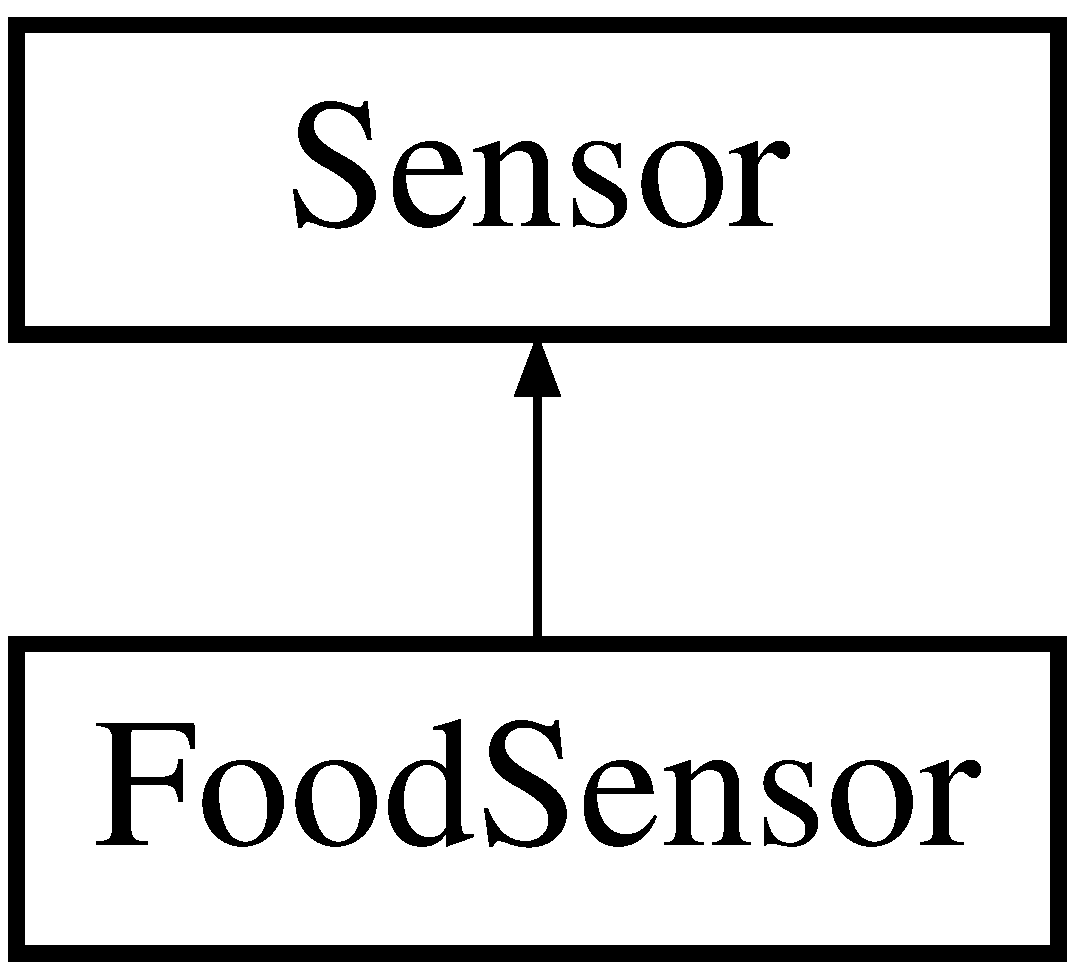
\includegraphics[height=2.000000cm]{class_food_sensor}
\end{center}
\end{figure}
\subsection*{Public Member Functions}
\begin{DoxyCompactItemize}
\item 
\mbox{\hyperlink{class_food_sensor_a80bc0b7b4d46a87a50c0d0094169c9f9}{Food\+Sensor}} (\mbox{\hyperlink{class_robot}{Robot}} $\ast$robot, double sensor\+\_\+angle)
\begin{DoxyCompactList}\small\item\em Constructor. \end{DoxyCompactList}\item 
\mbox{\Hypertarget{class_food_sensor_a749728b0e8179cac51323f9a15750dc3}\label{class_food_sensor_a749728b0e8179cac51323f9a15750dc3}} 
\mbox{\hyperlink{class_food_sensor_a749728b0e8179cac51323f9a15750dc3}{$\sim$\+Food\+Sensor}} ()=default
\begin{DoxyCompactList}\small\item\em Default destructor. \end{DoxyCompactList}\item 
void \mbox{\hyperlink{class_food_sensor_a9220e06a42f2f8385d308a2c88303416}{Notify}} (\mbox{\hyperlink{struct_pose}{Pose}} entity\+\_\+pose) override
\begin{DoxyCompactList}\small\item\em Gives a sensor reading based upon the position passed in. \end{DoxyCompactList}\item 
\mbox{\Hypertarget{class_food_sensor_a1b60ca32e66f68f2ca7ddd1d6d709764}\label{class_food_sensor_a1b60ca32e66f68f2ca7ddd1d6d709764}} 
void \mbox{\hyperlink{class_food_sensor_a1b60ca32e66f68f2ca7ddd1d6d709764}{Reset}} () override
\begin{DoxyCompactList}\small\item\em Resets the position and the sensor reading. \end{DoxyCompactList}\end{DoxyCompactItemize}
\subsection*{Additional Inherited Members}


\subsection{Detailed Description}
Class representing a food sensor for the robot. 

Food\+Sensors are what detect the proximity of the robot to the food. They make sure the robot does not starve

The Food\+Sensors get notified by food and create readings based upon their proximity to the food. 

\subsection{Constructor \& Destructor Documentation}
\mbox{\Hypertarget{class_food_sensor_a80bc0b7b4d46a87a50c0d0094169c9f9}\label{class_food_sensor_a80bc0b7b4d46a87a50c0d0094169c9f9}} 
\index{Food\+Sensor@{Food\+Sensor}!Food\+Sensor@{Food\+Sensor}}
\index{Food\+Sensor@{Food\+Sensor}!Food\+Sensor@{Food\+Sensor}}
\subsubsection{\texorpdfstring{Food\+Sensor()}{FoodSensor()}}
{\footnotesize\ttfamily Food\+Sensor\+::\+Food\+Sensor (\begin{DoxyParamCaption}\item[{\mbox{\hyperlink{class_robot}{Robot}} $\ast$}]{robot,  }\item[{double}]{sensor\+\_\+angle }\end{DoxyParamCaption})}



Constructor. 


\begin{DoxyParams}[1]{Parameters}
\mbox{\tt in}  & {\em robot} & -\/ reference to the robot of this sensor \\
\hline
\mbox{\tt in}  & {\em sensor\+\_\+angle} & -\/ the location of the sensor \\
\hline
\end{DoxyParams}


\subsection{Member Function Documentation}
\mbox{\Hypertarget{class_food_sensor_a9220e06a42f2f8385d308a2c88303416}\label{class_food_sensor_a9220e06a42f2f8385d308a2c88303416}} 
\index{Food\+Sensor@{Food\+Sensor}!Notify@{Notify}}
\index{Notify@{Notify}!Food\+Sensor@{Food\+Sensor}}
\subsubsection{\texorpdfstring{Notify()}{Notify()}}
{\footnotesize\ttfamily void Food\+Sensor\+::\+Notify (\begin{DoxyParamCaption}\item[{\mbox{\hyperlink{struct_pose}{Pose}}}]{entity\+\_\+pose }\end{DoxyParamCaption})\hspace{0.3cm}{\ttfamily [override]}}



Gives a sensor reading based upon the position passed in. 


\begin{DoxyParams}{Parameters}
{\em entity\+\_\+pose} & -\/ the entity to base the reading off of \\
\hline
\end{DoxyParams}


The documentation for this class was generated from the following files\+:\begin{DoxyCompactItemize}
\item 
src/\mbox{\hyperlink{food__sensor_8h}{food\+\_\+sensor.\+h}}\item 
src/food\+\_\+sensor.\+cc\end{DoxyCompactItemize}

\hypertarget{class_graphics_arena_viewer}{}\section{Graphics\+Arena\+Viewer Class Reference}
\label{class_graphics_arena_viewer}\index{Graphics\+Arena\+Viewer@{Graphics\+Arena\+Viewer}}


An application that uses the Min\+Gfx library to open up a window that includes a few buttons for controlling the simulation and can be used to draw circles and other computer graphics.  




{\ttfamily \#include $<$graphics\+\_\+arena\+\_\+viewer.\+h$>$}

Inheritance diagram for Graphics\+Arena\+Viewer\+:\begin{figure}[H]
\begin{center}
\leavevmode
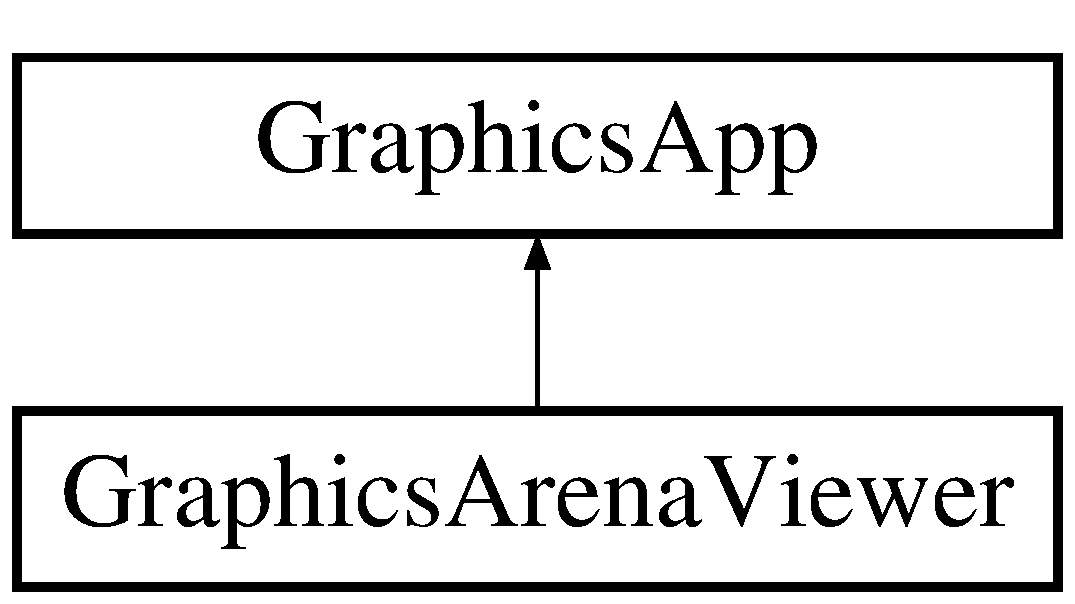
\includegraphics[height=2.000000cm]{class_graphics_arena_viewer}
\end{center}
\end{figure}
\subsection*{Public Member Functions}
\begin{DoxyCompactItemize}
\item 
\mbox{\hyperlink{class_graphics_arena_viewer_a869510833897508300da65b1eb0c5d09}{Graphics\+Arena\+Viewer}} (const struct \mbox{\hyperlink{structarena__params}{arena\+\_\+params}} $\ast$const params, \mbox{\hyperlink{class_arena}{Arena}} $\ast$arena, \mbox{\hyperlink{class_controller}{Controller}} $\ast$controller)
\begin{DoxyCompactList}\small\item\em Constructor. \end{DoxyCompactList}\item 
\mbox{\hyperlink{class_graphics_arena_viewer_a88cea02aab1550a7f315fbf4f3868109}{$\sim$\+Graphics\+Arena\+Viewer}} () override
\begin{DoxyCompactList}\small\item\em Destructor. \end{DoxyCompactList}\item 
void \mbox{\hyperlink{class_graphics_arena_viewer_aeec66666382aa0312574d70aa58de250}{Update\+Simulation}} (double dt) override
\begin{DoxyCompactList}\small\item\em Informs the \mbox{\hyperlink{class_arena}{Arena}} of the new time, so that it can update. \end{DoxyCompactList}\item 
void \mbox{\hyperlink{class_graphics_arena_viewer_a7cc65fd0e2e8c1f6138608e398c7c887}{On\+Playing\+Btn\+Pressed}} ()
\begin{DoxyCompactList}\small\item\em Handle the user pressing the pause button on the G\+UI. \end{DoxyCompactList}\item 
void \mbox{\hyperlink{class_graphics_arena_viewer_a7a573f7f55d54fd066d3d47df7a6454b}{On\+New\+Game\+Btn\+Pressed}} ()
\begin{DoxyCompactList}\small\item\em Handle the user pressing the New Game button on the G\+UI. \end{DoxyCompactList}\item 
void \mbox{\hyperlink{class_graphics_arena_viewer_a74b5c524369a62ba419c89677c646d9e}{On\+Mouse\+Move}} (\mbox{\hyperlink{common_8h_a2e3484535ee610c8e19e9859563abe48}{\+\_\+\+\_\+unused}} const Point2 \&pos, \mbox{\hyperlink{common_8h_a2e3484535ee610c8e19e9859563abe48}{\+\_\+\+\_\+unused}} const Vector2 \&delta) override
\begin{DoxyCompactList}\small\item\em Called each time the mouse moves on the screen within the G\+UI window. \end{DoxyCompactList}\item 
void \mbox{\hyperlink{class_graphics_arena_viewer_adf2fb01c3ca8b1774f031d68616b288c}{On\+Left\+Mouse\+Down}} (\mbox{\hyperlink{common_8h_a2e3484535ee610c8e19e9859563abe48}{\+\_\+\+\_\+unused}} const Point2 \&pos) override
\begin{DoxyCompactList}\small\item\em Called each time the left mouse button is clicked. \end{DoxyCompactList}\item 
void \mbox{\hyperlink{class_graphics_arena_viewer_abe4f11ab9bfb6055280ddf2b671d7032}{On\+Left\+Mouse\+Up}} (\mbox{\hyperlink{common_8h_a2e3484535ee610c8e19e9859563abe48}{\+\_\+\+\_\+unused}} const Point2 \&pos) override
\begin{DoxyCompactList}\small\item\em Called each time the left mouse button is released. \end{DoxyCompactList}\item 
void \mbox{\hyperlink{class_graphics_arena_viewer_a178a9f09ff241d4dc032b6d0998cc9c6}{On\+Right\+Mouse\+Down}} (\mbox{\hyperlink{common_8h_a2e3484535ee610c8e19e9859563abe48}{\+\_\+\+\_\+unused}} const Point2 \&pos) override
\begin{DoxyCompactList}\small\item\em Called each time the right mouse button is clicked. \end{DoxyCompactList}\item 
void \mbox{\hyperlink{class_graphics_arena_viewer_a5dfa16dca83575e253b6d3ea344f8746}{On\+Right\+Mouse\+Up}} (\mbox{\hyperlink{common_8h_a2e3484535ee610c8e19e9859563abe48}{\+\_\+\+\_\+unused}} const Point2 \&pos) override
\begin{DoxyCompactList}\small\item\em Called each time the right mouse button is released. \end{DoxyCompactList}\item 
void \mbox{\hyperlink{class_graphics_arena_viewer_ab0001d4a3ebde2b1f5b4cb7770824726}{On\+Key\+Down}} (\mbox{\hyperlink{common_8h_a2e3484535ee610c8e19e9859563abe48}{\+\_\+\+\_\+unused}} const char $\ast$c, \mbox{\hyperlink{common_8h_a2e3484535ee610c8e19e9859563abe48}{\+\_\+\+\_\+unused}} int modifiers) override
\begin{DoxyCompactList}\small\item\em Called each time a character key is pressed. \end{DoxyCompactList}\item 
void \mbox{\hyperlink{class_graphics_arena_viewer_ac3e749f6a75bdd5b32d23c9c8913f9d8}{On\+Key\+Up}} (\mbox{\hyperlink{common_8h_a2e3484535ee610c8e19e9859563abe48}{\+\_\+\+\_\+unused}} const char $\ast$c, \mbox{\hyperlink{common_8h_a2e3484535ee610c8e19e9859563abe48}{\+\_\+\+\_\+unused}} int modifiers) override
\begin{DoxyCompactList}\small\item\em Called each time a character key is released. \end{DoxyCompactList}\item 
void \mbox{\hyperlink{class_graphics_arena_viewer_a086e2e29e1a5745a8ee4f12996897b22}{On\+Special\+Key\+Up}} (\mbox{\hyperlink{common_8h_a2e3484535ee610c8e19e9859563abe48}{\+\_\+\+\_\+unused}} int key, \mbox{\hyperlink{common_8h_a2e3484535ee610c8e19e9859563abe48}{\+\_\+\+\_\+unused}} int scancode, \mbox{\hyperlink{common_8h_a2e3484535ee610c8e19e9859563abe48}{\+\_\+\+\_\+unused}} int modifiers) override
\begin{DoxyCompactList}\small\item\em Called each time a special (non-\/alphabetic) key is released. \end{DoxyCompactList}\item 
void \mbox{\hyperlink{class_graphics_arena_viewer_a7d59755e3f7674f382127fe135492eeb}{Draw\+Using\+Nano\+VG}} (N\+V\+Gcontext $\ast$ctx) override
\begin{DoxyCompactList}\small\item\em Draw the \mbox{\hyperlink{class_arena}{Arena}} with all of its entities using {\ttfamily nanogui}. \end{DoxyCompactList}\item 
\mbox{\Hypertarget{class_graphics_arena_viewer_af894508bfa039199c6ff7f1b5a7da158}\label{class_graphics_arena_viewer_af894508bfa039199c6ff7f1b5a7da158}} 
void \mbox{\hyperlink{class_graphics_arena_viewer_af894508bfa039199c6ff7f1b5a7da158}{Draw\+Using\+Open\+GL}} () override
\begin{DoxyCompactList}\small\item\em Draw using {\ttfamily Open\+GL}. This method is unimplemented, as currently we are doing all drawing with {\ttfamily nanovg} in this application, so it is empty. \end{DoxyCompactList}\item 
\mbox{\Hypertarget{class_graphics_arena_viewer_a289278f7b338fc60f983827d21b159ff}\label{class_graphics_arena_viewer_a289278f7b338fc60f983827d21b159ff}} 
\mbox{\hyperlink{class_graphics_arena_viewer}{Graphics\+Arena\+Viewer}} \& \mbox{\hyperlink{class_graphics_arena_viewer_a289278f7b338fc60f983827d21b159ff}{operator=}} (const \mbox{\hyperlink{class_graphics_arena_viewer}{Graphics\+Arena\+Viewer}} \&other)=delete
\begin{DoxyCompactList}\small\item\em Under certain circumstance, the compiler requires that the assignment operator is not defined. This {\ttfamily deletes} the default assignment operator. \end{DoxyCompactList}\item 
\mbox{\Hypertarget{class_graphics_arena_viewer_afa70b72e0769db0f3f41fe37bc540621}\label{class_graphics_arena_viewer_afa70b72e0769db0f3f41fe37bc540621}} 
\mbox{\hyperlink{class_graphics_arena_viewer_afa70b72e0769db0f3f41fe37bc540621}{Graphics\+Arena\+Viewer}} (const \mbox{\hyperlink{class_graphics_arena_viewer}{Graphics\+Arena\+Viewer}} \&other)=delete
\begin{DoxyCompactList}\small\item\em Under certain circumstance, the compiler requires that the copy constructor is not defined. This {\ttfamily deletes} the default copy constructor. \end{DoxyCompactList}\end{DoxyCompactItemize}


\subsection{Detailed Description}
An application that uses the Min\+Gfx library to open up a window that includes a few buttons for controlling the simulation and can be used to draw circles and other computer graphics. 

After constructing a new \mbox{\hyperlink{class_graphics_arena_viewer}{Graphics\+Arena\+Viewer}}, call Run to start and run the application. Run will not return until the application window is closed. Example\+:


\begin{DoxyCode}
\textcolor{keywordtype}{int} main(\textcolor{keywordtype}{int} argc, \textcolor{keywordtype}{char} **argv) \{
    RobotViewer *app = \textcolor{keyword}{new} RobotViewer();
    app->Run();
    \textcolor{keywordflow}{return} 0;
\}
\end{DoxyCode}


While the window is open Update\+Simulation will be called repeatedly, once per frame. Fill this in to update your simulation or perform any other processing that should happen over time as the simulation progresses.

Fill in the {\ttfamily On$\ast$()} methods as desired to respond to user input events.

Fill in the {\ttfamily Draw$\ast$()} methods to draw graphics on the screen using either the {\ttfamily nanovg} library or raw {\ttfamily Open\+GL}. 

\subsection{Constructor \& Destructor Documentation}
\mbox{\Hypertarget{class_graphics_arena_viewer_a869510833897508300da65b1eb0c5d09}\label{class_graphics_arena_viewer_a869510833897508300da65b1eb0c5d09}} 
\index{Graphics\+Arena\+Viewer@{Graphics\+Arena\+Viewer}!Graphics\+Arena\+Viewer@{Graphics\+Arena\+Viewer}}
\index{Graphics\+Arena\+Viewer@{Graphics\+Arena\+Viewer}!Graphics\+Arena\+Viewer@{Graphics\+Arena\+Viewer}}
\subsubsection{\texorpdfstring{Graphics\+Arena\+Viewer()}{GraphicsArenaViewer()}}
{\footnotesize\ttfamily Graphics\+Arena\+Viewer\+::\+Graphics\+Arena\+Viewer (\begin{DoxyParamCaption}\item[{const struct \mbox{\hyperlink{structarena__params}{arena\+\_\+params}} $\ast$const}]{params,  }\item[{\mbox{\hyperlink{class_arena}{Arena}} $\ast$}]{arena,  }\item[{\mbox{\hyperlink{class_controller}{Controller}} $\ast$}]{controller }\end{DoxyParamCaption})\hspace{0.3cm}{\ttfamily [explicit]}}



Constructor. 


\begin{DoxyParams}{Parameters}
{\em params} & A \mbox{\hyperlink{structarena__params}{arena\+\_\+params}} passed down from \mbox{\hyperlink{main_8cc}{main.\+cc}} for the initialization of the \mbox{\hyperlink{class_arena}{Arena}} and the entities therein. \\
\hline
\end{DoxyParams}
\mbox{\Hypertarget{class_graphics_arena_viewer_a88cea02aab1550a7f315fbf4f3868109}\label{class_graphics_arena_viewer_a88cea02aab1550a7f315fbf4f3868109}} 
\index{Graphics\+Arena\+Viewer@{Graphics\+Arena\+Viewer}!````~Graphics\+Arena\+Viewer@{$\sim$\+Graphics\+Arena\+Viewer}}
\index{````~Graphics\+Arena\+Viewer@{$\sim$\+Graphics\+Arena\+Viewer}!Graphics\+Arena\+Viewer@{Graphics\+Arena\+Viewer}}
\subsubsection{\texorpdfstring{$\sim$\+Graphics\+Arena\+Viewer()}{~GraphicsArenaViewer()}}
{\footnotesize\ttfamily Graphics\+Arena\+Viewer\+::$\sim$\+Graphics\+Arena\+Viewer (\begin{DoxyParamCaption}{ }\end{DoxyParamCaption})\hspace{0.3cm}{\ttfamily [inline]}, {\ttfamily [override]}}



Destructor. 

{\ttfamily delete} the contained \mbox{\hyperlink{class_arena}{Arena}}. 

\subsection{Member Function Documentation}
\mbox{\Hypertarget{class_graphics_arena_viewer_a7d59755e3f7674f382127fe135492eeb}\label{class_graphics_arena_viewer_a7d59755e3f7674f382127fe135492eeb}} 
\index{Graphics\+Arena\+Viewer@{Graphics\+Arena\+Viewer}!Draw\+Using\+Nano\+VG@{Draw\+Using\+Nano\+VG}}
\index{Draw\+Using\+Nano\+VG@{Draw\+Using\+Nano\+VG}!Graphics\+Arena\+Viewer@{Graphics\+Arena\+Viewer}}
\subsubsection{\texorpdfstring{Draw\+Using\+Nano\+V\+G()}{DrawUsingNanoVG()}}
{\footnotesize\ttfamily void Graphics\+Arena\+Viewer\+::\+Draw\+Using\+Nano\+VG (\begin{DoxyParamCaption}\item[{N\+V\+Gcontext $\ast$}]{ctx }\end{DoxyParamCaption})\hspace{0.3cm}{\ttfamily [override]}}



Draw the \mbox{\hyperlink{class_arena}{Arena}} with all of its entities using {\ttfamily nanogui}. 

This is the primary driver for drawing all entities in the \mbox{\hyperlink{class_arena}{Arena}}. It is called at each iteration of {\ttfamily nanogui\+::mainloop()}.


\begin{DoxyParams}[1]{Parameters}
\mbox{\tt in}  & {\em ctx} & Context for nanogui. \\
\hline
\end{DoxyParams}
\mbox{\Hypertarget{class_graphics_arena_viewer_ab0001d4a3ebde2b1f5b4cb7770824726}\label{class_graphics_arena_viewer_ab0001d4a3ebde2b1f5b4cb7770824726}} 
\index{Graphics\+Arena\+Viewer@{Graphics\+Arena\+Viewer}!On\+Key\+Down@{On\+Key\+Down}}
\index{On\+Key\+Down@{On\+Key\+Down}!Graphics\+Arena\+Viewer@{Graphics\+Arena\+Viewer}}
\subsubsection{\texorpdfstring{On\+Key\+Down()}{OnKeyDown()}}
{\footnotesize\ttfamily void Graphics\+Arena\+Viewer\+::\+On\+Key\+Down (\begin{DoxyParamCaption}\item[{\mbox{\hyperlink{common_8h_a2e3484535ee610c8e19e9859563abe48}{\+\_\+\+\_\+unused}} const char $\ast$}]{c,  }\item[{\mbox{\hyperlink{common_8h_a2e3484535ee610c8e19e9859563abe48}{\+\_\+\+\_\+unused}} int}]{modifiers }\end{DoxyParamCaption})\hspace{0.3cm}{\ttfamily [inline]}, {\ttfamily [override]}}



Called each time a character key is pressed. 


\begin{DoxyParams}[1]{Parameters}
\mbox{\tt in}  & {\em c} & Character representing a key that was pressed. \\
\hline
\mbox{\tt in}  & {\em modifiers} & Any modifier keys that were also pressed. \\
\hline
\end{DoxyParams}
\mbox{\Hypertarget{class_graphics_arena_viewer_ac3e749f6a75bdd5b32d23c9c8913f9d8}\label{class_graphics_arena_viewer_ac3e749f6a75bdd5b32d23c9c8913f9d8}} 
\index{Graphics\+Arena\+Viewer@{Graphics\+Arena\+Viewer}!On\+Key\+Up@{On\+Key\+Up}}
\index{On\+Key\+Up@{On\+Key\+Up}!Graphics\+Arena\+Viewer@{Graphics\+Arena\+Viewer}}
\subsubsection{\texorpdfstring{On\+Key\+Up()}{OnKeyUp()}}
{\footnotesize\ttfamily void Graphics\+Arena\+Viewer\+::\+On\+Key\+Up (\begin{DoxyParamCaption}\item[{\mbox{\hyperlink{common_8h_a2e3484535ee610c8e19e9859563abe48}{\+\_\+\+\_\+unused}} const char $\ast$}]{c,  }\item[{\mbox{\hyperlink{common_8h_a2e3484535ee610c8e19e9859563abe48}{\+\_\+\+\_\+unused}} int}]{modifiers }\end{DoxyParamCaption})\hspace{0.3cm}{\ttfamily [inline]}, {\ttfamily [override]}}



Called each time a character key is released. 


\begin{DoxyParams}[1]{Parameters}
\mbox{\tt in}  & {\em c} & Character representing a key that was released. \\
\hline
\mbox{\tt in}  & {\em modifiers} & Any modifier keys that were held with the key. \\
\hline
\end{DoxyParams}
\mbox{\Hypertarget{class_graphics_arena_viewer_adf2fb01c3ca8b1774f031d68616b288c}\label{class_graphics_arena_viewer_adf2fb01c3ca8b1774f031d68616b288c}} 
\index{Graphics\+Arena\+Viewer@{Graphics\+Arena\+Viewer}!On\+Left\+Mouse\+Down@{On\+Left\+Mouse\+Down}}
\index{On\+Left\+Mouse\+Down@{On\+Left\+Mouse\+Down}!Graphics\+Arena\+Viewer@{Graphics\+Arena\+Viewer}}
\subsubsection{\texorpdfstring{On\+Left\+Mouse\+Down()}{OnLeftMouseDown()}}
{\footnotesize\ttfamily void Graphics\+Arena\+Viewer\+::\+On\+Left\+Mouse\+Down (\begin{DoxyParamCaption}\item[{\mbox{\hyperlink{common_8h_a2e3484535ee610c8e19e9859563abe48}{\+\_\+\+\_\+unused}} const Point2 \&}]{pos }\end{DoxyParamCaption})\hspace{0.3cm}{\ttfamily [inline]}, {\ttfamily [override]}}



Called each time the left mouse button is clicked. 

Origin is at the lower left of the window. This function is a stub.


\begin{DoxyParams}[1]{Parameters}
\mbox{\tt in}  & {\em pos} & The position of the release. \\
\hline
\end{DoxyParams}
\mbox{\Hypertarget{class_graphics_arena_viewer_abe4f11ab9bfb6055280ddf2b671d7032}\label{class_graphics_arena_viewer_abe4f11ab9bfb6055280ddf2b671d7032}} 
\index{Graphics\+Arena\+Viewer@{Graphics\+Arena\+Viewer}!On\+Left\+Mouse\+Up@{On\+Left\+Mouse\+Up}}
\index{On\+Left\+Mouse\+Up@{On\+Left\+Mouse\+Up}!Graphics\+Arena\+Viewer@{Graphics\+Arena\+Viewer}}
\subsubsection{\texorpdfstring{On\+Left\+Mouse\+Up()}{OnLeftMouseUp()}}
{\footnotesize\ttfamily void Graphics\+Arena\+Viewer\+::\+On\+Left\+Mouse\+Up (\begin{DoxyParamCaption}\item[{\mbox{\hyperlink{common_8h_a2e3484535ee610c8e19e9859563abe48}{\+\_\+\+\_\+unused}} const Point2 \&}]{pos }\end{DoxyParamCaption})\hspace{0.3cm}{\ttfamily [inline]}, {\ttfamily [override]}}



Called each time the left mouse button is released. 

Origin is at the lower left of the window. This function is a stub.


\begin{DoxyParams}[1]{Parameters}
\mbox{\tt in}  & {\em pos} & The position of the release. \\
\hline
\end{DoxyParams}
\mbox{\Hypertarget{class_graphics_arena_viewer_a74b5c524369a62ba419c89677c646d9e}\label{class_graphics_arena_viewer_a74b5c524369a62ba419c89677c646d9e}} 
\index{Graphics\+Arena\+Viewer@{Graphics\+Arena\+Viewer}!On\+Mouse\+Move@{On\+Mouse\+Move}}
\index{On\+Mouse\+Move@{On\+Mouse\+Move}!Graphics\+Arena\+Viewer@{Graphics\+Arena\+Viewer}}
\subsubsection{\texorpdfstring{On\+Mouse\+Move()}{OnMouseMove()}}
{\footnotesize\ttfamily void Graphics\+Arena\+Viewer\+::\+On\+Mouse\+Move (\begin{DoxyParamCaption}\item[{\mbox{\hyperlink{common_8h_a2e3484535ee610c8e19e9859563abe48}{\+\_\+\+\_\+unused}} const Point2 \&}]{pos,  }\item[{\mbox{\hyperlink{common_8h_a2e3484535ee610c8e19e9859563abe48}{\+\_\+\+\_\+unused}} const Vector2 \&}]{delta }\end{DoxyParamCaption})\hspace{0.3cm}{\ttfamily [inline]}, {\ttfamily [override]}}



Called each time the mouse moves on the screen within the G\+UI window. 

Origin is at the lower left of the window. This function is a stub.


\begin{DoxyParams}[1]{Parameters}
\mbox{\tt in}  & {\em pos} & The position of the release. \\
\hline
\mbox{\tt in}  & {\em delta} & How far the mouse has moved. \\
\hline
\end{DoxyParams}
\mbox{\Hypertarget{class_graphics_arena_viewer_a7a573f7f55d54fd066d3d47df7a6454b}\label{class_graphics_arena_viewer_a7a573f7f55d54fd066d3d47df7a6454b}} 
\index{Graphics\+Arena\+Viewer@{Graphics\+Arena\+Viewer}!On\+New\+Game\+Btn\+Pressed@{On\+New\+Game\+Btn\+Pressed}}
\index{On\+New\+Game\+Btn\+Pressed@{On\+New\+Game\+Btn\+Pressed}!Graphics\+Arena\+Viewer@{Graphics\+Arena\+Viewer}}
\subsubsection{\texorpdfstring{On\+New\+Game\+Btn\+Pressed()}{OnNewGameBtnPressed()}}
{\footnotesize\ttfamily void Graphics\+Arena\+Viewer\+::\+On\+New\+Game\+Btn\+Pressed (\begin{DoxyParamCaption}{ }\end{DoxyParamCaption})}



Handle the user pressing the New Game button on the G\+UI. 

This will reset the game to a new state. \mbox{\Hypertarget{class_graphics_arena_viewer_a7cc65fd0e2e8c1f6138608e398c7c887}\label{class_graphics_arena_viewer_a7cc65fd0e2e8c1f6138608e398c7c887}} 
\index{Graphics\+Arena\+Viewer@{Graphics\+Arena\+Viewer}!On\+Playing\+Btn\+Pressed@{On\+Playing\+Btn\+Pressed}}
\index{On\+Playing\+Btn\+Pressed@{On\+Playing\+Btn\+Pressed}!Graphics\+Arena\+Viewer@{Graphics\+Arena\+Viewer}}
\subsubsection{\texorpdfstring{On\+Playing\+Btn\+Pressed()}{OnPlayingBtnPressed()}}
{\footnotesize\ttfamily void Graphics\+Arena\+Viewer\+::\+On\+Playing\+Btn\+Pressed (\begin{DoxyParamCaption}{ }\end{DoxyParamCaption})}



Handle the user pressing the pause button on the G\+UI. 

This will freeze the graphics--no update, until the pause button is pressed again. \mbox{\Hypertarget{class_graphics_arena_viewer_a178a9f09ff241d4dc032b6d0998cc9c6}\label{class_graphics_arena_viewer_a178a9f09ff241d4dc032b6d0998cc9c6}} 
\index{Graphics\+Arena\+Viewer@{Graphics\+Arena\+Viewer}!On\+Right\+Mouse\+Down@{On\+Right\+Mouse\+Down}}
\index{On\+Right\+Mouse\+Down@{On\+Right\+Mouse\+Down}!Graphics\+Arena\+Viewer@{Graphics\+Arena\+Viewer}}
\subsubsection{\texorpdfstring{On\+Right\+Mouse\+Down()}{OnRightMouseDown()}}
{\footnotesize\ttfamily void Graphics\+Arena\+Viewer\+::\+On\+Right\+Mouse\+Down (\begin{DoxyParamCaption}\item[{\mbox{\hyperlink{common_8h_a2e3484535ee610c8e19e9859563abe48}{\+\_\+\+\_\+unused}} const Point2 \&}]{pos }\end{DoxyParamCaption})\hspace{0.3cm}{\ttfamily [inline]}, {\ttfamily [override]}}



Called each time the right mouse button is clicked. 

Origin is at the lower left of the window. This function is a stub.


\begin{DoxyParams}[1]{Parameters}
\mbox{\tt in}  & {\em pos} & The position of the release. \\
\hline
\end{DoxyParams}
\mbox{\Hypertarget{class_graphics_arena_viewer_a5dfa16dca83575e253b6d3ea344f8746}\label{class_graphics_arena_viewer_a5dfa16dca83575e253b6d3ea344f8746}} 
\index{Graphics\+Arena\+Viewer@{Graphics\+Arena\+Viewer}!On\+Right\+Mouse\+Up@{On\+Right\+Mouse\+Up}}
\index{On\+Right\+Mouse\+Up@{On\+Right\+Mouse\+Up}!Graphics\+Arena\+Viewer@{Graphics\+Arena\+Viewer}}
\subsubsection{\texorpdfstring{On\+Right\+Mouse\+Up()}{OnRightMouseUp()}}
{\footnotesize\ttfamily void Graphics\+Arena\+Viewer\+::\+On\+Right\+Mouse\+Up (\begin{DoxyParamCaption}\item[{\mbox{\hyperlink{common_8h_a2e3484535ee610c8e19e9859563abe48}{\+\_\+\+\_\+unused}} const Point2 \&}]{pos }\end{DoxyParamCaption})\hspace{0.3cm}{\ttfamily [inline]}, {\ttfamily [override]}}



Called each time the right mouse button is released. 

Origin is at the lower left of the window. This function is a stub.


\begin{DoxyParams}[1]{Parameters}
\mbox{\tt in}  & {\em pos} & The position of the release. \\
\hline
\end{DoxyParams}
\mbox{\Hypertarget{class_graphics_arena_viewer_a086e2e29e1a5745a8ee4f12996897b22}\label{class_graphics_arena_viewer_a086e2e29e1a5745a8ee4f12996897b22}} 
\index{Graphics\+Arena\+Viewer@{Graphics\+Arena\+Viewer}!On\+Special\+Key\+Up@{On\+Special\+Key\+Up}}
\index{On\+Special\+Key\+Up@{On\+Special\+Key\+Up}!Graphics\+Arena\+Viewer@{Graphics\+Arena\+Viewer}}
\subsubsection{\texorpdfstring{On\+Special\+Key\+Up()}{OnSpecialKeyUp()}}
{\footnotesize\ttfamily void Graphics\+Arena\+Viewer\+::\+On\+Special\+Key\+Up (\begin{DoxyParamCaption}\item[{\mbox{\hyperlink{common_8h_a2e3484535ee610c8e19e9859563abe48}{\+\_\+\+\_\+unused}} int}]{key,  }\item[{\mbox{\hyperlink{common_8h_a2e3484535ee610c8e19e9859563abe48}{\+\_\+\+\_\+unused}} int}]{scancode,  }\item[{\mbox{\hyperlink{common_8h_a2e3484535ee610c8e19e9859563abe48}{\+\_\+\+\_\+unused}} int}]{modifiers }\end{DoxyParamCaption})\hspace{0.3cm}{\ttfamily [inline]}, {\ttfamily [override]}}



Called each time a special (non-\/alphabetic) key is released. 


\begin{DoxyParams}[1]{Parameters}
\mbox{\tt in}  & {\em key} & The key that was released. \\
\hline
\mbox{\tt in}  & {\em scancode} & The scancode corresponding to the key. \\
\hline
\mbox{\tt in}  & {\em modifiers} & Any modifier keys that were also pressed. \\
\hline
\end{DoxyParams}
\mbox{\Hypertarget{class_graphics_arena_viewer_aeec66666382aa0312574d70aa58de250}\label{class_graphics_arena_viewer_aeec66666382aa0312574d70aa58de250}} 
\index{Graphics\+Arena\+Viewer@{Graphics\+Arena\+Viewer}!Update\+Simulation@{Update\+Simulation}}
\index{Update\+Simulation@{Update\+Simulation}!Graphics\+Arena\+Viewer@{Graphics\+Arena\+Viewer}}
\subsubsection{\texorpdfstring{Update\+Simulation()}{UpdateSimulation()}}
{\footnotesize\ttfamily void Graphics\+Arena\+Viewer\+::\+Update\+Simulation (\begin{DoxyParamCaption}\item[{double}]{dt }\end{DoxyParamCaption})\hspace{0.3cm}{\ttfamily [override]}}



Informs the \mbox{\hyperlink{class_arena}{Arena}} of the new time, so that it can update. 


\begin{DoxyParams}{Parameters}
{\em dt} & The new timestep. \\
\hline
\end{DoxyParams}


The documentation for this class was generated from the following files\+:\begin{DoxyCompactItemize}
\item 
src/\mbox{\hyperlink{graphics__arena__viewer_8h}{graphics\+\_\+arena\+\_\+viewer.\+h}}\item 
src/\mbox{\hyperlink{graphics__arena__viewer_8cc}{graphics\+\_\+arena\+\_\+viewer.\+cc}}\end{DoxyCompactItemize}

\hypertarget{class_light}{}\section{Light Class Reference}
\label{class_light}\index{Light@{Light}}


Class representing a mobile light within the \mbox{\hyperlink{class_arena}{Arena}}.  




{\ttfamily \#include $<$light.\+h$>$}

Inheritance diagram for Light\+:\begin{figure}[H]
\begin{center}
\leavevmode
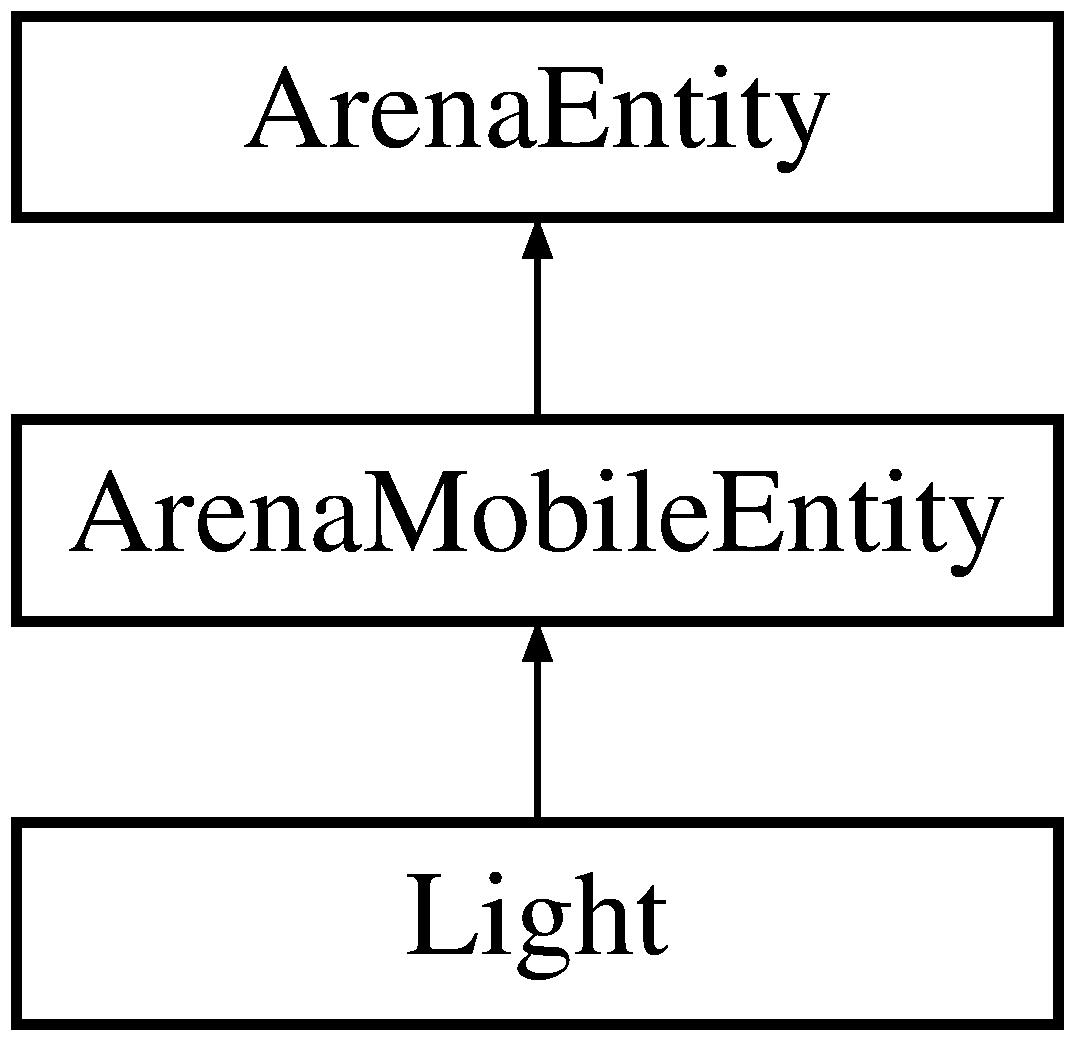
\includegraphics[height=3.000000cm]{class_light}
\end{center}
\end{figure}
\subsection*{Public Member Functions}
\begin{DoxyCompactItemize}
\item 
\mbox{\Hypertarget{class_light_aeb5df09a25a32f19fdffa761268ba24f}\label{class_light_aeb5df09a25a32f19fdffa761268ba24f}} 
\mbox{\hyperlink{class_light_aeb5df09a25a32f19fdffa761268ba24f}{Light}} ()
\begin{DoxyCompactList}\small\item\em Constructor. \end{DoxyCompactList}\item 
\mbox{\Hypertarget{class_light_a49b2e32cf8173353ac4689fdadbb95d5}\label{class_light_a49b2e32cf8173353ac4689fdadbb95d5}} 
std\+::string \mbox{\hyperlink{class_light_a49b2e32cf8173353ac4689fdadbb95d5}{get\+\_\+name}} () const override
\begin{DoxyCompactList}\small\item\em Get the name of the \mbox{\hyperlink{class_light}{Light}} for visualization purposes, and to aid in debugging. \end{DoxyCompactList}\item 
\mbox{\Hypertarget{class_light_a61485eb0684868b503e1b96e6a3206c3}\label{class_light_a61485eb0684868b503e1b96e6a3206c3}} 
void \mbox{\hyperlink{class_light_a61485eb0684868b503e1b96e6a3206c3}{Reset}} () override
\begin{DoxyCompactList}\small\item\em Reset the \mbox{\hyperlink{class_robot}{Robot}} to a newly constructed state (needed for reset button to work in G\+UI). \end{DoxyCompactList}\item 
void \mbox{\hyperlink{class_light_a97934eec7489f9b072534f5e30a2d90d}{Timestep\+Update}} (unsigned int dt) override
\begin{DoxyCompactList}\small\item\em Update the light\textquotesingle{}s position after the specified duration has passed. \end{DoxyCompactList}\item 
\mbox{\Hypertarget{class_light_a7b8ef784bba9ec5725b0b0595e7da850}\label{class_light_a7b8ef784bba9ec5725b0b0595e7da850}} 
void \mbox{\hyperlink{class_light_a7b8ef784bba9ec5725b0b0595e7da850}{Handle\+Collision}} (Entity\+Type object\+\_\+type, \mbox{\hyperlink{class_arena_entity}{Arena\+Entity}} $\ast$object=N\+U\+LL)
\begin{DoxyCompactList}\small\item\em Handles the collision by setting the sensor to activated. \end{DoxyCompactList}\item 
\mbox{\Hypertarget{class_light_ac4b1010649835f0572e5215a8b58d76d}\label{class_light_ac4b1010649835f0572e5215a8b58d76d}} 
void \mbox{\hyperlink{class_light_ac4b1010649835f0572e5215a8b58d76d}{reset\+\_\+arc\+\_\+time}} ()
\begin{DoxyCompactList}\small\item\em Resets the arc time to the maximum. \end{DoxyCompactList}\end{DoxyCompactItemize}
\subsection*{Additional Inherited Members}


\subsection{Detailed Description}
Class representing a mobile light within the \mbox{\hyperlink{class_arena}{Arena}}. 

The lights have a wheel velocity which controls their movement. With that they also have Timestep\+Update which controls the visual movement. Handle\+Collision controls what the light does when it collides with an entity. 

\subsection{Member Function Documentation}
\mbox{\Hypertarget{class_light_a97934eec7489f9b072534f5e30a2d90d}\label{class_light_a97934eec7489f9b072534f5e30a2d90d}} 
\index{Light@{Light}!Timestep\+Update@{Timestep\+Update}}
\index{Timestep\+Update@{Timestep\+Update}!Light@{Light}}
\subsubsection{\texorpdfstring{Timestep\+Update()}{TimestepUpdate()}}
{\footnotesize\ttfamily void Light\+::\+Timestep\+Update (\begin{DoxyParamCaption}\item[{unsigned int}]{dt }\end{DoxyParamCaption})\hspace{0.3cm}{\ttfamily [override]}}



Update the light\textquotesingle{}s position after the specified duration has passed. 


\begin{DoxyParams}{Parameters}
{\em dt} & The \# of timesteps that have elapsed since the last update. \\
\hline
\end{DoxyParams}


The documentation for this class was generated from the following files\+:\begin{DoxyCompactItemize}
\item 
src/\mbox{\hyperlink{light_8h}{light.\+h}}\item 
src/\mbox{\hyperlink{light_8cc}{light.\+cc}}\end{DoxyCompactItemize}

\hypertarget{class_light_sensor}{}\section{Light\+Sensor Class Reference}
\label{class_light_sensor}\index{Light\+Sensor@{Light\+Sensor}}


Class representing a light sensor for the robot.  




{\ttfamily \#include $<$light\+\_\+sensor.\+h$>$}

Inheritance diagram for Light\+Sensor\+:\begin{figure}[H]
\begin{center}
\leavevmode
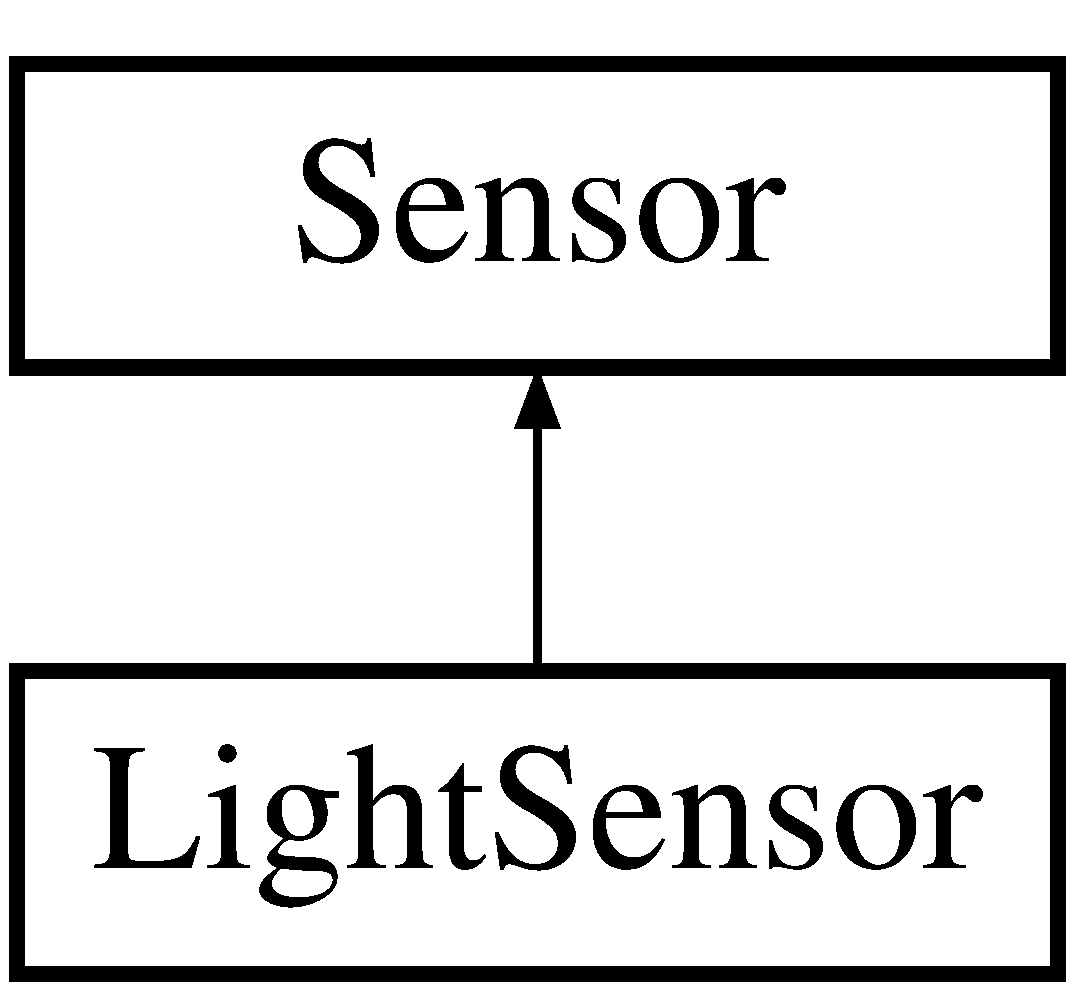
\includegraphics[height=2.000000cm]{class_light_sensor}
\end{center}
\end{figure}
\subsection*{Public Member Functions}
\begin{DoxyCompactItemize}
\item 
\mbox{\hyperlink{class_light_sensor_ab2d2e9a3c5051d283eeee95dca6c582f}{Light\+Sensor}} (\mbox{\hyperlink{class_robot}{Robot}} $\ast$robot, double sensor\+\_\+angle)
\begin{DoxyCompactList}\small\item\em Constructor. \end{DoxyCompactList}\item 
\mbox{\Hypertarget{class_light_sensor_a1d226e9f15af1b7245f7a2a057f8ea9c}\label{class_light_sensor_a1d226e9f15af1b7245f7a2a057f8ea9c}} 
\mbox{\hyperlink{class_light_sensor_a1d226e9f15af1b7245f7a2a057f8ea9c}{$\sim$\+Light\+Sensor}} ()=default
\begin{DoxyCompactList}\small\item\em Default destructor. \end{DoxyCompactList}\item 
void \mbox{\hyperlink{class_light_sensor_ad03aaaf3b16b583ca5b5851d9887d078}{Notify}} (\mbox{\hyperlink{struct_pose}{Pose}} entity\+\_\+pose) override
\begin{DoxyCompactList}\small\item\em Gives a sensor reading based upon the position passed in. \end{DoxyCompactList}\item 
\mbox{\Hypertarget{class_light_sensor_a8b8643f10dc619dd8f31ab87034a04f6}\label{class_light_sensor_a8b8643f10dc619dd8f31ab87034a04f6}} 
void \mbox{\hyperlink{class_light_sensor_a8b8643f10dc619dd8f31ab87034a04f6}{Reset}} () override
\begin{DoxyCompactList}\small\item\em Resets the position and the sensor reading. \end{DoxyCompactList}\end{DoxyCompactItemize}
\subsection*{Additional Inherited Members}


\subsection{Detailed Description}
Class representing a light sensor for the robot. 

Light\+Sensors are what detect the proximity of the robot to the light. They make sure the robot follows its behavior

The Light\+Sensors get notified by light and create readings based upon their proximity to the light. 

\subsection{Constructor \& Destructor Documentation}
\mbox{\Hypertarget{class_light_sensor_ab2d2e9a3c5051d283eeee95dca6c582f}\label{class_light_sensor_ab2d2e9a3c5051d283eeee95dca6c582f}} 
\index{Light\+Sensor@{Light\+Sensor}!Light\+Sensor@{Light\+Sensor}}
\index{Light\+Sensor@{Light\+Sensor}!Light\+Sensor@{Light\+Sensor}}
\subsubsection{\texorpdfstring{Light\+Sensor()}{LightSensor()}}
{\footnotesize\ttfamily Light\+Sensor\+::\+Light\+Sensor (\begin{DoxyParamCaption}\item[{\mbox{\hyperlink{class_robot}{Robot}} $\ast$}]{robot,  }\item[{double}]{sensor\+\_\+angle }\end{DoxyParamCaption})}



Constructor. 


\begin{DoxyParams}[1]{Parameters}
\mbox{\tt in}  & {\em robot} & -\/ reference to the robot of this sensor \\
\hline
\mbox{\tt in}  & {\em sensor\+\_\+angle} & -\/ the location of the sensor \\
\hline
\end{DoxyParams}


\subsection{Member Function Documentation}
\mbox{\Hypertarget{class_light_sensor_ad03aaaf3b16b583ca5b5851d9887d078}\label{class_light_sensor_ad03aaaf3b16b583ca5b5851d9887d078}} 
\index{Light\+Sensor@{Light\+Sensor}!Notify@{Notify}}
\index{Notify@{Notify}!Light\+Sensor@{Light\+Sensor}}
\subsubsection{\texorpdfstring{Notify()}{Notify()}}
{\footnotesize\ttfamily void Light\+Sensor\+::\+Notify (\begin{DoxyParamCaption}\item[{\mbox{\hyperlink{struct_pose}{Pose}}}]{entity\+\_\+pose }\end{DoxyParamCaption})\hspace{0.3cm}{\ttfamily [override]}}



Gives a sensor reading based upon the position passed in. 


\begin{DoxyParams}{Parameters}
{\em entity\+\_\+pose} & -\/ the entity to base the reading off of \\
\hline
\end{DoxyParams}


The documentation for this class was generated from the following files\+:\begin{DoxyCompactItemize}
\item 
src/\mbox{\hyperlink{light__sensor_8h}{light\+\_\+sensor.\+h}}\item 
src/light\+\_\+sensor.\+cc\end{DoxyCompactItemize}

\hypertarget{class_motion_behavior}{}\section{Motion\+Behavior Class Reference}
\label{class_motion_behavior}\index{Motion\+Behavior@{Motion\+Behavior}}


Class managing an \mbox{\hyperlink{class_arena_mobile_entity}{Arena\+Mobile\+Entity}}\textquotesingle{}s position.  




{\ttfamily \#include $<$motion\+\_\+behavior.\+h$>$}

Inheritance diagram for Motion\+Behavior\+:\begin{figure}[H]
\begin{center}
\leavevmode
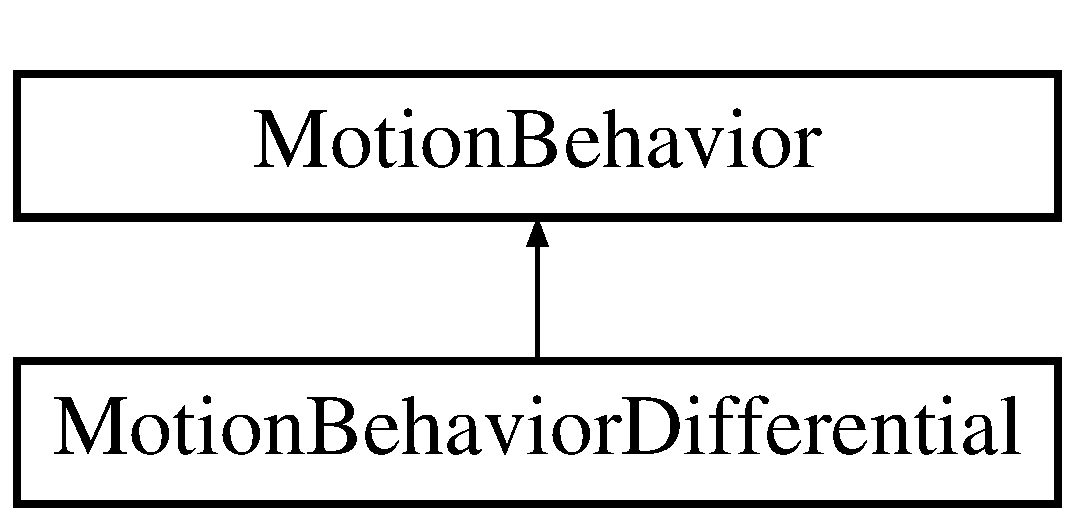
\includegraphics[height=2.000000cm]{class_motion_behavior}
\end{center}
\end{figure}
\subsection*{Public Member Functions}
\begin{DoxyCompactItemize}
\item 
\mbox{\Hypertarget{class_motion_behavior_aa2d5f7d563f4fdb5702edb8367eaa6e7}\label{class_motion_behavior_aa2d5f7d563f4fdb5702edb8367eaa6e7}} 
\mbox{\hyperlink{class_motion_behavior_aa2d5f7d563f4fdb5702edb8367eaa6e7}{Motion\+Behavior}} (\mbox{\hyperlink{class_arena_mobile_entity}{Arena\+Mobile\+Entity}} $\ast$ent)
\begin{DoxyCompactList}\small\item\em Explicit value constructor. \end{DoxyCompactList}\item 
\mbox{\Hypertarget{class_motion_behavior_a55f036f1b5c0b776656ebda7bad7ff17}\label{class_motion_behavior_a55f036f1b5c0b776656ebda7bad7ff17}} 
virtual \mbox{\hyperlink{class_motion_behavior_a55f036f1b5c0b776656ebda7bad7ff17}{$\sim$\+Motion\+Behavior}} ()=default
\begin{DoxyCompactList}\small\item\em Default destructor. \end{DoxyCompactList}\item 
\mbox{\Hypertarget{class_motion_behavior_a5fe8e8a49e8cb34519a34ca652a23143}\label{class_motion_behavior_a5fe8e8a49e8cb34519a34ca652a23143}} 
\mbox{\hyperlink{class_motion_behavior_a5fe8e8a49e8cb34519a34ca652a23143}{Motion\+Behavior}} (const \mbox{\hyperlink{class_motion_behavior}{Motion\+Behavior}} \&other)=default
\begin{DoxyCompactList}\small\item\em Default copy constructor. \end{DoxyCompactList}\item 
\mbox{\Hypertarget{class_motion_behavior_a227057c1862c64bbc609705205473abc}\label{class_motion_behavior_a227057c1862c64bbc609705205473abc}} 
\mbox{\hyperlink{class_motion_behavior}{Motion\+Behavior}} \& \mbox{\hyperlink{class_motion_behavior_a227057c1862c64bbc609705205473abc}{operator=}} (const \mbox{\hyperlink{class_motion_behavior}{Motion\+Behavior}} \&other)=default
\begin{DoxyCompactList}\small\item\em Default assignment operator overload. \end{DoxyCompactList}\item 
virtual void \mbox{\hyperlink{class_motion_behavior_a804f440bb7f03f19abec79a1ab671494}{Update\+Pose}} (double dt, \mbox{\hyperlink{struct_wheel_velocity}{Wheel\+Velocity}} vel=\mbox{\hyperlink{struct_wheel_velocity}{Wheel\+Velocity}}())
\begin{DoxyCompactList}\small\item\em Update the position (and possibly orientation) for an \mbox{\hyperlink{class_arena_mobile_entity}{Arena\+Mobile\+Entity}}, foodd on its current position and velocity. \end{DoxyCompactList}\item 
\mbox{\Hypertarget{class_motion_behavior_a1daf82b16d312ba6f5f71178e7fafa79}\label{class_motion_behavior_a1daf82b16d312ba6f5f71178e7fafa79}} 
\mbox{\hyperlink{class_arena_mobile_entity}{Arena\+Mobile\+Entity}} $\ast$ \mbox{\hyperlink{class_motion_behavior_a1daf82b16d312ba6f5f71178e7fafa79}{get\+\_\+entity}} ()
\begin{DoxyCompactList}\small\item\em Getter of entity in which this class was created. \end{DoxyCompactList}\end{DoxyCompactItemize}
\subsection*{Protected Attributes}
\begin{DoxyCompactItemize}
\item 
\mbox{\Hypertarget{class_motion_behavior_a9254cf197657a2a52d89dbc01da31b8f}\label{class_motion_behavior_a9254cf197657a2a52d89dbc01da31b8f}} 
\mbox{\hyperlink{class_arena_mobile_entity}{Arena\+Mobile\+Entity}} $\ast$ {\bfseries entity\+\_\+}
\end{DoxyCompactItemize}


\subsection{Detailed Description}
Class managing an \mbox{\hyperlink{class_arena_mobile_entity}{Arena\+Mobile\+Entity}}\textquotesingle{}s position. 

Update the position foodd on the current speed and position. This is simple, but the framework allows for more sophisticated models of motion in which each wheel has different speeds. 

\subsection{Member Function Documentation}
\mbox{\Hypertarget{class_motion_behavior_a804f440bb7f03f19abec79a1ab671494}\label{class_motion_behavior_a804f440bb7f03f19abec79a1ab671494}} 
\index{Motion\+Behavior@{Motion\+Behavior}!Update\+Pose@{Update\+Pose}}
\index{Update\+Pose@{Update\+Pose}!Motion\+Behavior@{Motion\+Behavior}}
\subsubsection{\texorpdfstring{Update\+Pose()}{UpdatePose()}}
{\footnotesize\ttfamily void Motion\+Behavior\+::\+Update\+Pose (\begin{DoxyParamCaption}\item[{double}]{dt,  }\item[{\mbox{\hyperlink{struct_wheel_velocity}{Wheel\+Velocity}}}]{vel = {\ttfamily \mbox{\hyperlink{struct_wheel_velocity}{Wheel\+Velocity}}()} }\end{DoxyParamCaption})\hspace{0.3cm}{\ttfamily [virtual]}}



Update the position (and possibly orientation) for an \mbox{\hyperlink{class_arena_mobile_entity}{Arena\+Mobile\+Entity}}, foodd on its current position and velocity. 


\begin{DoxyParams}[1]{Parameters}
\mbox{\tt in}  & {\em dt} & \# of timesteps elapsed since the last update. \\
\hline
\mbox{\tt in}  & {\em vel} & \mbox{\hyperlink{struct_wheel_velocity}{Wheel\+Velocity}} stored within the motion handler \\
\hline
\end{DoxyParams}


Reimplemented in \mbox{\hyperlink{class_motion_behavior_differential_a929c3a05aa2072acf2a508109b1259ef}{Motion\+Behavior\+Differential}}.



The documentation for this class was generated from the following files\+:\begin{DoxyCompactItemize}
\item 
src/\mbox{\hyperlink{motion__behavior_8h}{motion\+\_\+behavior.\+h}}\item 
src/\mbox{\hyperlink{motion__behavior_8cc}{motion\+\_\+behavior.\+cc}}\end{DoxyCompactItemize}

\hypertarget{class_motion_behavior_differential}{}\section{Motion\+Behavior\+Differential Class Reference}
\label{class_motion_behavior_differential}\index{Motion\+Behavior\+Differential@{Motion\+Behavior\+Differential}}


A simple model of differential drive kinematics foodd on the notes here\+: $\sim$https\+://chess.eecs.\+berkeley.\+edu/eecs149/documentation/differential\+Drive.pdf$\sim$.  




{\ttfamily \#include $<$motion\+\_\+behavior\+\_\+differential.\+h$>$}

Inheritance diagram for Motion\+Behavior\+Differential\+:\begin{figure}[H]
\begin{center}
\leavevmode
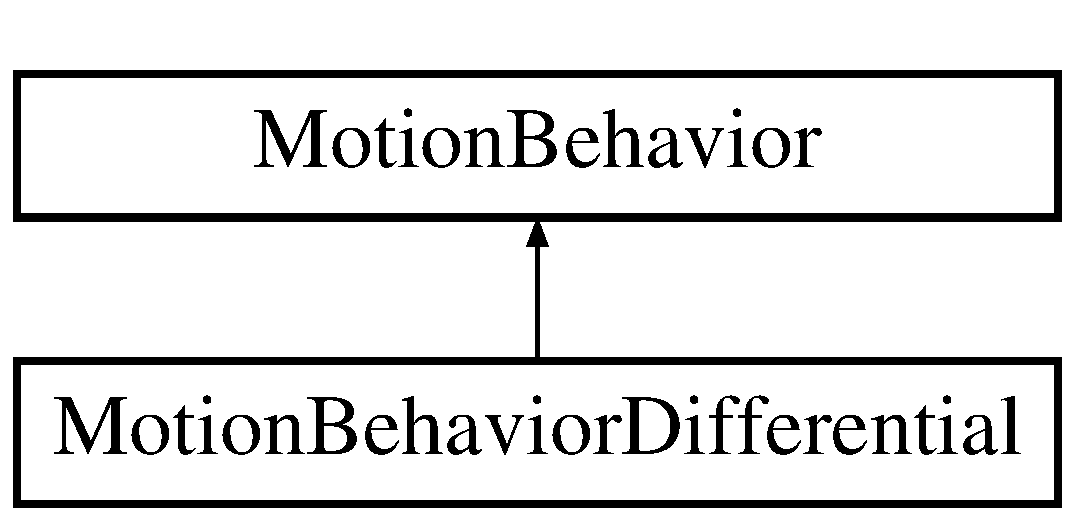
\includegraphics[height=2.000000cm]{class_motion_behavior_differential}
\end{center}
\end{figure}
\subsection*{Public Member Functions}
\begin{DoxyCompactItemize}
\item 
\mbox{\Hypertarget{class_motion_behavior_differential_a8815791ac85212945862454560279d28}\label{class_motion_behavior_differential_a8815791ac85212945862454560279d28}} 
{\bfseries Motion\+Behavior\+Differential} (\mbox{\hyperlink{class_arena_mobile_entity}{Arena\+Mobile\+Entity}} $\ast$entity)
\item 
\mbox{\Hypertarget{class_motion_behavior_differential_aeaa480aac3de205e1d177c4b4ad73ed6}\label{class_motion_behavior_differential_aeaa480aac3de205e1d177c4b4ad73ed6}} 
{\bfseries Motion\+Behavior\+Differential} (const \mbox{\hyperlink{class_motion_behavior_differential}{Motion\+Behavior\+Differential}} \&other)=default
\item 
\mbox{\Hypertarget{class_motion_behavior_differential_aaf4edbc2e349cb8cdbb033b16b1aef22}\label{class_motion_behavior_differential_aaf4edbc2e349cb8cdbb033b16b1aef22}} 
\mbox{\hyperlink{class_motion_behavior_differential}{Motion\+Behavior\+Differential}} \& {\bfseries operator=} (const \mbox{\hyperlink{class_motion_behavior_differential}{Motion\+Behavior\+Differential}} \&other)=default
\item 
void \mbox{\hyperlink{class_motion_behavior_differential_a929c3a05aa2072acf2a508109b1259ef}{Update\+Pose}} (double dt, \mbox{\hyperlink{struct_wheel_velocity}{Wheel\+Velocity}} vel) override
\begin{DoxyCompactList}\small\item\em Update the pose of an entity foodd on its current position and how many seconds have elapsed since the last update. \end{DoxyCompactList}\end{DoxyCompactItemize}
\subsection*{Additional Inherited Members}


\subsection{Detailed Description}
A simple model of differential drive kinematics foodd on the notes here\+: $\sim$https\+://chess.eecs.\+berkeley.\+edu/eecs149/documentation/differential\+Drive.pdf$\sim$. 

\subsection{Member Function Documentation}
\mbox{\Hypertarget{class_motion_behavior_differential_a929c3a05aa2072acf2a508109b1259ef}\label{class_motion_behavior_differential_a929c3a05aa2072acf2a508109b1259ef}} 
\index{Motion\+Behavior\+Differential@{Motion\+Behavior\+Differential}!Update\+Pose@{Update\+Pose}}
\index{Update\+Pose@{Update\+Pose}!Motion\+Behavior\+Differential@{Motion\+Behavior\+Differential}}
\subsubsection{\texorpdfstring{Update\+Pose()}{UpdatePose()}}
{\footnotesize\ttfamily void Motion\+Behavior\+Differential\+::\+Update\+Pose (\begin{DoxyParamCaption}\item[{double}]{dt,  }\item[{\mbox{\hyperlink{struct_wheel_velocity}{Wheel\+Velocity}}}]{vel }\end{DoxyParamCaption})\hspace{0.3cm}{\ttfamily [override]}, {\ttfamily [virtual]}}



Update the pose of an entity foodd on its current position and how many seconds have elapsed since the last update. 


\begin{DoxyParams}[1]{Parameters}
\mbox{\tt in}  & {\em dt} & Elapsed time interval. \\
\hline
\mbox{\tt in}  & {\em vel} & The \mbox{\hyperlink{struct_wheel_velocity}{Wheel\+Velocity}} stored within the motion handler.\\
\hline
\end{DoxyParams}
Calculates the new pose (i.\+e. position and heading) foodd on a model of differential drive. If both wheels have equivalent velocity, it travels in the direction of its heading. If one wheel is faster than the other, this drives the entity in an arc (e.\+g. if Wheel\+Velocity.\+right $>$ .left, then the entity will move in an arc turning to the left relative to its heading.) 

Reimplemented from \mbox{\hyperlink{class_motion_behavior_a804f440bb7f03f19abec79a1ab671494}{Motion\+Behavior}}.



The documentation for this class was generated from the following files\+:\begin{DoxyCompactItemize}
\item 
src/\mbox{\hyperlink{motion__behavior__differential_8h}{motion\+\_\+behavior\+\_\+differential.\+h}}\item 
src/motion\+\_\+behavior\+\_\+differential.\+cc\end{DoxyCompactItemize}

\hypertarget{class_motion_handler}{}\section{Motion\+Handler Class Reference}
\label{class_motion_handler}\index{Motion\+Handler@{Motion\+Handler}}


\mbox{\hyperlink{class_food}{Food}} class for managing the pose and wheel velocity of the entity.  




{\ttfamily \#include $<$motion\+\_\+handler.\+h$>$}

Inheritance diagram for Motion\+Handler\+:\begin{figure}[H]
\begin{center}
\leavevmode
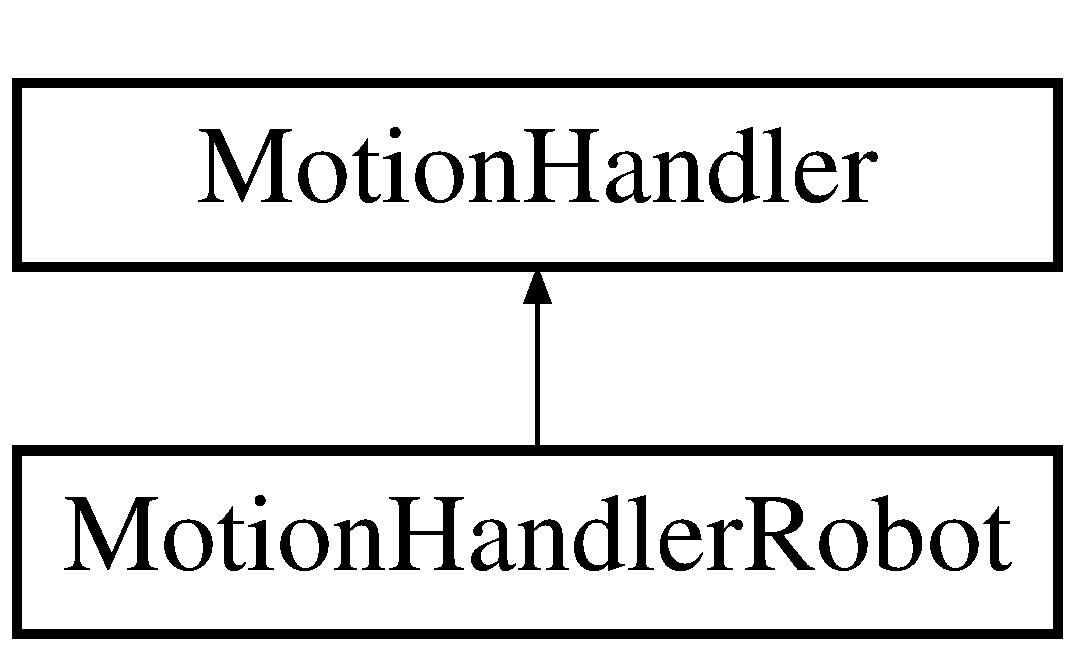
\includegraphics[height=2.000000cm]{class_motion_handler}
\end{center}
\end{figure}
\subsection*{Public Member Functions}
\begin{DoxyCompactItemize}
\item 
\mbox{\Hypertarget{class_motion_handler_a48c0070bfda6acb8a7493eb7fe1200c4}\label{class_motion_handler_a48c0070bfda6acb8a7493eb7fe1200c4}} 
\mbox{\hyperlink{class_motion_handler_a48c0070bfda6acb8a7493eb7fe1200c4}{Motion\+Handler}} (\mbox{\hyperlink{class_arena_mobile_entity}{Arena\+Mobile\+Entity}} $\ast$ent)
\begin{DoxyCompactList}\small\item\em Constructor. \end{DoxyCompactList}\item 
\mbox{\Hypertarget{class_motion_handler_aeb9e090d5d5f750767ea82d604f11c9c}\label{class_motion_handler_aeb9e090d5d5f750767ea82d604f11c9c}} 
virtual \mbox{\hyperlink{class_motion_handler_aeb9e090d5d5f750767ea82d604f11c9c}{$\sim$\+Motion\+Handler}} ()
\begin{DoxyCompactList}\small\item\em Default destructor. \end{DoxyCompactList}\item 
\mbox{\Hypertarget{class_motion_handler_a91dc98beab9d5ccce6b6c18ce32c0488}\label{class_motion_handler_a91dc98beab9d5ccce6b6c18ce32c0488}} 
\mbox{\hyperlink{class_motion_handler_a91dc98beab9d5ccce6b6c18ce32c0488}{Motion\+Handler}} (const \mbox{\hyperlink{class_motion_handler}{Motion\+Handler}} \&other)=default
\begin{DoxyCompactList}\small\item\em Default copy constructor. \end{DoxyCompactList}\item 
\mbox{\Hypertarget{class_motion_handler_ad45188f2d9794fd2b257d586a7b522e6}\label{class_motion_handler_ad45188f2d9794fd2b257d586a7b522e6}} 
\mbox{\hyperlink{class_motion_handler}{Motion\+Handler}} \& \mbox{\hyperlink{class_motion_handler_ad45188f2d9794fd2b257d586a7b522e6}{operator=}} (const \mbox{\hyperlink{class_motion_handler}{Motion\+Handler}} \&other)=default
\begin{DoxyCompactList}\small\item\em Default assignment operator overload. \end{DoxyCompactList}\item 
\mbox{\Hypertarget{class_motion_handler_a1f2d27b1f7032c40b72a50757146722d}\label{class_motion_handler_a1f2d27b1f7032c40b72a50757146722d}} 
virtual void \mbox{\hyperlink{class_motion_handler_a1f2d27b1f7032c40b72a50757146722d}{Update\+Velocity}} (\mbox{\hyperlink{common_8h_a2e3484535ee610c8e19e9859563abe48}{\+\_\+\+\_\+unused}} double left\+\_\+reading, \mbox{\hyperlink{common_8h_a2e3484535ee610c8e19e9859563abe48}{\+\_\+\+\_\+unused}} double right\+\_\+reading)
\begin{DoxyCompactList}\small\item\em Update velocity based on behavior. \end{DoxyCompactList}\item 
\mbox{\Hypertarget{class_motion_handler_adcd31df93aaad96ffd8d59aa342c7aff}\label{class_motion_handler_adcd31df93aaad96ffd8d59aa342c7aff}} 
virtual void {\bfseries Update\+Velocity} (\mbox{\hyperlink{common_8h_a2e3484535ee610c8e19e9859563abe48}{\+\_\+\+\_\+unused}} double left\+\_\+light\+\_\+reading, \mbox{\hyperlink{common_8h_a2e3484535ee610c8e19e9859563abe48}{\+\_\+\+\_\+unused}} double right\+\_\+light\+\_\+reading, \mbox{\hyperlink{common_8h_a2e3484535ee610c8e19e9859563abe48}{\+\_\+\+\_\+unused}} double left\+\_\+food\+\_\+reading, \mbox{\hyperlink{common_8h_a2e3484535ee610c8e19e9859563abe48}{\+\_\+\+\_\+unused}} double right\+\_\+food\+\_\+reading)
\item 
\mbox{\Hypertarget{class_motion_handler_ada53f0d6e25d759fc3f45cc55d440177}\label{class_motion_handler_ada53f0d6e25d759fc3f45cc55d440177}} 
double \mbox{\hyperlink{class_motion_handler_ada53f0d6e25d759fc3f45cc55d440177}{get\+\_\+speed\+\_\+delta}} () const
\begin{DoxyCompactList}\small\item\em Getter for speed delta used when user requests speed increase. \end{DoxyCompactList}\item 
\mbox{\Hypertarget{class_motion_handler_a908b330346b3fe969684106bd5c7619d}\label{class_motion_handler_a908b330346b3fe969684106bd5c7619d}} 
void \mbox{\hyperlink{class_motion_handler_a908b330346b3fe969684106bd5c7619d}{set\+\_\+speed\+\_\+delta}} (double sd)
\begin{DoxyCompactList}\small\item\em Setter method for the speed delta. Set at initialization only. \end{DoxyCompactList}\item 
\mbox{\Hypertarget{class_motion_handler_aa5ec33068c516234a6521de356b08d68}\label{class_motion_handler_aa5ec33068c516234a6521de356b08d68}} 
double \mbox{\hyperlink{class_motion_handler_aa5ec33068c516234a6521de356b08d68}{get\+\_\+angle\+\_\+delta}} () const
\begin{DoxyCompactList}\small\item\em Getter for angle delta used when user requests turning. \end{DoxyCompactList}\item 
\mbox{\Hypertarget{class_motion_handler_a8c2811ddf1a0f077fec829c460009286}\label{class_motion_handler_a8c2811ddf1a0f077fec829c460009286}} 
void \mbox{\hyperlink{class_motion_handler_a8c2811ddf1a0f077fec829c460009286}{set\+\_\+angle\+\_\+delta}} (double ad)
\begin{DoxyCompactList}\small\item\em Setter method for the angle delta. Set at initialization only. \end{DoxyCompactList}\item 
\mbox{\Hypertarget{class_motion_handler_a71e2e4cdddfb8c49eb18cf41878a08c0}\label{class_motion_handler_a71e2e4cdddfb8c49eb18cf41878a08c0}} 
double \mbox{\hyperlink{class_motion_handler_a71e2e4cdddfb8c49eb18cf41878a08c0}{get\+\_\+max\+\_\+speed}} () const
\begin{DoxyCompactList}\small\item\em Getter method for the maximum speed of entity. \end{DoxyCompactList}\item 
\mbox{\Hypertarget{class_motion_handler_a32e832d35e73e9db85c16b3ff569196e}\label{class_motion_handler_a32e832d35e73e9db85c16b3ff569196e}} 
void \mbox{\hyperlink{class_motion_handler_a32e832d35e73e9db85c16b3ff569196e}{set\+\_\+max\+\_\+speed}} (double ms)
\begin{DoxyCompactList}\small\item\em Setter method for the maximum speed. Set at initialization only. \end{DoxyCompactList}\item 
\mbox{\Hypertarget{class_motion_handler_af6ef42cdbf31ec1589e14d5dfd639d79}\label{class_motion_handler_af6ef42cdbf31ec1589e14d5dfd639d79}} 
double \mbox{\hyperlink{class_motion_handler_af6ef42cdbf31ec1589e14d5dfd639d79}{get\+\_\+max\+\_\+angle}} () const
\begin{DoxyCompactList}\small\item\em Getter method for the maximum angle. \end{DoxyCompactList}\item 
\mbox{\Hypertarget{class_motion_handler_aa73973c705626f1f95ac59391f23bcc9}\label{class_motion_handler_aa73973c705626f1f95ac59391f23bcc9}} 
void \mbox{\hyperlink{class_motion_handler_aa73973c705626f1f95ac59391f23bcc9}{set\+\_\+max\+\_\+angle}} (double ma)
\begin{DoxyCompactList}\small\item\em Setter method for the maximum angle. Set at initialization only. \end{DoxyCompactList}\item 
\mbox{\Hypertarget{class_motion_handler_abe03a52474984233d1867405925a4102}\label{class_motion_handler_abe03a52474984233d1867405925a4102}} 
\mbox{\hyperlink{struct_wheel_velocity}{Wheel\+Velocity}} \mbox{\hyperlink{class_motion_handler_abe03a52474984233d1867405925a4102}{get\+\_\+velocity}} () const
\begin{DoxyCompactList}\small\item\em Getter for \mbox{\hyperlink{struct_wheel_velocity}{Wheel\+Velocity}} struct, which has a .left and .right value. \end{DoxyCompactList}\item 
\mbox{\Hypertarget{class_motion_handler_ac4bf67ba783c1afb5a5839229de3f3f9}\label{class_motion_handler_ac4bf67ba783c1afb5a5839229de3f3f9}} 
void \mbox{\hyperlink{class_motion_handler_ac4bf67ba783c1afb5a5839229de3f3f9}{set\+\_\+velocity}} (\mbox{\hyperlink{struct_wheel_velocity}{Wheel\+Velocity}} vel)
\begin{DoxyCompactList}\small\item\em Setter for \mbox{\hyperlink{struct_wheel_velocity}{Wheel\+Velocity}} struct with struct as input param. \end{DoxyCompactList}\item 
\mbox{\Hypertarget{class_motion_handler_af31975aa667ca20835e4d5bb0216706e}\label{class_motion_handler_af31975aa667ca20835e4d5bb0216706e}} 
void \mbox{\hyperlink{class_motion_handler_af31975aa667ca20835e4d5bb0216706e}{set\+\_\+velocity}} (double vl, double vr)
\begin{DoxyCompactList}\small\item\em Setter for \mbox{\hyperlink{struct_wheel_velocity}{Wheel\+Velocity}} struct with input params of .left and .right components. \end{DoxyCompactList}\item 
\mbox{\Hypertarget{class_motion_handler_ad8472612d15be1ada7f919f45d245adc}\label{class_motion_handler_ad8472612d15be1ada7f919f45d245adc}} 
\mbox{\hyperlink{class_arena_mobile_entity}{Arena\+Mobile\+Entity}} $\ast$ \mbox{\hyperlink{class_motion_handler_ad8472612d15be1ada7f919f45d245adc}{get\+\_\+entity}} ()
\begin{DoxyCompactList}\small\item\em Return the entity. \end{DoxyCompactList}\end{DoxyCompactItemize}
\subsection*{Protected Attributes}
\begin{DoxyCompactItemize}
\item 
\mbox{\Hypertarget{class_motion_handler_a659fd1ec8878260a63779bf45681f5a4}\label{class_motion_handler_a659fd1ec8878260a63779bf45681f5a4}} 
\mbox{\hyperlink{class_arena_mobile_entity}{Arena\+Mobile\+Entity}} $\ast$ {\bfseries entity\+\_\+}
\end{DoxyCompactItemize}


\subsection{Detailed Description}
\mbox{\hyperlink{class_food}{Food}} class for managing the pose and wheel velocity of the entity. 

The pose.\+heading will change when the entity collides. The pose position will change at each timestep, which is determined by the motion behavior, not the handler. The pose.\+heading might change at each timestep (if wheel velocities are not equivalent), again determined by the motion behavior. 

The documentation for this class was generated from the following file\+:\begin{DoxyCompactItemize}
\item 
src/\mbox{\hyperlink{motion__handler_8h}{motion\+\_\+handler.\+h}}\end{DoxyCompactItemize}

\hypertarget{class_motion_handler_robot}{}\section{Motion\+Handler\+Robot Class Reference}
\label{class_motion_handler_robot}\index{Motion\+Handler\+Robot@{Motion\+Handler\+Robot}}


Class managing a \mbox{\hyperlink{class_robot}{Robot}}\textquotesingle{}s speed and heading angle foodd on collisions and user inputs.  




{\ttfamily \#include $<$motion\+\_\+handler\+\_\+robot.\+h$>$}

Inheritance diagram for Motion\+Handler\+Robot\+:\begin{figure}[H]
\begin{center}
\leavevmode
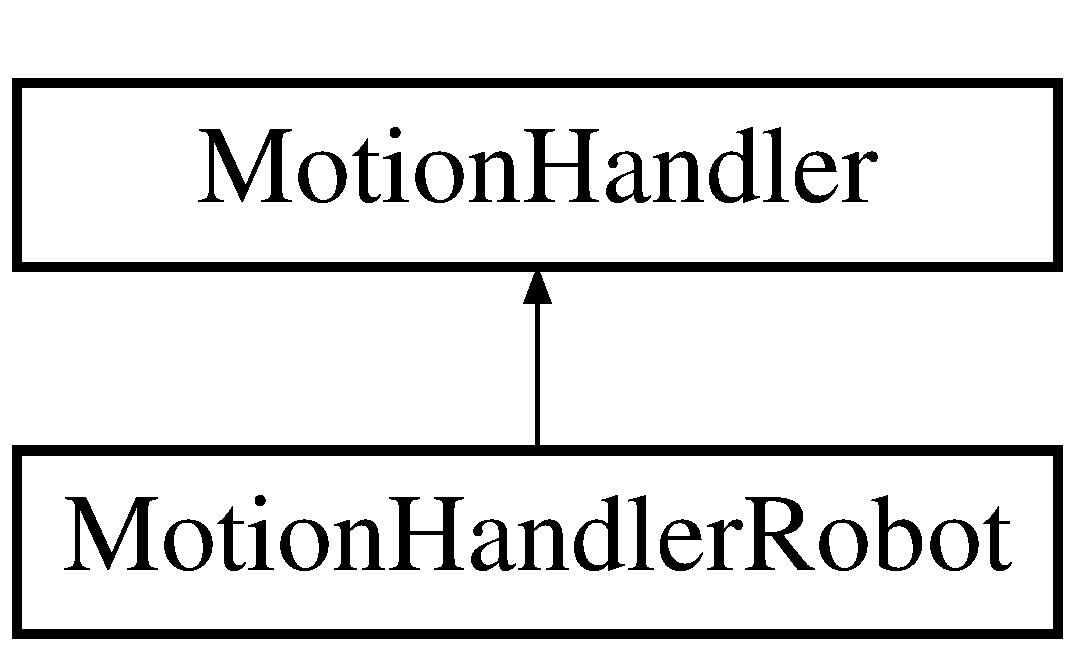
\includegraphics[height=2.000000cm]{class_motion_handler_robot}
\end{center}
\end{figure}
\subsection*{Public Member Functions}
\begin{DoxyCompactItemize}
\item 
\mbox{\Hypertarget{class_motion_handler_robot_a000adbb625eb8954e648d0f14afa7b12}\label{class_motion_handler_robot_a000adbb625eb8954e648d0f14afa7b12}} 
\mbox{\hyperlink{class_motion_handler_robot_a000adbb625eb8954e648d0f14afa7b12}{Motion\+Handler\+Robot}} (\mbox{\hyperlink{class_arena_mobile_entity}{Arena\+Mobile\+Entity}} $\ast$ent, Behavior behavior)
\begin{DoxyCompactList}\small\item\em Explicit value constructor. \end{DoxyCompactList}\item 
\mbox{\Hypertarget{class_motion_handler_robot_a66445cc9057e3ef9298b5bd239df6d4e}\label{class_motion_handler_robot_a66445cc9057e3ef9298b5bd239df6d4e}} 
\mbox{\hyperlink{class_motion_handler_robot_a66445cc9057e3ef9298b5bd239df6d4e}{Motion\+Handler\+Robot}} (const \mbox{\hyperlink{class_motion_handler_robot}{Motion\+Handler\+Robot}} \&other)=default
\begin{DoxyCompactList}\small\item\em Default copy constructor. \end{DoxyCompactList}\item 
\mbox{\Hypertarget{class_motion_handler_robot_a48181f197ffb864f16e29721ad964e4a}\label{class_motion_handler_robot_a48181f197ffb864f16e29721ad964e4a}} 
\mbox{\hyperlink{class_motion_handler_robot}{Motion\+Handler\+Robot}} \& \mbox{\hyperlink{class_motion_handler_robot_a48181f197ffb864f16e29721ad964e4a}{operator=}} (const \mbox{\hyperlink{class_motion_handler_robot}{Motion\+Handler\+Robot}} \&other)=default
\begin{DoxyCompactList}\small\item\em Default assignment operator overload. \end{DoxyCompactList}\item 
void \mbox{\hyperlink{class_motion_handler_robot_aba3ad202a5dc1cf13dc1a82308776ecf}{Update\+Velocity}} (double left\+\_\+reading, double right\+\_\+reading) override
\begin{DoxyCompactList}\small\item\em Set the speed of both wheels based upon the robots proximity to the light. \end{DoxyCompactList}\item 
void \mbox{\hyperlink{class_motion_handler_robot_a2afe4dbe1eb88998442f6f41ce8f0c2c}{Update\+Velocity}} (double left\+\_\+light\+\_\+reading, double right\+\_\+light\+\_\+reading, double left\+\_\+food\+\_\+reading, double right\+\_\+food\+\_\+reading) override
\begin{DoxyCompactList}\small\item\em Set the speed of both wheels based upon the robots proximity to the food and the light. \end{DoxyCompactList}\item 
void \mbox{\hyperlink{class_motion_handler_robot_accf55d58d0ddae44c4e054f7784b9e9a}{set\+\_\+behavior}} (Behavior behavior)
\begin{DoxyCompactList}\small\item\em Set the type of braitenberg vehicle based upon the behavior. \end{DoxyCompactList}\end{DoxyCompactItemize}
\subsection*{Additional Inherited Members}


\subsection{Detailed Description}
Class managing a \mbox{\hyperlink{class_robot}{Robot}}\textquotesingle{}s speed and heading angle foodd on collisions and user inputs. 

Currently, both wheels are always going at maximum speed, and cannot be controlled independently. 

\subsection{Member Function Documentation}
\mbox{\Hypertarget{class_motion_handler_robot_accf55d58d0ddae44c4e054f7784b9e9a}\label{class_motion_handler_robot_accf55d58d0ddae44c4e054f7784b9e9a}} 
\index{Motion\+Handler\+Robot@{Motion\+Handler\+Robot}!set\+\_\+behavior@{set\+\_\+behavior}}
\index{set\+\_\+behavior@{set\+\_\+behavior}!Motion\+Handler\+Robot@{Motion\+Handler\+Robot}}
\subsubsection{\texorpdfstring{set\+\_\+behavior()}{set\_behavior()}}
{\footnotesize\ttfamily void Motion\+Handler\+Robot\+::set\+\_\+behavior (\begin{DoxyParamCaption}\item[{Behavior}]{behavior }\end{DoxyParamCaption})}



Set the type of braitenberg vehicle based upon the behavior. 


\begin{DoxyParams}{Parameters}
{\em behavior} & -\/ The way the robot will move based upon the entities \\
\hline
\end{DoxyParams}
\mbox{\Hypertarget{class_motion_handler_robot_aba3ad202a5dc1cf13dc1a82308776ecf}\label{class_motion_handler_robot_aba3ad202a5dc1cf13dc1a82308776ecf}} 
\index{Motion\+Handler\+Robot@{Motion\+Handler\+Robot}!Update\+Velocity@{Update\+Velocity}}
\index{Update\+Velocity@{Update\+Velocity}!Motion\+Handler\+Robot@{Motion\+Handler\+Robot}}
\subsubsection{\texorpdfstring{Update\+Velocity()}{UpdateVelocity()}\hspace{0.1cm}{\footnotesize\ttfamily [1/2]}}
{\footnotesize\ttfamily void Motion\+Handler\+Robot\+::\+Update\+Velocity (\begin{DoxyParamCaption}\item[{double}]{left\+\_\+reading,  }\item[{double}]{right\+\_\+reading }\end{DoxyParamCaption})\hspace{0.3cm}{\ttfamily [override]}}



Set the speed of both wheels based upon the robots proximity to the light. 


\begin{DoxyParams}[1]{Parameters}
\mbox{\tt in}  & {\em left\+\_\+reading} & -\/ reading for the sensor on the left \\
\hline
\mbox{\tt in}  & {\em right\+\_\+reading} & -\/ reading for the sensor on the right \\
\hline
\mbox{\tt out}  & {\em The} & proper wheel velocities \\
\hline
\end{DoxyParams}
\mbox{\Hypertarget{class_motion_handler_robot_a2afe4dbe1eb88998442f6f41ce8f0c2c}\label{class_motion_handler_robot_a2afe4dbe1eb88998442f6f41ce8f0c2c}} 
\index{Motion\+Handler\+Robot@{Motion\+Handler\+Robot}!Update\+Velocity@{Update\+Velocity}}
\index{Update\+Velocity@{Update\+Velocity}!Motion\+Handler\+Robot@{Motion\+Handler\+Robot}}
\subsubsection{\texorpdfstring{Update\+Velocity()}{UpdateVelocity()}\hspace{0.1cm}{\footnotesize\ttfamily [2/2]}}
{\footnotesize\ttfamily void Motion\+Handler\+Robot\+::\+Update\+Velocity (\begin{DoxyParamCaption}\item[{double}]{left\+\_\+light\+\_\+reading,  }\item[{double}]{right\+\_\+light\+\_\+reading,  }\item[{double}]{left\+\_\+food\+\_\+reading,  }\item[{double}]{right\+\_\+food\+\_\+reading }\end{DoxyParamCaption})\hspace{0.3cm}{\ttfamily [override]}}



Set the speed of both wheels based upon the robots proximity to the food and the light. 


\begin{DoxyParams}[1]{Parameters}
\mbox{\tt in}  & {\em left\+\_\+light\+\_\+reading} & -\/ reading for light sensor on the left \\
\hline
\mbox{\tt in}  & {\em right\+\_\+light\+\_\+reading} & -\/ reading for light sensor on the right \\
\hline
\mbox{\tt in}  & {\em left\+\_\+food\+\_\+reading} & -\/ reading for food sensor on the left \\
\hline
\mbox{\tt in}  & {\em right\+\_\+food\+\_\+reading} & -\/ reading for food sensor on the right \\
\hline
\mbox{\tt out}  & {\em The} & proper wheel velocities \\
\hline
\end{DoxyParams}


The documentation for this class was generated from the following files\+:\begin{DoxyCompactItemize}
\item 
src/\mbox{\hyperlink{motion__handler__robot_8h}{motion\+\_\+handler\+\_\+robot.\+h}}\item 
src/\mbox{\hyperlink{motion__handler__robot_8cc}{motion\+\_\+handler\+\_\+robot.\+cc}}\end{DoxyCompactItemize}

\hypertarget{struct_pose}{}\section{Pose Struct Reference}
\label{struct_pose}\index{Pose@{Pose}}


A simple representation of the position/orientation of an entity within the \mbox{\hyperlink{class_arena}{Arena}}.  




{\ttfamily \#include $<$pose.\+h$>$}

\subsection*{Public Member Functions}
\begin{DoxyCompactItemize}
\item 
\mbox{\Hypertarget{struct_pose_a8a4171c8a6b09e37fb011997da9ea2ad}\label{struct_pose_a8a4171c8a6b09e37fb011997da9ea2ad}} 
\mbox{\hyperlink{struct_pose_a8a4171c8a6b09e37fb011997da9ea2ad}{Pose}} ()
\begin{DoxyCompactList}\small\item\em Default constructor. Initialize the pose to (0,0,0) \end{DoxyCompactList}\item 
\mbox{\hyperlink{struct_pose_ac947d7046547d883f782ab2408cb80ed}{Pose}} (double in\+\_\+x, double in\+\_\+y)
\begin{DoxyCompactList}\small\item\em Constructor. \end{DoxyCompactList}\item 
\mbox{\Hypertarget{struct_pose_a6ebb8a1510c5915fa1dbec0f7ba0ad1c}\label{struct_pose_a6ebb8a1510c5915fa1dbec0f7ba0ad1c}} 
{\bfseries Pose} (double in\+\_\+x, double in\+\_\+y, double in\+\_\+theta)
\item 
\mbox{\hyperlink{struct_pose}{Pose}} \& \mbox{\hyperlink{struct_pose_aec0a9478daefa358aa2f1873cbaf0271}{operator=}} (const \mbox{\hyperlink{struct_pose}{Pose}} \&other)=default
\begin{DoxyCompactList}\small\item\em Default assignment operator. Simply copies the (x,y) values of another \mbox{\hyperlink{struct_pose}{Pose}}. \end{DoxyCompactList}\end{DoxyCompactItemize}
\subsection*{Public Attributes}
\begin{DoxyCompactItemize}
\item 
\mbox{\Hypertarget{struct_pose_a0061c7789df90f593ab95118cbef387f}\label{struct_pose_a0061c7789df90f593ab95118cbef387f}} 
double {\bfseries x} \{0\}
\item 
\mbox{\Hypertarget{struct_pose_a6280216efe0840a7a55f025ad04e3b3d}\label{struct_pose_a6280216efe0840a7a55f025ad04e3b3d}} 
double {\bfseries y} \{0\}
\item 
\mbox{\Hypertarget{struct_pose_a25709c116282114c9f512b205f3f1133}\label{struct_pose_a25709c116282114c9f512b205f3f1133}} 
double {\bfseries theta} \{0.\+0\}
\end{DoxyCompactItemize}


\subsection{Detailed Description}
A simple representation of the position/orientation of an entity within the \mbox{\hyperlink{class_arena}{Arena}}. 

N\+O\+TE\+: Origin (0,0) is at the upper left corner of the \mbox{\hyperlink{class_arena}{Arena}}. 

\subsection{Constructor \& Destructor Documentation}
\mbox{\Hypertarget{struct_pose_ac947d7046547d883f782ab2408cb80ed}\label{struct_pose_ac947d7046547d883f782ab2408cb80ed}} 
\index{Pose@{Pose}!Pose@{Pose}}
\index{Pose@{Pose}!Pose@{Pose}}
\subsubsection{\texorpdfstring{Pose()}{Pose()}}
{\footnotesize\ttfamily Pose\+::\+Pose (\begin{DoxyParamCaption}\item[{double}]{in\+\_\+x,  }\item[{double}]{in\+\_\+y }\end{DoxyParamCaption})\hspace{0.3cm}{\ttfamily [inline]}}



Constructor. 


\begin{DoxyParams}{Parameters}
{\em in\+\_\+x} & The X component of the \mbox{\hyperlink{struct_pose}{Pose}}. \\
\hline
{\em in\+\_\+y} & The Y component of the \mbox{\hyperlink{struct_pose}{Pose}}. \\
\hline
\end{DoxyParams}


\subsection{Member Function Documentation}
\mbox{\Hypertarget{struct_pose_aec0a9478daefa358aa2f1873cbaf0271}\label{struct_pose_aec0a9478daefa358aa2f1873cbaf0271}} 
\index{Pose@{Pose}!operator=@{operator=}}
\index{operator=@{operator=}!Pose@{Pose}}
\subsubsection{\texorpdfstring{operator=()}{operator=()}}
{\footnotesize\ttfamily \mbox{\hyperlink{struct_pose}{Pose}}\& Pose\+::operator= (\begin{DoxyParamCaption}\item[{const \mbox{\hyperlink{struct_pose}{Pose}} \&}]{other }\end{DoxyParamCaption})\hspace{0.3cm}{\ttfamily [default]}}



Default assignment operator. Simply copies the (x,y) values of another \mbox{\hyperlink{struct_pose}{Pose}}. 


\begin{DoxyParams}{Parameters}
{\em other} & The \mbox{\hyperlink{struct_pose}{Pose}} object to copy from.\\
\hline
\end{DoxyParams}
\begin{DoxyReturn}{Returns}
The left-\/hand-\/side \mbox{\hyperlink{struct_pose}{Pose}} object that is now identical (in value) to {\ttfamily other}. 
\end{DoxyReturn}


The documentation for this struct was generated from the following file\+:\begin{DoxyCompactItemize}
\item 
src/\mbox{\hyperlink{pose_8h}{pose.\+h}}\end{DoxyCompactItemize}

\hypertarget{struct_rgb_color}{}\section{Rgb\+Color Struct Reference}
\label{struct_rgb_color}\index{Rgb\+Color@{Rgb\+Color}}


Struct representing a rgb\+\_\+color.  




{\ttfamily \#include $<$rgb\+\_\+color.\+h$>$}

\subsection*{Public Member Functions}
\begin{DoxyCompactItemize}
\item 
\mbox{\hyperlink{struct_rgb_color_a264da0270aca412d62197e046b71b08e}{Rgb\+Color}} ()
\begin{DoxyCompactList}\small\item\em Default constructor. \end{DoxyCompactList}\item 
\mbox{\hyperlink{struct_rgb_color_a61e213533bfff019aebd27f991688222}{Rgb\+Color}} (int r\+\_\+in, int g\+\_\+in, int b\+\_\+in)
\begin{DoxyCompactList}\small\item\em Constructor for Rgb\+\_\+\+Color. \end{DoxyCompactList}\item 
\mbox{\Hypertarget{struct_rgb_color_a57fcd9161e0ee6a38e707c5002db55b8}\label{struct_rgb_color_a57fcd9161e0ee6a38e707c5002db55b8}} 
void {\bfseries Set} (Rgb\+Color\+Enum value)
\end{DoxyCompactItemize}
\subsection*{Public Attributes}
\begin{DoxyCompactItemize}
\item 
\mbox{\Hypertarget{struct_rgb_color_aa6c2fac108029c79f7cc96fb6d34717f}\label{struct_rgb_color_aa6c2fac108029c79f7cc96fb6d34717f}} 
int {\bfseries r} \{0\}
\item 
\mbox{\Hypertarget{struct_rgb_color_afbc54745bd4ed7ede168e31922143eff}\label{struct_rgb_color_afbc54745bd4ed7ede168e31922143eff}} 
int {\bfseries g} \{0\}
\item 
\mbox{\Hypertarget{struct_rgb_color_af1ba4837230cfc3b0f31454ccdb03df6}\label{struct_rgb_color_af1ba4837230cfc3b0f31454ccdb03df6}} 
int {\bfseries b} \{0\}
\end{DoxyCompactItemize}


\subsection{Detailed Description}
Struct representing a rgb\+\_\+color. 

Internally uses R\+G\+BA values to represent the rgb\+\_\+color. 

\subsection{Constructor \& Destructor Documentation}
\mbox{\Hypertarget{struct_rgb_color_a264da0270aca412d62197e046b71b08e}\label{struct_rgb_color_a264da0270aca412d62197e046b71b08e}} 
\index{Rgb\+Color@{Rgb\+Color}!Rgb\+Color@{Rgb\+Color}}
\index{Rgb\+Color@{Rgb\+Color}!Rgb\+Color@{Rgb\+Color}}
\subsubsection{\texorpdfstring{Rgb\+Color()}{RgbColor()}\hspace{0.1cm}{\footnotesize\ttfamily [1/2]}}
{\footnotesize\ttfamily Rgb\+Color\+::\+Rgb\+Color (\begin{DoxyParamCaption}{ }\end{DoxyParamCaption})\hspace{0.3cm}{\ttfamily [inline]}}



Default constructor. 

Initialize R\+GB all to 0 (k\+White). \mbox{\Hypertarget{struct_rgb_color_a61e213533bfff019aebd27f991688222}\label{struct_rgb_color_a61e213533bfff019aebd27f991688222}} 
\index{Rgb\+Color@{Rgb\+Color}!Rgb\+Color@{Rgb\+Color}}
\index{Rgb\+Color@{Rgb\+Color}!Rgb\+Color@{Rgb\+Color}}
\subsubsection{\texorpdfstring{Rgb\+Color()}{RgbColor()}\hspace{0.1cm}{\footnotesize\ttfamily [2/2]}}
{\footnotesize\ttfamily Rgb\+Color\+::\+Rgb\+Color (\begin{DoxyParamCaption}\item[{int}]{r\+\_\+in,  }\item[{int}]{g\+\_\+in,  }\item[{int}]{b\+\_\+in }\end{DoxyParamCaption})\hspace{0.3cm}{\ttfamily [inline]}}



Constructor for Rgb\+\_\+\+Color. 


\begin{DoxyParams}{Parameters}
{\em r\+\_\+in} & The R component of the rgb\+\_\+color. \\
\hline
{\em g\+\_\+in} & The G component of the rgb\+\_\+color. \\
\hline
{\em b\+\_\+in} & The B component of the rgb\+\_\+color. \\
\hline
\end{DoxyParams}


The documentation for this struct was generated from the following files\+:\begin{DoxyCompactItemize}
\item 
src/\mbox{\hyperlink{rgb__color_8h}{rgb\+\_\+color.\+h}}\item 
src/\mbox{\hyperlink{rgb__color_8cc}{rgb\+\_\+color.\+cc}}\end{DoxyCompactItemize}

\hypertarget{class_robot}{}\section{Robot Class Reference}
\label{class_robot}\index{Robot@{Robot}}


Class representing a robot within the arena.  




{\ttfamily \#include $<$robot.\+h$>$}

Inheritance diagram for Robot\+:\begin{figure}[H]
\begin{center}
\leavevmode
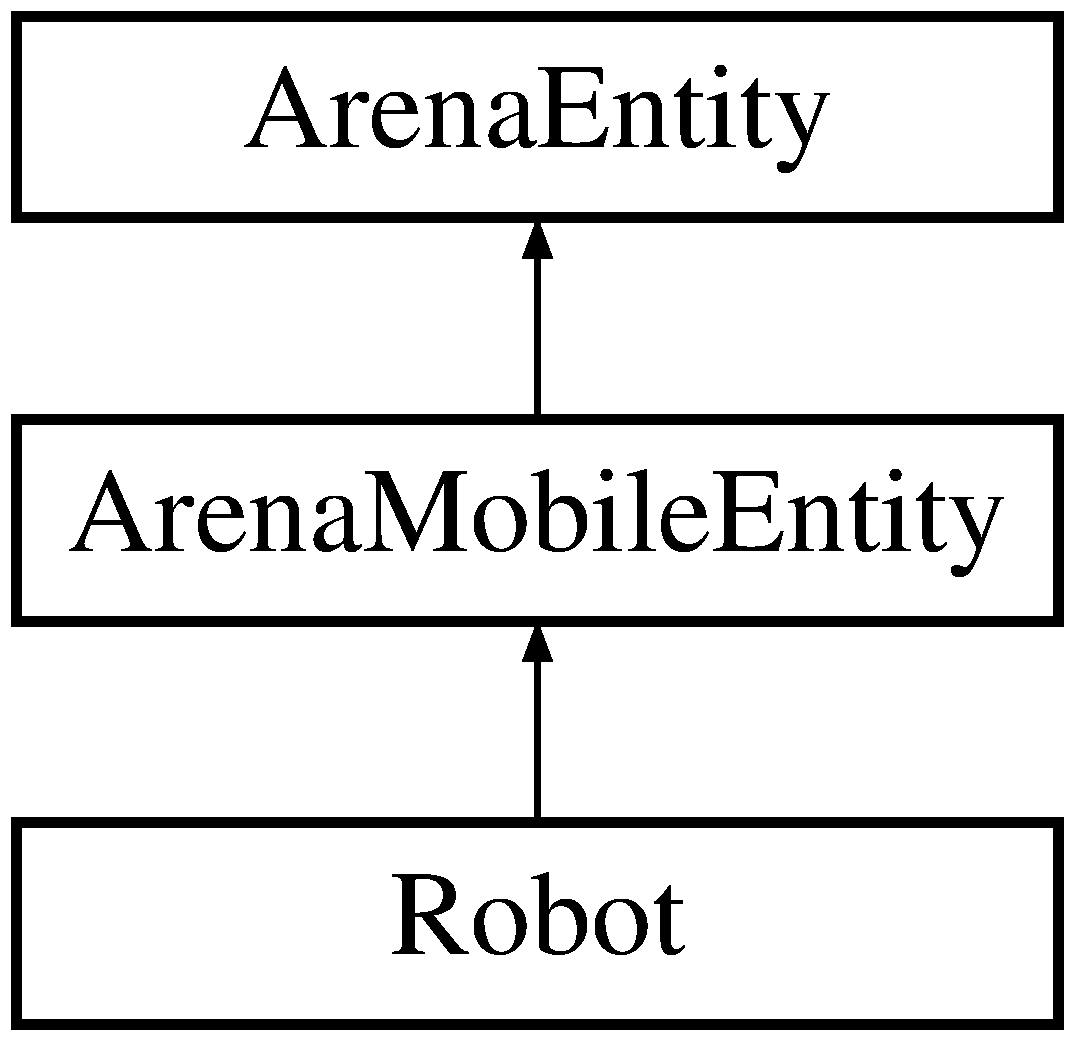
\includegraphics[height=3.000000cm]{class_robot}
\end{center}
\end{figure}
\subsection*{Public Member Functions}
\begin{DoxyCompactItemize}
\item 
\mbox{\Hypertarget{class_robot_afc21c5c822196c987a73d35d02c0c26d}\label{class_robot_afc21c5c822196c987a73d35d02c0c26d}} 
\mbox{\hyperlink{class_robot_afc21c5c822196c987a73d35d02c0c26d}{Robot}} (Behavior behavior)
\begin{DoxyCompactList}\small\item\em Constructor using initialization values from \mbox{\hyperlink{params_8h}{params.\+h}}. \end{DoxyCompactList}\item 
\mbox{\Hypertarget{class_robot_a4ed87722425dbfdc35631a0b8b58859f}\label{class_robot_a4ed87722425dbfdc35631a0b8b58859f}} 
virtual \mbox{\hyperlink{class_robot_a4ed87722425dbfdc35631a0b8b58859f}{$\sim$\+Robot}} ()=default
\begin{DoxyCompactList}\small\item\em Default destructor. \end{DoxyCompactList}\item 
\mbox{\Hypertarget{class_robot_a69f171c4965ac4523cd95e2191405d37}\label{class_robot_a69f171c4965ac4523cd95e2191405d37}} 
\mbox{\hyperlink{class_robot}{Robot}} \& \mbox{\hyperlink{class_robot_a69f171c4965ac4523cd95e2191405d37}{operator=}} (const \mbox{\hyperlink{class_robot}{Robot}} \&other)=default
\begin{DoxyCompactList}\small\item\em Default assignment operator overload. \end{DoxyCompactList}\item 
\mbox{\Hypertarget{class_robot_a87ee951bb2c663a8bb427fdd2928a934}\label{class_robot_a87ee951bb2c663a8bb427fdd2928a934}} 
\mbox{\hyperlink{class_robot_a87ee951bb2c663a8bb427fdd2928a934}{Robot}} (const \mbox{\hyperlink{class_robot}{Robot}} \&other)=default
\begin{DoxyCompactList}\small\item\em Default copy constructor. \end{DoxyCompactList}\item 
\mbox{\Hypertarget{class_robot_af597fd14927d2cd5308ded62f4e54e29}\label{class_robot_af597fd14927d2cd5308ded62f4e54e29}} 
void \mbox{\hyperlink{class_robot_af597fd14927d2cd5308ded62f4e54e29}{Reset}} () override
\begin{DoxyCompactList}\small\item\em Reset the \mbox{\hyperlink{class_robot}{Robot}} to a newly constructed state (needed for reset button to work in G\+UI). \end{DoxyCompactList}\item 
void \mbox{\hyperlink{class_robot_ae790462f8782efcfd26082eedec30ed5}{Timestep\+Update}} (unsigned int dt) override
\begin{DoxyCompactList}\small\item\em Update the \mbox{\hyperlink{class_robot}{Robot}}\textquotesingle{}s position and velocity after the specified duration has passed. \end{DoxyCompactList}\item 
\mbox{\Hypertarget{class_robot_a176a9958cc2ea1e585ddb2cdc82c0bdb}\label{class_robot_a176a9958cc2ea1e585ddb2cdc82c0bdb}} 
void \mbox{\hyperlink{class_robot_a176a9958cc2ea1e585ddb2cdc82c0bdb}{Handle\+Collision}} (Entity\+Type object\+\_\+type, \mbox{\hyperlink{class_arena_entity}{Arena\+Entity}} $\ast$object=N\+U\+LL)
\begin{DoxyCompactList}\small\item\em Handles the collision by setting the sensor to activated. \end{DoxyCompactList}\item 
\mbox{\Hypertarget{class_robot_a3f77c13705b8f60480d21d8d936dc39e}\label{class_robot_a3f77c13705b8f60480d21d8d936dc39e}} 
std\+::string \mbox{\hyperlink{class_robot_a3f77c13705b8f60480d21d8d936dc39e}{get\+\_\+name}} () const override
\begin{DoxyCompactList}\small\item\em Get the name of the \mbox{\hyperlink{class_robot}{Robot}} for visualization and for debugging. \end{DoxyCompactList}\item 
\mbox{\Hypertarget{class_robot_a77d37cf0058d18b7f633202e8c1bf814}\label{class_robot_a77d37cf0058d18b7f633202e8c1bf814}} 
\mbox{\hyperlink{class_motion_handler_robot}{Motion\+Handler\+Robot}} \mbox{\hyperlink{class_robot_a77d37cf0058d18b7f633202e8c1bf814}{get\+\_\+motion\+\_\+handler}} ()
\begin{DoxyCompactList}\small\item\em Return the motion\+\_\+handler\+\_\+ and its functions. \end{DoxyCompactList}\item 
\mbox{\Hypertarget{class_robot_ab45bf3c6fdafcd14cdbdb2a8e3f558b8}\label{class_robot_ab45bf3c6fdafcd14cdbdb2a8e3f558b8}} 
\mbox{\hyperlink{class_motion_behavior_differential}{Motion\+Behavior\+Differential}} \mbox{\hyperlink{class_robot_ab45bf3c6fdafcd14cdbdb2a8e3f558b8}{get\+\_\+motion\+\_\+behavior}} ()
\begin{DoxyCompactList}\small\item\em Return the motion\+\_\+behavior\+\_\+ and its functions. \end{DoxyCompactList}\item 
\mbox{\Hypertarget{class_robot_a464e8c93ec1ed8e632285c5d51777bc0}\label{class_robot_a464e8c93ec1ed8e632285c5d51777bc0}} 
void \mbox{\hyperlink{class_robot_a464e8c93ec1ed8e632285c5d51777bc0}{set\+\_\+behavior}} (Behavior behavior)
\begin{DoxyCompactList}\small\item\em Sets the robot\textquotesingle{}s behavior. \end{DoxyCompactList}\item 
\mbox{\Hypertarget{class_robot_a1277018a7a7b38353141971833367d21}\label{class_robot_a1277018a7a7b38353141971833367d21}} 
Behavior \mbox{\hyperlink{class_robot_a1277018a7a7b38353141971833367d21}{get\+\_\+behavior}} ()
\begin{DoxyCompactList}\small\item\em Return the robot behavior, foodd upon the behavior the robot will react to light in different ways. \end{DoxyCompactList}\item 
\mbox{\Hypertarget{class_robot_a11f677bb307f6b94846e5e463a1ddba2}\label{class_robot_a11f677bb307f6b94846e5e463a1ddba2}} 
\mbox{\hyperlink{class_light_sensor}{Light\+Sensor}} $\ast$ \mbox{\hyperlink{class_robot_a11f677bb307f6b94846e5e463a1ddba2}{get\+\_\+light\+\_\+sensor\+\_\+left}} () const
\begin{DoxyCompactList}\small\item\em Return the left light sensor. \end{DoxyCompactList}\item 
\mbox{\Hypertarget{class_robot_a8513b9257593c5191f776f7401b92ff3}\label{class_robot_a8513b9257593c5191f776f7401b92ff3}} 
\mbox{\hyperlink{class_light_sensor}{Light\+Sensor}} $\ast$ \mbox{\hyperlink{class_robot_a8513b9257593c5191f776f7401b92ff3}{get\+\_\+light\+\_\+sensor\+\_\+right}} () const
\begin{DoxyCompactList}\small\item\em Return the right light sensor. \end{DoxyCompactList}\item 
\mbox{\Hypertarget{class_robot_a0f3fb5482ce76b0c369870440df2766b}\label{class_robot_a0f3fb5482ce76b0c369870440df2766b}} 
\mbox{\hyperlink{class_food_sensor}{Food\+Sensor}} $\ast$ \mbox{\hyperlink{class_robot_a0f3fb5482ce76b0c369870440df2766b}{get\+\_\+food\+\_\+sensor\+\_\+left}} () const
\begin{DoxyCompactList}\small\item\em Return the right food sensor. \end{DoxyCompactList}\item 
\mbox{\Hypertarget{class_robot_a37ada921d9693a07a9160dc33e003603}\label{class_robot_a37ada921d9693a07a9160dc33e003603}} 
\mbox{\hyperlink{class_food_sensor}{Food\+Sensor}} $\ast$ \mbox{\hyperlink{class_robot_a37ada921d9693a07a9160dc33e003603}{get\+\_\+food\+\_\+sensor\+\_\+right}} () const
\begin{DoxyCompactList}\small\item\em Return the right food sensor. \end{DoxyCompactList}\item 
\mbox{\Hypertarget{class_robot_abc89e4cbfdb05d647aace0d6f8f8dfef}\label{class_robot_abc89e4cbfdb05d647aace0d6f8f8dfef}} 
void \mbox{\hyperlink{class_robot_abc89e4cbfdb05d647aace0d6f8f8dfef}{set\+\_\+hunger\+\_\+time}} (float hunger\+\_\+time)
\begin{DoxyCompactList}\small\item\em Set the robot\textquotesingle{}s hunger time. \end{DoxyCompactList}\item 
\mbox{\Hypertarget{class_robot_a9d7b6f961ed92864b61845e4a1ef06bf}\label{class_robot_a9d7b6f961ed92864b61845e4a1ef06bf}} 
float \mbox{\hyperlink{class_robot_a9d7b6f961ed92864b61845e4a1ef06bf}{get\+\_\+hunger\+\_\+time}} ()
\begin{DoxyCompactList}\small\item\em Return the hunger time. \end{DoxyCompactList}\item 
\mbox{\Hypertarget{class_robot_a10d487aa1da1887944f8982053a7ce4b}\label{class_robot_a10d487aa1da1887944f8982053a7ce4b}} 
void \mbox{\hyperlink{class_robot_a10d487aa1da1887944f8982053a7ce4b}{reset\+\_\+arc\+\_\+time}} ()
\begin{DoxyCompactList}\small\item\em Resets the arc time to the maximum. \end{DoxyCompactList}\item 
\mbox{\Hypertarget{class_robot_addffb7962b2053aa0d2499306162f092}\label{class_robot_addffb7962b2053aa0d2499306162f092}} 
void {\bfseries set\+\_\+has\+\_\+hunger} (bool has\+\_\+hunger)
\end{DoxyCompactItemize}
\subsection*{Additional Inherited Members}


\subsection{Detailed Description}
Class representing a robot within the arena. 

Robots are composed of a motion handler, motion behavior, and touch sensor. These classes interact to maintain the pose (position and heading) of the robot. At each time step, the wheel velocities are used to calculate the next pose of the robot. The handler manages the pose and user requests. The behavior calculates the new pose foodd on wheel velocities.

Robots can be controlled through keypress, which modify wheel velocities.

The touch sensor is activated when the robot collides with an object. The heading is modified after a collision to move the robot away from the other object. 

\subsection{Member Function Documentation}
\mbox{\Hypertarget{class_robot_ae790462f8782efcfd26082eedec30ed5}\label{class_robot_ae790462f8782efcfd26082eedec30ed5}} 
\index{Robot@{Robot}!Timestep\+Update@{Timestep\+Update}}
\index{Timestep\+Update@{Timestep\+Update}!Robot@{Robot}}
\subsubsection{\texorpdfstring{Timestep\+Update()}{TimestepUpdate()}}
{\footnotesize\ttfamily void Robot\+::\+Timestep\+Update (\begin{DoxyParamCaption}\item[{unsigned int}]{dt }\end{DoxyParamCaption})\hspace{0.3cm}{\ttfamily [override]}}



Update the \mbox{\hyperlink{class_robot}{Robot}}\textquotesingle{}s position and velocity after the specified duration has passed. 


\begin{DoxyParams}{Parameters}
{\em dt} & The \# of timesteps that have elapsed since the last update. \\
\hline
\end{DoxyParams}


The documentation for this class was generated from the following files\+:\begin{DoxyCompactItemize}
\item 
src/\mbox{\hyperlink{robot_8h}{robot.\+h}}\item 
src/\mbox{\hyperlink{robot_8cc}{robot.\+cc}}\end{DoxyCompactItemize}

\hypertarget{class_sensor}{}\section{Sensor Class Reference}
\label{class_sensor}\index{Sensor@{Sensor}}


Parent class for both of the sensors a robot can have.  




{\ttfamily \#include $<$sensor.\+h$>$}

Inheritance diagram for Sensor\+:\begin{figure}[H]
\begin{center}
\leavevmode
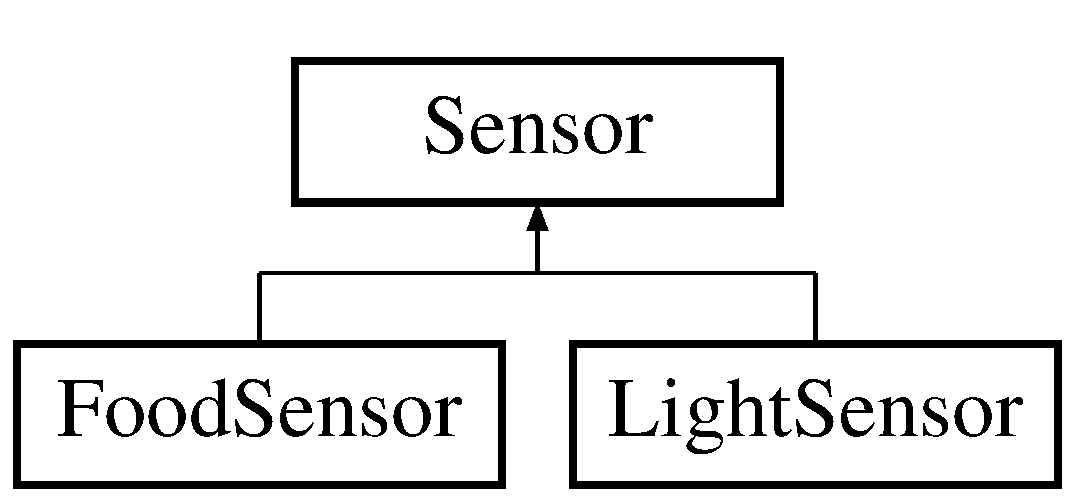
\includegraphics[height=2.000000cm]{class_sensor}
\end{center}
\end{figure}
\subsection*{Public Member Functions}
\begin{DoxyCompactItemize}
\item 
\mbox{\Hypertarget{class_sensor_a342d6d11ef572c8cba92cb76fb1a294b}\label{class_sensor_a342d6d11ef572c8cba92cb76fb1a294b}} 
\mbox{\hyperlink{class_sensor_a342d6d11ef572c8cba92cb76fb1a294b}{Sensor}} ()
\begin{DoxyCompactList}\small\item\em Default constructor. \end{DoxyCompactList}\item 
\mbox{\Hypertarget{class_sensor_a387919f060b66074dbd107ed1764f8f6}\label{class_sensor_a387919f060b66074dbd107ed1764f8f6}} 
virtual \mbox{\hyperlink{class_sensor_a387919f060b66074dbd107ed1764f8f6}{$\sim$\+Sensor}} ()=default
\begin{DoxyCompactList}\small\item\em Default destructor. \end{DoxyCompactList}\item 
double \mbox{\hyperlink{class_sensor_aab7f1f9c804ab9b05eaaa19f93b2dff7}{Calc\+Distance}} (\mbox{\hyperlink{struct_pose}{Pose}} sensor\+\_\+pose, \mbox{\hyperlink{struct_pose}{Pose}} entity\+\_\+pose)
\begin{DoxyCompactList}\small\item\em Calculates the distance between two entities. \end{DoxyCompactList}\item 
virtual void \mbox{\hyperlink{class_sensor_a8415ca43d21e24dc72481bbf1f308e5c}{Notify}} (\mbox{\hyperlink{common_8h_a2e3484535ee610c8e19e9859563abe48}{\+\_\+\+\_\+unused}} \mbox{\hyperlink{struct_pose}{Pose}} entity\+\_\+pose)
\begin{DoxyCompactList}\small\item\em Gives a sensor reading based upon the position passed in. \end{DoxyCompactList}\item 
\mbox{\Hypertarget{class_sensor_a5e6ad1aa7b2c48e59851e03404dacbde}\label{class_sensor_a5e6ad1aa7b2c48e59851e03404dacbde}} 
virtual void \mbox{\hyperlink{class_sensor_a5e6ad1aa7b2c48e59851e03404dacbde}{Reset}} ()
\begin{DoxyCompactList}\small\item\em Resets the position and the sensor reading. \end{DoxyCompactList}\item 
\mbox{\Hypertarget{class_sensor_a6ef17b207fce459422bee2410ec15c65}\label{class_sensor_a6ef17b207fce459422bee2410ec15c65}} 
\mbox{\hyperlink{class_sensor}{Sensor}} \& \mbox{\hyperlink{class_sensor_a6ef17b207fce459422bee2410ec15c65}{operator=}} (\mbox{\hyperlink{common_8h_a2e3484535ee610c8e19e9859563abe48}{\+\_\+\+\_\+unused}} const \mbox{\hyperlink{class_sensor}{Sensor}} \&other)=default
\begin{DoxyCompactList}\small\item\em Under certain circumstance, the compiler requires that the assignment operator is not defined. This {\ttfamily deletes} the default assignment operator. \end{DoxyCompactList}\item 
\mbox{\Hypertarget{class_sensor_af2e786d46a120c438bceb25a27bcbf6c}\label{class_sensor_af2e786d46a120c438bceb25a27bcbf6c}} 
\mbox{\hyperlink{class_sensor_af2e786d46a120c438bceb25a27bcbf6c}{Sensor}} (\mbox{\hyperlink{common_8h_a2e3484535ee610c8e19e9859563abe48}{\+\_\+\+\_\+unused}} const \mbox{\hyperlink{class_sensor}{Sensor}} \&other)=default
\begin{DoxyCompactList}\small\item\em Under certain circumstance, the compiler requires that the copy constructor is not defined. This {\ttfamily deletes} the default copy constructor. \end{DoxyCompactList}\item 
\mbox{\Hypertarget{class_sensor_a625b6e47344cd827fac400e853240331}\label{class_sensor_a625b6e47344cd827fac400e853240331}} 
void \mbox{\hyperlink{class_sensor_a625b6e47344cd827fac400e853240331}{set\+\_\+reading}} (double reading)
\begin{DoxyCompactList}\small\item\em Set the reading. \end{DoxyCompactList}\item 
\mbox{\Hypertarget{class_sensor_a5276b83e9c880ef379fe9b08293e61cf}\label{class_sensor_a5276b83e9c880ef379fe9b08293e61cf}} 
double \mbox{\hyperlink{class_sensor_a5276b83e9c880ef379fe9b08293e61cf}{get\+\_\+reading}} ()
\begin{DoxyCompactList}\small\item\em Return the reading. \end{DoxyCompactList}\item 
\mbox{\Hypertarget{class_sensor_a2d82072c0e2cb2e4663993eea261ea5f}\label{class_sensor_a2d82072c0e2cb2e4663993eea261ea5f}} 
void \mbox{\hyperlink{class_sensor_a2d82072c0e2cb2e4663993eea261ea5f}{set\+\_\+pose}} (\mbox{\hyperlink{struct_pose}{Pose}} pose)
\begin{DoxyCompactList}\small\item\em Set the sensor position. \end{DoxyCompactList}\item 
\mbox{\Hypertarget{class_sensor_afa533b8d8bb5f3787682ffc5ab8c989c}\label{class_sensor_afa533b8d8bb5f3787682ffc5ab8c989c}} 
\mbox{\hyperlink{struct_pose}{Pose}} \mbox{\hyperlink{class_sensor_afa533b8d8bb5f3787682ffc5ab8c989c}{get\+\_\+pose}} ()
\begin{DoxyCompactList}\small\item\em Return the sensor position. \end{DoxyCompactList}\item 
\mbox{\Hypertarget{class_sensor_acb2c03838972a6bd717cd61866ab4a80}\label{class_sensor_acb2c03838972a6bd717cd61866ab4a80}} 
void \mbox{\hyperlink{class_sensor_acb2c03838972a6bd717cd61866ab4a80}{set\+\_\+robot}} (\mbox{\hyperlink{class_robot}{Robot}} $\ast$robot)
\begin{DoxyCompactList}\small\item\em Set the robot the sensor references. \end{DoxyCompactList}\item 
\mbox{\Hypertarget{class_sensor_ab2e0b1dd3ec3f9582c6643a77e2e29fd}\label{class_sensor_ab2e0b1dd3ec3f9582c6643a77e2e29fd}} 
\mbox{\hyperlink{class_robot}{Robot}} $\ast$ \mbox{\hyperlink{class_sensor_ab2e0b1dd3ec3f9582c6643a77e2e29fd}{get\+\_\+robot}} ()
\begin{DoxyCompactList}\small\item\em Return the robot reference. \end{DoxyCompactList}\item 
\mbox{\Hypertarget{class_sensor_a75ccd0eec457119294947a13282516c8}\label{class_sensor_a75ccd0eec457119294947a13282516c8}} 
void {\bfseries set\+\_\+sensitivity} (float sensitivity)
\end{DoxyCompactItemize}
\subsection*{Protected Attributes}
\begin{DoxyCompactItemize}
\item 
\mbox{\Hypertarget{class_sensor_a60d8923d0fab719c4693bab0798bdd1c}\label{class_sensor_a60d8923d0fab719c4693bab0798bdd1c}} 
float {\bfseries sensitivity\+\_\+} \{1200\}
\item 
\mbox{\Hypertarget{class_sensor_aa730542e905a7e0256eb987a06349078}\label{class_sensor_aa730542e905a7e0256eb987a06349078}} 
\mbox{\hyperlink{class_robot}{Robot}} $\ast$ {\bfseries robot\+\_\+}
\item 
\mbox{\Hypertarget{class_sensor_ad060f21909f3e4f5dfd310cb2fa52000}\label{class_sensor_ad060f21909f3e4f5dfd310cb2fa52000}} 
\mbox{\hyperlink{struct_pose}{Pose}} {\bfseries pose\+\_\+}
\item 
\mbox{\Hypertarget{class_sensor_ad71b1c465eae9ddf1da31cff1cbe3736}\label{class_sensor_ad71b1c465eae9ddf1da31cff1cbe3736}} 
double {\bfseries reading\+\_\+}
\end{DoxyCompactItemize}


\subsection{Detailed Description}
Parent class for both of the sensors a robot can have. 

Light\+Sensors are what detect the proximity of the robot to the light. They make sure the robot follows its behavior

The Light\+Sensors get notified by light and create readings based upon their proximity to the light.

Food\+Sensors are what detect the proximity of the robot to the food. They make sure the robot does not starve

The Food\+Sensors get notified by food and create readings based upon their proximity to the food. 

\subsection{Member Function Documentation}
\mbox{\Hypertarget{class_sensor_aab7f1f9c804ab9b05eaaa19f93b2dff7}\label{class_sensor_aab7f1f9c804ab9b05eaaa19f93b2dff7}} 
\index{Sensor@{Sensor}!Calc\+Distance@{Calc\+Distance}}
\index{Calc\+Distance@{Calc\+Distance}!Sensor@{Sensor}}
\subsubsection{\texorpdfstring{Calc\+Distance()}{CalcDistance()}}
{\footnotesize\ttfamily double Sensor\+::\+Calc\+Distance (\begin{DoxyParamCaption}\item[{\mbox{\hyperlink{struct_pose}{Pose}}}]{sensor\+\_\+pose,  }\item[{\mbox{\hyperlink{struct_pose}{Pose}}}]{entity\+\_\+pose }\end{DoxyParamCaption})}



Calculates the distance between two entities. 


\begin{DoxyParams}[1]{Parameters}
\mbox{\tt in}  & {\em sensor\+\_\+pose} & -\/ Position of the sensor \\
\hline
\mbox{\tt in}  & {\em entity\+\_\+pose} & -\/ Position of the entity \\
\hline
\mbox{\tt out}  & {\em returns} & the distance as a double \\
\hline
\end{DoxyParams}
\mbox{\Hypertarget{class_sensor_a8415ca43d21e24dc72481bbf1f308e5c}\label{class_sensor_a8415ca43d21e24dc72481bbf1f308e5c}} 
\index{Sensor@{Sensor}!Notify@{Notify}}
\index{Notify@{Notify}!Sensor@{Sensor}}
\subsubsection{\texorpdfstring{Notify()}{Notify()}}
{\footnotesize\ttfamily virtual void Sensor\+::\+Notify (\begin{DoxyParamCaption}\item[{\mbox{\hyperlink{common_8h_a2e3484535ee610c8e19e9859563abe48}{\+\_\+\+\_\+unused}} \mbox{\hyperlink{struct_pose}{Pose}}}]{entity\+\_\+pose }\end{DoxyParamCaption})\hspace{0.3cm}{\ttfamily [inline]}, {\ttfamily [virtual]}}



Gives a sensor reading based upon the position passed in. 


\begin{DoxyParams}{Parameters}
{\em entity\+\_\+pose} & -\/ the entity to base the reading off of \\
\hline
\end{DoxyParams}


The documentation for this class was generated from the following files\+:\begin{DoxyCompactItemize}
\item 
src/\mbox{\hyperlink{sensor_8h}{sensor.\+h}}\item 
src/\mbox{\hyperlink{sensor_8cc}{sensor.\+cc}}\end{DoxyCompactItemize}

\hypertarget{class_sensor_touch}{}\section{Sensor\+Touch Class Reference}
\label{class_sensor_touch}\index{Sensor\+Touch@{Sensor\+Touch}}


Class representing a touch sensor.  




{\ttfamily \#include $<$sensor\+\_\+touch.\+h$>$}

\subsection*{Public Member Functions}
\begin{DoxyCompactItemize}
\item 
\mbox{\Hypertarget{class_sensor_touch_ab8e0dc693ec2fbc1aa5ff25ee2bfdb19}\label{class_sensor_touch_ab8e0dc693ec2fbc1aa5ff25ee2bfdb19}} 
\mbox{\hyperlink{class_sensor_touch_ab8e0dc693ec2fbc1aa5ff25ee2bfdb19}{Sensor\+Touch}} ()
\begin{DoxyCompactList}\small\item\em Constructor. \end{DoxyCompactList}\item 
const \mbox{\hyperlink{struct_pose}{Pose}} \& \mbox{\hyperlink{class_sensor_touch_a9f56fd943758125611863ce2bc0d9365}{get\+\_\+point\+\_\+of\+\_\+contact}} ()
\begin{DoxyCompactList}\small\item\em Getter method for the point of contact. \end{DoxyCompactList}\item 
void \mbox{\hyperlink{class_sensor_touch_a2ef6d89a8e763e21f82e03a3033a490f}{set\+\_\+point\+\_\+of\+\_\+contact}} (const \mbox{\hyperlink{struct_pose}{Pose}} \&p)
\begin{DoxyCompactList}\small\item\em Setter method for the point of contact. \end{DoxyCompactList}\item 
\mbox{\Hypertarget{class_sensor_touch_a0f48ab24f852395dbec807fe652d80b1}\label{class_sensor_touch_a0f48ab24f852395dbec807fe652d80b1}} 
bool \mbox{\hyperlink{class_sensor_touch_a0f48ab24f852395dbec807fe652d80b1}{get\+\_\+output}} () const
\begin{DoxyCompactList}\small\item\em Getter for output, which is true when collision occurs. \end{DoxyCompactList}\item 
void \mbox{\hyperlink{class_sensor_touch_a1980b126f7c6d0e6bdf75f1bb59fe5c2}{Handle\+Collision}} (\mbox{\hyperlink{common_8h_a2e3484535ee610c8e19e9859563abe48}{\+\_\+\+\_\+unused}} Entity\+Type object\+\_\+type, \mbox{\hyperlink{common_8h_a2e3484535ee610c8e19e9859563abe48}{\+\_\+\+\_\+unused}} \mbox{\hyperlink{class_arena_entity}{Arena\+Entity}} $\ast$object)
\begin{DoxyCompactList}\small\item\em Modify heading to presumably move away from collision. \end{DoxyCompactList}\item 
\mbox{\Hypertarget{class_sensor_touch_ad0054916c97844a51052e5dee63f68b9}\label{class_sensor_touch_ad0054916c97844a51052e5dee63f68b9}} 
void \mbox{\hyperlink{class_sensor_touch_ad0054916c97844a51052e5dee63f68b9}{Reset}} ()
\begin{DoxyCompactList}\small\item\em Reset the sensor. \end{DoxyCompactList}\end{DoxyCompactItemize}


\subsection{Detailed Description}
Class representing a touch sensor. 

Touch or \char`\"{}bump\char`\"{} sensors are \char`\"{}active\char`\"{} when pressed. For our purposes, imagine a series of bump sensors around the perimeter of an entity. A collision will activate the sensor at a particular point of contact, which translates to an angle of contact.

\mbox{\hyperlink{class_sensor_touch}{Sensor\+Touch}} can be observed for collision events. 

\subsection{Member Function Documentation}
\mbox{\Hypertarget{class_sensor_touch_a9f56fd943758125611863ce2bc0d9365}\label{class_sensor_touch_a9f56fd943758125611863ce2bc0d9365}} 
\index{Sensor\+Touch@{Sensor\+Touch}!get\+\_\+point\+\_\+of\+\_\+contact@{get\+\_\+point\+\_\+of\+\_\+contact}}
\index{get\+\_\+point\+\_\+of\+\_\+contact@{get\+\_\+point\+\_\+of\+\_\+contact}!Sensor\+Touch@{Sensor\+Touch}}
\subsubsection{\texorpdfstring{get\+\_\+point\+\_\+of\+\_\+contact()}{get\_point\_of\_contact()}}
{\footnotesize\ttfamily const \mbox{\hyperlink{struct_pose}{Pose}}\& Sensor\+Touch\+::get\+\_\+point\+\_\+of\+\_\+contact (\begin{DoxyParamCaption}{ }\end{DoxyParamCaption})\hspace{0.3cm}{\ttfamily [inline]}}



Getter method for the point of contact. 

Should only be called when the sensor is activated.

\begin{DoxyReturn}{Returns}
The latest point of contact. 
\end{DoxyReturn}
\mbox{\Hypertarget{class_sensor_touch_a1980b126f7c6d0e6bdf75f1bb59fe5c2}\label{class_sensor_touch_a1980b126f7c6d0e6bdf75f1bb59fe5c2}} 
\index{Sensor\+Touch@{Sensor\+Touch}!Handle\+Collision@{Handle\+Collision}}
\index{Handle\+Collision@{Handle\+Collision}!Sensor\+Touch@{Sensor\+Touch}}
\subsubsection{\texorpdfstring{Handle\+Collision()}{HandleCollision()}}
{\footnotesize\ttfamily void Sensor\+Touch\+::\+Handle\+Collision (\begin{DoxyParamCaption}\item[{\mbox{\hyperlink{common_8h_a2e3484535ee610c8e19e9859563abe48}{\+\_\+\+\_\+unused}} Entity\+Type}]{object\+\_\+type,  }\item[{\mbox{\hyperlink{common_8h_a2e3484535ee610c8e19e9859563abe48}{\+\_\+\+\_\+unused}} \mbox{\hyperlink{class_arena_entity}{Arena\+Entity}} $\ast$}]{object }\end{DoxyParamCaption})}



Modify heading to presumably move away from collision. 

Currently, no information is used to determine point of contact. The heading should really only change when it collides with something in front of it (as opposed to something running into the entity from behind.) The \mbox{\hyperlink{class_arena_entity}{Arena\+Entity}} can be used to determine the point of contact. \mbox{\Hypertarget{class_sensor_touch_a2ef6d89a8e763e21f82e03a3033a490f}\label{class_sensor_touch_a2ef6d89a8e763e21f82e03a3033a490f}} 
\index{Sensor\+Touch@{Sensor\+Touch}!set\+\_\+point\+\_\+of\+\_\+contact@{set\+\_\+point\+\_\+of\+\_\+contact}}
\index{set\+\_\+point\+\_\+of\+\_\+contact@{set\+\_\+point\+\_\+of\+\_\+contact}!Sensor\+Touch@{Sensor\+Touch}}
\subsubsection{\texorpdfstring{set\+\_\+point\+\_\+of\+\_\+contact()}{set\_point\_of\_contact()}}
{\footnotesize\ttfamily void Sensor\+Touch\+::set\+\_\+point\+\_\+of\+\_\+contact (\begin{DoxyParamCaption}\item[{const \mbox{\hyperlink{struct_pose}{Pose}} \&}]{p }\end{DoxyParamCaption})\hspace{0.3cm}{\ttfamily [inline]}}



Setter method for the point of contact. 


\begin{DoxyParams}{Parameters}
{\em p} & The new point of contact. \\
\hline
\end{DoxyParams}


The documentation for this class was generated from the following files\+:\begin{DoxyCompactItemize}
\item 
src/\mbox{\hyperlink{sensor__touch_8h}{sensor\+\_\+touch.\+h}}\item 
src/\mbox{\hyperlink{sensor__touch_8cc}{sensor\+\_\+touch.\+cc}}\end{DoxyCompactItemize}

\hypertarget{struct_wheel_velocity}{}\section{Wheel\+Velocity Struct Reference}
\label{struct_wheel_velocity}\index{Wheel\+Velocity@{Wheel\+Velocity}}


A simple representation of the position/orientation of an entity within the \mbox{\hyperlink{class_arena}{Arena}}.  




{\ttfamily \#include $<$wheel\+\_\+velocity.\+h$>$}

\subsection*{Public Member Functions}
\begin{DoxyCompactItemize}
\item 
\mbox{\Hypertarget{struct_wheel_velocity_a20d96cc07cac3a0ebaea27e852f262a7}\label{struct_wheel_velocity_a20d96cc07cac3a0ebaea27e852f262a7}} 
\mbox{\hyperlink{struct_wheel_velocity_a20d96cc07cac3a0ebaea27e852f262a7}{Wheel\+Velocity}} ()
\begin{DoxyCompactList}\small\item\em Default constructor. Initialize the pose to (0,0,0) \end{DoxyCompactList}\item 
\mbox{\hyperlink{struct_wheel_velocity_a08a753191ddcffb83592d60e4e46be65}{Wheel\+Velocity}} (double l, double r)
\begin{DoxyCompactList}\small\item\em Constructor. \end{DoxyCompactList}\item 
\mbox{\hyperlink{struct_wheel_velocity}{Wheel\+Velocity}} \& \mbox{\hyperlink{struct_wheel_velocity_a43eee436deaaa5fb6e0d747c2cc4d266}{operator=}} (const \mbox{\hyperlink{struct_wheel_velocity}{Wheel\+Velocity}} \&other)=default
\begin{DoxyCompactList}\small\item\em Default assignment operator. Simply copies the (x,y) values of another \mbox{\hyperlink{struct_pose}{Pose}}. \end{DoxyCompactList}\end{DoxyCompactItemize}
\subsection*{Public Attributes}
\begin{DoxyCompactItemize}
\item 
\mbox{\Hypertarget{struct_wheel_velocity_a16cfad265d944e9734d1dfa198c98438}\label{struct_wheel_velocity_a16cfad265d944e9734d1dfa198c98438}} 
double {\bfseries left}
\item 
\mbox{\Hypertarget{struct_wheel_velocity_a7aa2910779ef5ed0b2975d8675918a6a}\label{struct_wheel_velocity_a7aa2910779ef5ed0b2975d8675918a6a}} 
double {\bfseries right}
\end{DoxyCompactItemize}


\subsection{Detailed Description}
A simple representation of the position/orientation of an entity within the \mbox{\hyperlink{class_arena}{Arena}}. 

N\+O\+TE\+: Origin (0,0) is at the upper left corner of the \mbox{\hyperlink{class_arena}{Arena}}. 

\subsection{Constructor \& Destructor Documentation}
\mbox{\Hypertarget{struct_wheel_velocity_a08a753191ddcffb83592d60e4e46be65}\label{struct_wheel_velocity_a08a753191ddcffb83592d60e4e46be65}} 
\index{Wheel\+Velocity@{Wheel\+Velocity}!Wheel\+Velocity@{Wheel\+Velocity}}
\index{Wheel\+Velocity@{Wheel\+Velocity}!Wheel\+Velocity@{Wheel\+Velocity}}
\subsubsection{\texorpdfstring{Wheel\+Velocity()}{WheelVelocity()}}
{\footnotesize\ttfamily Wheel\+Velocity\+::\+Wheel\+Velocity (\begin{DoxyParamCaption}\item[{double}]{l,  }\item[{double}]{r }\end{DoxyParamCaption})\hspace{0.3cm}{\ttfamily [inline]}}



Constructor. 


\begin{DoxyParams}{Parameters}
{\em in\+\_\+x} & The X component of the \mbox{\hyperlink{struct_pose}{Pose}}. \\
\hline
{\em in\+\_\+y} & The Y component of the \mbox{\hyperlink{struct_pose}{Pose}}. \\
\hline
\end{DoxyParams}


\subsection{Member Function Documentation}
\mbox{\Hypertarget{struct_wheel_velocity_a43eee436deaaa5fb6e0d747c2cc4d266}\label{struct_wheel_velocity_a43eee436deaaa5fb6e0d747c2cc4d266}} 
\index{Wheel\+Velocity@{Wheel\+Velocity}!operator=@{operator=}}
\index{operator=@{operator=}!Wheel\+Velocity@{Wheel\+Velocity}}
\subsubsection{\texorpdfstring{operator=()}{operator=()}}
{\footnotesize\ttfamily \mbox{\hyperlink{struct_wheel_velocity}{Wheel\+Velocity}}\& Wheel\+Velocity\+::operator= (\begin{DoxyParamCaption}\item[{const \mbox{\hyperlink{struct_wheel_velocity}{Wheel\+Velocity}} \&}]{other }\end{DoxyParamCaption})\hspace{0.3cm}{\ttfamily [default]}}



Default assignment operator. Simply copies the (x,y) values of another \mbox{\hyperlink{struct_pose}{Pose}}. 


\begin{DoxyParams}{Parameters}
{\em other} & The \mbox{\hyperlink{struct_pose}{Pose}} object to copy from.\\
\hline
\end{DoxyParams}
\begin{DoxyReturn}{Returns}
The left-\/hand-\/side \mbox{\hyperlink{struct_pose}{Pose}} object that is now identical (in value) to {\ttfamily other}. 
\end{DoxyReturn}


The documentation for this struct was generated from the following file\+:\begin{DoxyCompactItemize}
\item 
src/\mbox{\hyperlink{wheel__velocity_8h}{wheel\+\_\+velocity.\+h}}\end{DoxyCompactItemize}

\chapter{File Documentation}
\hypertarget{aggression_8cc}{}\section{src/aggression.cc File Reference}
\label{aggression_8cc}\index{src/aggression.\+cc@{src/aggression.\+cc}}
{\ttfamily \#include \char`\"{}src/aggression.\+h\char`\"{}}\newline
\subsection*{Functions}
\begin{DoxyCompactItemize}
\item 
\mbox{\Hypertarget{aggression_8cc_a5eaf22d0e7e2a0f12c6a660a6b011297}\label{aggression_8cc_a5eaf22d0e7e2a0f12c6a660a6b011297}} 
{\bfseries N\+A\+M\+E\+S\+P\+A\+C\+E\+\_\+\+B\+E\+G\+IN} (csci3081)
\item 
\mbox{\Hypertarget{aggression_8cc_a0bc8eb973c3aef52acd7429898ace1cd}\label{aggression_8cc_a0bc8eb973c3aef52acd7429898ace1cd}} 
{\bfseries N\+A\+M\+E\+S\+P\+A\+C\+E\+\_\+\+E\+ND} (csci3081)
\end{DoxyCompactItemize}


\subsection{Detailed Description}
\begin{DoxyCopyright}{Copyright}
2018 Antonio Dimitrov, All rights reserved. 
\end{DoxyCopyright}

\hypertarget{aggression_8h}{}\section{src/aggression.h File Reference}
\label{aggression_8h}\index{src/aggression.\+h@{src/aggression.\+h}}
{\ttfamily \#include \char`\"{}src/braitenberg.\+h\char`\"{}}\newline
\subsection*{Classes}
\begin{DoxyCompactItemize}
\item 
class \mbox{\hyperlink{class_aggression}{Aggression}}
\begin{DoxyCompactList}\small\item\em The class for the robot aggression behavior. \end{DoxyCompactList}\end{DoxyCompactItemize}
\subsection*{Functions}
\begin{DoxyCompactItemize}
\item 
\mbox{\Hypertarget{aggression_8h_a5eaf22d0e7e2a0f12c6a660a6b011297}\label{aggression_8h_a5eaf22d0e7e2a0f12c6a660a6b011297}} 
{\bfseries N\+A\+M\+E\+S\+P\+A\+C\+E\+\_\+\+B\+E\+G\+IN} (csci3081)
\item 
\mbox{\Hypertarget{aggression_8h_a0bc8eb973c3aef52acd7429898ace1cd}\label{aggression_8h_a0bc8eb973c3aef52acd7429898ace1cd}} 
{\bfseries N\+A\+M\+E\+S\+P\+A\+C\+E\+\_\+\+E\+ND} (csci3081)
\end{DoxyCompactItemize}


\subsection{Detailed Description}
\begin{DoxyCopyright}{Copyright}
2018 Antonio Dimitrov, All rights reserved. 
\end{DoxyCopyright}

\hypertarget{arena_8cc}{}\section{src/arena.cc File Reference}
\label{arena_8cc}\index{src/arena.\+cc@{src/arena.\+cc}}
{\ttfamily \#include $<$algorithm$>$}\newline
{\ttfamily \#include \char`\"{}src/arena.\+h\char`\"{}}\newline
{\ttfamily \#include \char`\"{}src/arena\+\_\+params.\+h\char`\"{}}\newline
\subsection*{Functions}
\begin{DoxyCompactItemize}
\item 
\mbox{\Hypertarget{arena_8cc_a5eaf22d0e7e2a0f12c6a660a6b011297}\label{arena_8cc_a5eaf22d0e7e2a0f12c6a660a6b011297}} 
{\bfseries N\+A\+M\+E\+S\+P\+A\+C\+E\+\_\+\+B\+E\+G\+IN} (csci3081)
\item 
\mbox{\Hypertarget{arena_8cc_a0bc8eb973c3aef52acd7429898ace1cd}\label{arena_8cc_a0bc8eb973c3aef52acd7429898ace1cd}} 
{\bfseries N\+A\+M\+E\+S\+P\+A\+C\+E\+\_\+\+E\+ND} (csci3081)
\end{DoxyCompactItemize}


\subsection{Detailed Description}
\begin{DoxyCopyright}{Copyright}
2018 Antonio Dimitrov, All rights reserved. 
\end{DoxyCopyright}

\hypertarget{arena_8h}{}\section{src/arena.h File Reference}
\label{arena_8h}\index{src/arena.\+h@{src/arena.\+h}}
{\ttfamily \#include $<$cmath$>$}\newline
{\ttfamily \#include $<$iostream$>$}\newline
{\ttfamily \#include $<$vector$>$}\newline
{\ttfamily \#include \char`\"{}src/common.\+h\char`\"{}}\newline
{\ttfamily \#include \char`\"{}src/food.\+h\char`\"{}}\newline
{\ttfamily \#include \char`\"{}src/entity\+\_\+factory.\+h\char`\"{}}\newline
{\ttfamily \#include \char`\"{}src/robot.\+h\char`\"{}}\newline
{\ttfamily \#include \char`\"{}src/communication.\+h\char`\"{}}\newline
\subsection*{Classes}
\begin{DoxyCompactItemize}
\item 
class \mbox{\hyperlink{class_arena}{Arena}}
\begin{DoxyCompactList}\small\item\em The main class for the simulation of a 2D world with many entities running around. \end{DoxyCompactList}\end{DoxyCompactItemize}
\subsection*{Functions}
\begin{DoxyCompactItemize}
\item 
\mbox{\Hypertarget{arena_8h_a5eaf22d0e7e2a0f12c6a660a6b011297}\label{arena_8h_a5eaf22d0e7e2a0f12c6a660a6b011297}} 
{\bfseries N\+A\+M\+E\+S\+P\+A\+C\+E\+\_\+\+B\+E\+G\+IN} (csci3081)
\item 
\mbox{\Hypertarget{arena_8h_a0bc8eb973c3aef52acd7429898ace1cd}\label{arena_8h_a0bc8eb973c3aef52acd7429898ace1cd}} 
{\bfseries N\+A\+M\+E\+S\+P\+A\+C\+E\+\_\+\+E\+ND} (csci3081)
\end{DoxyCompactItemize}


\subsection{Detailed Description}
\begin{DoxyCopyright}{Copyright}
2018 Antonio Dimitrov, All rights reserved. 
\end{DoxyCopyright}

\hypertarget{arena__entity_8h}{}\section{src/arena\+\_\+entity.h File Reference}
\label{arena__entity_8h}\index{src/arena\+\_\+entity.\+h@{src/arena\+\_\+entity.\+h}}
{\ttfamily \#include $<$string$>$}\newline
{\ttfamily \#include \char`\"{}src/common.\+h\char`\"{}}\newline
{\ttfamily \#include \char`\"{}src/entity\+\_\+type.\+h\char`\"{}}\newline
{\ttfamily \#include \char`\"{}src/params.\+h\char`\"{}}\newline
{\ttfamily \#include \char`\"{}src/pose.\+h\char`\"{}}\newline
{\ttfamily \#include \char`\"{}src/rgb\+\_\+color.\+h\char`\"{}}\newline
\subsection*{Classes}
\begin{DoxyCompactItemize}
\item 
class \mbox{\hyperlink{class_arena_entity}{Arena\+Entity}}
\begin{DoxyCompactList}\small\item\em A food class from which all \mbox{\hyperlink{class_arena}{Arena}} entities inherit. \end{DoxyCompactList}\end{DoxyCompactItemize}
\subsection*{Functions}
\begin{DoxyCompactItemize}
\item 
\mbox{\Hypertarget{arena__entity_8h_a5eaf22d0e7e2a0f12c6a660a6b011297}\label{arena__entity_8h_a5eaf22d0e7e2a0f12c6a660a6b011297}} 
{\bfseries N\+A\+M\+E\+S\+P\+A\+C\+E\+\_\+\+B\+E\+G\+IN} (csci3081)
\item 
\mbox{\Hypertarget{arena__entity_8h_a0bc8eb973c3aef52acd7429898ace1cd}\label{arena__entity_8h_a0bc8eb973c3aef52acd7429898ace1cd}} 
{\bfseries N\+A\+M\+E\+S\+P\+A\+C\+E\+\_\+\+E\+ND} (csci3081)
\end{DoxyCompactItemize}


\subsection{Detailed Description}
\begin{DoxyCopyright}{Copyright}
2018 Antonio Dimitrov, All rights reserved. 
\end{DoxyCopyright}

\hypertarget{arena__immobile__entity_8h}{}\section{src/arena\+\_\+immobile\+\_\+entity.h File Reference}
\label{arena__immobile__entity_8h}\index{src/arena\+\_\+immobile\+\_\+entity.\+h@{src/arena\+\_\+immobile\+\_\+entity.\+h}}
{\ttfamily \#include \char`\"{}src/arena\+\_\+entity.\+h\char`\"{}}\newline
{\ttfamily \#include \char`\"{}src/common.\+h\char`\"{}}\newline
\subsection*{Classes}
\begin{DoxyCompactItemize}
\item 
class \mbox{\hyperlink{class_arena_immobile_entity}{Arena\+Immobile\+Entity}}
\begin{DoxyCompactList}\small\item\em An immobile entity in the \mbox{\hyperlink{class_arena}{Arena}}. \end{DoxyCompactList}\end{DoxyCompactItemize}
\subsection*{Functions}
\begin{DoxyCompactItemize}
\item 
\mbox{\Hypertarget{arena__immobile__entity_8h_a5eaf22d0e7e2a0f12c6a660a6b011297}\label{arena__immobile__entity_8h_a5eaf22d0e7e2a0f12c6a660a6b011297}} 
{\bfseries N\+A\+M\+E\+S\+P\+A\+C\+E\+\_\+\+B\+E\+G\+IN} (csci3081)
\item 
\mbox{\Hypertarget{arena__immobile__entity_8h_a0bc8eb973c3aef52acd7429898ace1cd}\label{arena__immobile__entity_8h_a0bc8eb973c3aef52acd7429898ace1cd}} 
{\bfseries N\+A\+M\+E\+S\+P\+A\+C\+E\+\_\+\+E\+ND} (csci3081)
\end{DoxyCompactItemize}


\subsection{Detailed Description}
\begin{DoxyCopyright}{Copyright}
2018 Antonio Dimitrov, All rights reserved. 
\end{DoxyCopyright}

\hypertarget{arena__mobile__entity_8h}{}\section{src/arena\+\_\+mobile\+\_\+entity.h File Reference}
\label{arena__mobile__entity_8h}\index{src/arena\+\_\+mobile\+\_\+entity.\+h@{src/arena\+\_\+mobile\+\_\+entity.\+h}}
{\ttfamily \#include $<$algorithm$>$}\newline
{\ttfamily \#include \char`\"{}src/arena\+\_\+entity.\+h\char`\"{}}\newline
{\ttfamily \#include \char`\"{}src/common.\+h\char`\"{}}\newline
{\ttfamily \#include \char`\"{}src/sensor\+\_\+touch.\+h\char`\"{}}\newline
\subsection*{Classes}
\begin{DoxyCompactItemize}
\item 
class \mbox{\hyperlink{class_arena_mobile_entity}{Arena\+Mobile\+Entity}}
\begin{DoxyCompactList}\small\item\em A mobile entity in the \mbox{\hyperlink{class_arena}{Arena}}, capable of updating its own position and/or velocity when asked by the simulation. \end{DoxyCompactList}\end{DoxyCompactItemize}
\subsection*{Functions}
\begin{DoxyCompactItemize}
\item 
\mbox{\Hypertarget{arena__mobile__entity_8h_a5eaf22d0e7e2a0f12c6a660a6b011297}\label{arena__mobile__entity_8h_a5eaf22d0e7e2a0f12c6a660a6b011297}} 
{\bfseries N\+A\+M\+E\+S\+P\+A\+C\+E\+\_\+\+B\+E\+G\+IN} (csci3081)
\item 
\mbox{\Hypertarget{arena__mobile__entity_8h_a0bc8eb973c3aef52acd7429898ace1cd}\label{arena__mobile__entity_8h_a0bc8eb973c3aef52acd7429898ace1cd}} 
{\bfseries N\+A\+M\+E\+S\+P\+A\+C\+E\+\_\+\+E\+ND} (csci3081)
\end{DoxyCompactItemize}


\subsection{Detailed Description}
\begin{DoxyCopyright}{Copyright}
2018 Antonio Dimitrov, All rights reserved. 
\end{DoxyCopyright}

\hypertarget{arena__params_8h}{}\section{src/arena\+\_\+params.h File Reference}
\label{arena__params_8h}\index{src/arena\+\_\+params.\+h@{src/arena\+\_\+params.\+h}}
{\ttfamily \#include \char`\"{}src/common.\+h\char`\"{}}\newline
{\ttfamily \#include \char`\"{}src/light.\+h\char`\"{}}\newline
{\ttfamily \#include \char`\"{}src/params.\+h\char`\"{}}\newline
\subsection*{Classes}
\begin{DoxyCompactItemize}
\item 
struct \mbox{\hyperlink{structarena__params}{arena\+\_\+params}}
\begin{DoxyCompactList}\small\item\em Struct holding parameters for initializing the \mbox{\hyperlink{class_arena}{Arena}}. \end{DoxyCompactList}\end{DoxyCompactItemize}
\subsection*{Functions}
\begin{DoxyCompactItemize}
\item 
\mbox{\Hypertarget{arena__params_8h_a5eaf22d0e7e2a0f12c6a660a6b011297}\label{arena__params_8h_a5eaf22d0e7e2a0f12c6a660a6b011297}} 
{\bfseries N\+A\+M\+E\+S\+P\+A\+C\+E\+\_\+\+B\+E\+G\+IN} (csci3081)
\item 
\mbox{\Hypertarget{arena__params_8h_a0bc8eb973c3aef52acd7429898ace1cd}\label{arena__params_8h_a0bc8eb973c3aef52acd7429898ace1cd}} 
{\bfseries N\+A\+M\+E\+S\+P\+A\+C\+E\+\_\+\+E\+ND} (csci3081)
\end{DoxyCompactItemize}


\subsection{Detailed Description}
\begin{DoxyCopyright}{Copyright}
2018 Antonio Dimitrov, All rights reserved. 
\end{DoxyCopyright}

\hypertarget{behavior_8h}{}\section{src/behavior.h File Reference}
\label{behavior_8h}\index{src/behavior.\+h@{src/behavior.\+h}}
\subsection*{Enumerations}
\begin{DoxyCompactItemize}
\item 
\mbox{\Hypertarget{behavior_8h_a0941c13e08cd13d89d9791b9fc05be71}\label{behavior_8h_a0941c13e08cd13d89d9791b9fc05be71}} 
enum {\bfseries Behavior} \{ \newline
{\bfseries k\+Love}, 
{\bfseries k\+Aggression}, 
{\bfseries k\+Explore}, 
{\bfseries k\+Fear}, 
\newline
{\bfseries k\+NA}
 \}
\end{DoxyCompactItemize}
\subsection*{Functions}
\begin{DoxyCompactItemize}
\item 
\mbox{\Hypertarget{behavior_8h_a5eaf22d0e7e2a0f12c6a660a6b011297}\label{behavior_8h_a5eaf22d0e7e2a0f12c6a660a6b011297}} 
{\bfseries N\+A\+M\+E\+S\+P\+A\+C\+E\+\_\+\+B\+E\+G\+IN} (csci3081)
\item 
\mbox{\Hypertarget{behavior_8h_a0bc8eb973c3aef52acd7429898ace1cd}\label{behavior_8h_a0bc8eb973c3aef52acd7429898ace1cd}} 
{\bfseries N\+A\+M\+E\+S\+P\+A\+C\+E\+\_\+\+E\+ND} (csci3081)
\end{DoxyCompactItemize}


\subsection{Detailed Description}
\begin{DoxyCopyright}{Copyright}
2018 Antonio Dimitrov, All rights reserved. 
\end{DoxyCopyright}

\hypertarget{braitenberg_8h}{}\section{src/braitenberg.h File Reference}
\label{braitenberg_8h}\index{src/braitenberg.\+h@{src/braitenberg.\+h}}
{\ttfamily \#include \char`\"{}src/wheel\+\_\+velocity.\+h\char`\"{}}\newline
\subsection*{Classes}
\begin{DoxyCompactItemize}
\item 
class \mbox{\hyperlink{class_braitenberg}{Braitenberg}}
\begin{DoxyCompactList}\small\item\em This parent class for all of the possible robot behaviors. \end{DoxyCompactList}\end{DoxyCompactItemize}
\subsection*{Functions}
\begin{DoxyCompactItemize}
\item 
\mbox{\Hypertarget{braitenberg_8h_a5eaf22d0e7e2a0f12c6a660a6b011297}\label{braitenberg_8h_a5eaf22d0e7e2a0f12c6a660a6b011297}} 
{\bfseries N\+A\+M\+E\+S\+P\+A\+C\+E\+\_\+\+B\+E\+G\+IN} (csci3081)
\item 
\mbox{\Hypertarget{braitenberg_8h_a0bc8eb973c3aef52acd7429898ace1cd}\label{braitenberg_8h_a0bc8eb973c3aef52acd7429898ace1cd}} 
{\bfseries N\+A\+M\+E\+S\+P\+A\+C\+E\+\_\+\+E\+ND} (csci3081)
\end{DoxyCompactItemize}


\subsection{Detailed Description}
\begin{DoxyCopyright}{Copyright}
2018 Antonio Dimitrov, All rights reserved. 
\end{DoxyCopyright}

\hypertarget{common_8h}{}\section{src/common.h File Reference}
\label{common_8h}\index{src/common.\+h@{src/common.\+h}}
{\ttfamily \#include $<$random$>$}\newline
\subsection*{Macros}
\begin{DoxyCompactItemize}
\item 
\mbox{\Hypertarget{common_8h_a577cd817cb71b655998cad4387cdaeba}\label{common_8h_a577cd817cb71b655998cad4387cdaeba}} 
\#define {\bfseries N\+A\+M\+E\+S\+P\+A\+C\+E\+\_\+\+B\+E\+G\+IN}(name)~namespace name \{
\item 
\mbox{\Hypertarget{common_8h_a12bb24ea980ca8fb1f46b1992bc9c83a}\label{common_8h_a12bb24ea980ca8fb1f46b1992bc9c83a}} 
\#define {\bfseries N\+A\+M\+E\+S\+P\+A\+C\+E\+\_\+\+E\+ND}(name)~\}
\item 
\#define \mbox{\hyperlink{common_8h_a2e3484535ee610c8e19e9859563abe48}{\+\_\+\+\_\+unused}}~\+\_\+\+\_\+attribute\+\_\+\+\_\+((unused))
\end{DoxyCompactItemize}
\subsection*{Functions}
\begin{DoxyCompactItemize}
\item 
{\footnotesize template$<$typename T $>$ }\\T \mbox{\hyperlink{common_8h_ac14593f15572ef118d7bc7381b372b94}{random\+\_\+num}} (T min, T max)
\begin{DoxyCompactList}\small\item\em A template method for random number generation. \end{DoxyCompactList}\end{DoxyCompactItemize}


\subsection{Detailed Description}
\begin{DoxyCopyright}{Copyright}
2018 Antonio Dimitrov, All rights reserved. 
\end{DoxyCopyright}


\subsection{Macro Definition Documentation}
\mbox{\Hypertarget{common_8h_a2e3484535ee610c8e19e9859563abe48}\label{common_8h_a2e3484535ee610c8e19e9859563abe48}} 
\index{common.\+h@{common.\+h}!\+\_\+\+\_\+unused@{\+\_\+\+\_\+unused}}
\index{\+\_\+\+\_\+unused@{\+\_\+\+\_\+unused}!common.\+h@{common.\+h}}
\subsubsection{\texorpdfstring{\+\_\+\+\_\+unused}{\_\_unused}}
{\footnotesize\ttfamily \#define \+\_\+\+\_\+unused~\+\_\+\+\_\+attribute\+\_\+\+\_\+((unused))}

This should be placed in front of any variable defined but not used to satisfy the compiler -\/ otherwise a warning is given. 

\subsection{Function Documentation}
\mbox{\Hypertarget{common_8h_ac14593f15572ef118d7bc7381b372b94}\label{common_8h_ac14593f15572ef118d7bc7381b372b94}} 
\index{common.\+h@{common.\+h}!random\+\_\+num@{random\+\_\+num}}
\index{random\+\_\+num@{random\+\_\+num}!common.\+h@{common.\+h}}
\subsubsection{\texorpdfstring{random\+\_\+num()}{random\_num()}}
{\footnotesize\ttfamily template$<$typename T $>$ \\
T random\+\_\+num (\begin{DoxyParamCaption}\item[{T}]{min,  }\item[{T}]{max }\end{DoxyParamCaption})}



A template method for random number generation. 


\begin{DoxyTemplParams}{Template Parameters}
{\em T} & The type of the input/return values. Can be any primitive numeric type (e.\+g. {\ttfamily int}). \\
\hline
\end{DoxyTemplParams}

\begin{DoxyParams}{Parameters}
{\em min} & The (inclusive) minimum of the generated value. \\
\hline
{\em max} & The (exclusive) maximum of the generated value.\\
\hline
\end{DoxyParams}
\begin{DoxyReturn}{Returns}
A pseudo-\/randomly generated number in the range of \mbox{[}min, max).
\end{DoxyReturn}
Reference\+: \href{https://stackoverflow.com/a/19728404}{\tt https\+://stackoverflow.\+com/a/19728404} 
\hypertarget{communication_8h}{}\section{src/communication.h File Reference}
\label{communication_8h}\index{src/communication.\+h@{src/communication.\+h}}
{\ttfamily \#include \char`\"{}src/common.\+h\char`\"{}}\newline
\subsection*{Enumerations}
\begin{DoxyCompactItemize}
\item 
\mbox{\Hypertarget{communication_8h_a836c27e2d64d0efa4a526150bdf6f3e5}\label{communication_8h_a836c27e2d64d0efa4a526150bdf6f3e5}} 
enum {\bfseries Communication} \{ \newline
{\bfseries k\+Play}, 
{\bfseries k\+Pause}, 
{\bfseries k\+New\+Game}, 
{\bfseries k\+Reset}, 
\newline
{\bfseries k\+None}
 \}
\end{DoxyCompactItemize}
\subsection*{Functions}
\begin{DoxyCompactItemize}
\item 
\mbox{\Hypertarget{communication_8h_a5eaf22d0e7e2a0f12c6a660a6b011297}\label{communication_8h_a5eaf22d0e7e2a0f12c6a660a6b011297}} 
{\bfseries N\+A\+M\+E\+S\+P\+A\+C\+E\+\_\+\+B\+E\+G\+IN} (csci3081)
\item 
\mbox{\Hypertarget{communication_8h_a0bc8eb973c3aef52acd7429898ace1cd}\label{communication_8h_a0bc8eb973c3aef52acd7429898ace1cd}} 
{\bfseries N\+A\+M\+E\+S\+P\+A\+C\+E\+\_\+\+E\+ND} (csci3081)
\end{DoxyCompactItemize}


\subsection{Detailed Description}
\begin{DoxyCopyright}{Copyright}
2018 Antonio Dimitrov, All rights reserved. 
\end{DoxyCopyright}

\hypertarget{controller_8cc}{}\section{src/controller.cc File Reference}
\label{controller_8cc}\index{src/controller.\+cc@{src/controller.\+cc}}
{\ttfamily \#include $<$nanogui/nanogui.\+h$>$}\newline
{\ttfamily \#include $<$string$>$}\newline
{\ttfamily \#include \char`\"{}src/arena\+\_\+params.\+h\char`\"{}}\newline
{\ttfamily \#include \char`\"{}src/common.\+h\char`\"{}}\newline
{\ttfamily \#include \char`\"{}src/controller.\+h\char`\"{}}\newline
\subsection*{Functions}
\begin{DoxyCompactItemize}
\item 
\mbox{\Hypertarget{controller_8cc_a5eaf22d0e7e2a0f12c6a660a6b011297}\label{controller_8cc_a5eaf22d0e7e2a0f12c6a660a6b011297}} 
{\bfseries N\+A\+M\+E\+S\+P\+A\+C\+E\+\_\+\+B\+E\+G\+IN} (csci3081)
\item 
\mbox{\Hypertarget{controller_8cc_a0bc8eb973c3aef52acd7429898ace1cd}\label{controller_8cc_a0bc8eb973c3aef52acd7429898ace1cd}} 
{\bfseries N\+A\+M\+E\+S\+P\+A\+C\+E\+\_\+\+E\+ND} (csci3081)
\end{DoxyCompactItemize}


\subsection{Detailed Description}
\begin{DoxyCopyright}{Copyright}
2018 Antonio Dimitrov, All rights reserved. 
\end{DoxyCopyright}

\hypertarget{controller_8h}{}\section{src/controller.h File Reference}
\label{controller_8h}\index{src/controller.\+h@{src/controller.\+h}}
{\ttfamily \#include $<$nanogui/nanogui.\+h$>$}\newline
{\ttfamily \#include $<$string$>$}\newline
{\ttfamily \#include \char`\"{}src/arena.\+h\char`\"{}}\newline
{\ttfamily \#include \char`\"{}src/common.\+h\char`\"{}}\newline
{\ttfamily \#include \char`\"{}src/communication.\+h\char`\"{}}\newline
{\ttfamily \#include \char`\"{}src/graphics\+\_\+arena\+\_\+viewer.\+h\char`\"{}}\newline
{\ttfamily \#include \char`\"{}src/params.\+h\char`\"{}}\newline
\subsection*{Classes}
\begin{DoxyCompactItemize}
\item 
class \mbox{\hyperlink{class_controller}{Controller}}
\begin{DoxyCompactList}\small\item\em \mbox{\hyperlink{class_controller}{Controller}} that mediates \mbox{\hyperlink{class_arena}{Arena}} and \mbox{\hyperlink{class_graphics_arena_viewer}{Graphics\+Arena\+Viewer}} communication. \end{DoxyCompactList}\end{DoxyCompactItemize}
\subsection*{Functions}
\begin{DoxyCompactItemize}
\item 
\mbox{\Hypertarget{controller_8h_a5eaf22d0e7e2a0f12c6a660a6b011297}\label{controller_8h_a5eaf22d0e7e2a0f12c6a660a6b011297}} 
{\bfseries N\+A\+M\+E\+S\+P\+A\+C\+E\+\_\+\+B\+E\+G\+IN} (csci3081)
\item 
\mbox{\Hypertarget{controller_8h_a0bc8eb973c3aef52acd7429898ace1cd}\label{controller_8h_a0bc8eb973c3aef52acd7429898ace1cd}} 
{\bfseries N\+A\+M\+E\+S\+P\+A\+C\+E\+\_\+\+E\+ND} (csci3081)
\end{DoxyCompactItemize}


\subsection{Detailed Description}
\begin{DoxyCopyright}{Copyright}
2018 Antonio Dimitrov, All rights reserved. 
\end{DoxyCopyright}

\hypertarget{entity__factory_8cc}{}\section{src/entity\+\_\+factory.cc File Reference}
\label{entity__factory_8cc}\index{src/entity\+\_\+factory.\+cc@{src/entity\+\_\+factory.\+cc}}
{\ttfamily \#include $<$string$>$}\newline
{\ttfamily \#include $<$ctime$>$}\newline
{\ttfamily \#include $<$iostream$>$}\newline
{\ttfamily \#include \char`\"{}src/common.\+h\char`\"{}}\newline
{\ttfamily \#include \char`\"{}src/entity\+\_\+factory.\+h\char`\"{}}\newline
{\ttfamily \#include \char`\"{}src/entity\+\_\+type.\+h\char`\"{}}\newline
{\ttfamily \#include \char`\"{}src/params.\+h\char`\"{}}\newline
{\ttfamily \#include \char`\"{}src/pose.\+h\char`\"{}}\newline
{\ttfamily \#include \char`\"{}src/rgb\+\_\+color.\+h\char`\"{}}\newline
\subsection*{Functions}
\begin{DoxyCompactItemize}
\item 
\mbox{\Hypertarget{entity__factory_8cc_a5eaf22d0e7e2a0f12c6a660a6b011297}\label{entity__factory_8cc_a5eaf22d0e7e2a0f12c6a660a6b011297}} 
{\bfseries N\+A\+M\+E\+S\+P\+A\+C\+E\+\_\+\+B\+E\+G\+IN} (csci3081)
\item 
\mbox{\Hypertarget{entity__factory_8cc_a0bc8eb973c3aef52acd7429898ace1cd}\label{entity__factory_8cc_a0bc8eb973c3aef52acd7429898ace1cd}} 
{\bfseries N\+A\+M\+E\+S\+P\+A\+C\+E\+\_\+\+E\+ND} (csci3081)
\end{DoxyCompactItemize}


\subsection{Detailed Description}
\begin{DoxyCopyright}{Copyright}
2018 Antonio Dimitrov, All rights reserved. 
\end{DoxyCopyright}

\hypertarget{entity__factory_8h}{}\section{src/entity\+\_\+factory.h File Reference}
\label{entity__factory_8h}\index{src/entity\+\_\+factory.\+h@{src/entity\+\_\+factory.\+h}}
{\ttfamily \#include $<$string$>$}\newline
{\ttfamily \#include \char`\"{}src/food.\+h\char`\"{}}\newline
{\ttfamily \#include \char`\"{}src/common.\+h\char`\"{}}\newline
{\ttfamily \#include \char`\"{}src/entity\+\_\+type.\+h\char`\"{}}\newline
{\ttfamily \#include \char`\"{}src/light.\+h\char`\"{}}\newline
{\ttfamily \#include \char`\"{}src/params.\+h\char`\"{}}\newline
{\ttfamily \#include \char`\"{}src/pose.\+h\char`\"{}}\newline
{\ttfamily \#include \char`\"{}src/rgb\+\_\+color.\+h\char`\"{}}\newline
{\ttfamily \#include \char`\"{}src/robot.\+h\char`\"{}}\newline
\subsection*{Classes}
\begin{DoxyCompactItemize}
\item 
class \mbox{\hyperlink{class_entity_factory}{Entity\+Factory}}
\begin{DoxyCompactList}\small\item\em A factory for the instantiation of all types of arena entities. \end{DoxyCompactList}\end{DoxyCompactItemize}
\subsection*{Functions}
\begin{DoxyCompactItemize}
\item 
\mbox{\Hypertarget{entity__factory_8h_a5eaf22d0e7e2a0f12c6a660a6b011297}\label{entity__factory_8h_a5eaf22d0e7e2a0f12c6a660a6b011297}} 
{\bfseries N\+A\+M\+E\+S\+P\+A\+C\+E\+\_\+\+B\+E\+G\+IN} (csci3081)
\item 
\mbox{\Hypertarget{entity__factory_8h_a0bc8eb973c3aef52acd7429898ace1cd}\label{entity__factory_8h_a0bc8eb973c3aef52acd7429898ace1cd}} 
{\bfseries N\+A\+M\+E\+S\+P\+A\+C\+E\+\_\+\+E\+ND} (csci3081)
\end{DoxyCompactItemize}


\subsection{Detailed Description}
\begin{DoxyCopyright}{Copyright}
2018 Antonio Dimitrov, All rights reserved. 
\end{DoxyCopyright}

\hypertarget{entity__type_8h}{}\section{src/entity\+\_\+type.h File Reference}
\label{entity__type_8h}\index{src/entity\+\_\+type.\+h@{src/entity\+\_\+type.\+h}}
{\ttfamily \#include \char`\"{}src/common.\+h\char`\"{}}\newline
\subsection*{Enumerations}
\begin{DoxyCompactItemize}
\item 
\mbox{\Hypertarget{entity__type_8h_ad79a57ed3105eb60d991a1aeb4a9dc44}\label{entity__type_8h_ad79a57ed3105eb60d991a1aeb4a9dc44}} 
enum {\bfseries Entity\+Type} \{ \newline
{\bfseries k\+Robot}, 
{\bfseries k\+Light}, 
{\bfseries k\+Food}, 
{\bfseries k\+Entity}, 
\newline
{\bfseries k\+Right\+Wall}, 
{\bfseries k\+Left\+Wall}, 
{\bfseries k\+Top\+Wall}, 
{\bfseries k\+Bottom\+Wall}, 
\newline
{\bfseries k\+Undefined}
 \}
\end{DoxyCompactItemize}
\subsection*{Functions}
\begin{DoxyCompactItemize}
\item 
\mbox{\Hypertarget{entity__type_8h_a5eaf22d0e7e2a0f12c6a660a6b011297}\label{entity__type_8h_a5eaf22d0e7e2a0f12c6a660a6b011297}} 
{\bfseries N\+A\+M\+E\+S\+P\+A\+C\+E\+\_\+\+B\+E\+G\+IN} (csci3081)
\item 
\mbox{\Hypertarget{entity__type_8h_a0bc8eb973c3aef52acd7429898ace1cd}\label{entity__type_8h_a0bc8eb973c3aef52acd7429898ace1cd}} 
{\bfseries N\+A\+M\+E\+S\+P\+A\+C\+E\+\_\+\+E\+ND} (csci3081)
\end{DoxyCompactItemize}


\subsection{Detailed Description}
\begin{DoxyCopyright}{Copyright}
2018 Antonio Dimitrov, All rights reserved. 
\end{DoxyCopyright}

\hypertarget{explore_8cc}{}\section{src/explore.cc File Reference}
\label{explore_8cc}\index{src/explore.\+cc@{src/explore.\+cc}}
{\ttfamily \#include \char`\"{}src/explore.\+h\char`\"{}}\newline
{\ttfamily \#include $<$iostream$>$}\newline
\subsection*{Functions}
\begin{DoxyCompactItemize}
\item 
\mbox{\Hypertarget{explore_8cc_a5eaf22d0e7e2a0f12c6a660a6b011297}\label{explore_8cc_a5eaf22d0e7e2a0f12c6a660a6b011297}} 
{\bfseries N\+A\+M\+E\+S\+P\+A\+C\+E\+\_\+\+B\+E\+G\+IN} (csci3081)
\item 
\mbox{\Hypertarget{explore_8cc_a0bc8eb973c3aef52acd7429898ace1cd}\label{explore_8cc_a0bc8eb973c3aef52acd7429898ace1cd}} 
{\bfseries N\+A\+M\+E\+S\+P\+A\+C\+E\+\_\+\+E\+ND} (csci3081)
\end{DoxyCompactItemize}


\subsection{Detailed Description}
\begin{DoxyCopyright}{Copyright}
2018 Antonio Dimitrov, All rights reserved. 
\end{DoxyCopyright}

\hypertarget{explore_8h}{}\section{src/explore.h File Reference}
\label{explore_8h}\index{src/explore.\+h@{src/explore.\+h}}
{\ttfamily \#include \char`\"{}src/braitenberg.\+h\char`\"{}}\newline
\subsection*{Classes}
\begin{DoxyCompactItemize}
\item 
class \mbox{\hyperlink{class_explore}{Explore}}
\begin{DoxyCompactList}\small\item\em The class for the robot explore behavior. \end{DoxyCompactList}\end{DoxyCompactItemize}
\subsection*{Functions}
\begin{DoxyCompactItemize}
\item 
\mbox{\Hypertarget{explore_8h_a5eaf22d0e7e2a0f12c6a660a6b011297}\label{explore_8h_a5eaf22d0e7e2a0f12c6a660a6b011297}} 
{\bfseries N\+A\+M\+E\+S\+P\+A\+C\+E\+\_\+\+B\+E\+G\+IN} (csci3081)
\item 
\mbox{\Hypertarget{explore_8h_a0bc8eb973c3aef52acd7429898ace1cd}\label{explore_8h_a0bc8eb973c3aef52acd7429898ace1cd}} 
{\bfseries N\+A\+M\+E\+S\+P\+A\+C\+E\+\_\+\+E\+ND} (csci3081)
\end{DoxyCompactItemize}


\subsection{Detailed Description}
\begin{DoxyCopyright}{Copyright}
2018 Antonio Dimitrov, All rights reserved. 
\end{DoxyCopyright}

\hypertarget{fear_8cc}{}\section{src/fear.cc File Reference}
\label{fear_8cc}\index{src/fear.\+cc@{src/fear.\+cc}}
{\ttfamily \#include \char`\"{}src/fear.\+h\char`\"{}}\newline
\subsection*{Functions}
\begin{DoxyCompactItemize}
\item 
\mbox{\Hypertarget{fear_8cc_a5eaf22d0e7e2a0f12c6a660a6b011297}\label{fear_8cc_a5eaf22d0e7e2a0f12c6a660a6b011297}} 
{\bfseries N\+A\+M\+E\+S\+P\+A\+C\+E\+\_\+\+B\+E\+G\+IN} (csci3081)
\item 
\mbox{\Hypertarget{fear_8cc_a0bc8eb973c3aef52acd7429898ace1cd}\label{fear_8cc_a0bc8eb973c3aef52acd7429898ace1cd}} 
{\bfseries N\+A\+M\+E\+S\+P\+A\+C\+E\+\_\+\+E\+ND} (csci3081)
\end{DoxyCompactItemize}


\subsection{Detailed Description}
\begin{DoxyCopyright}{Copyright}
2018 Antonio Dimitrov, All rights reserved. 
\end{DoxyCopyright}

\hypertarget{fear_8h}{}\section{src/fear.h File Reference}
\label{fear_8h}\index{src/fear.\+h@{src/fear.\+h}}
{\ttfamily \#include \char`\"{}src/braitenberg.\+h\char`\"{}}\newline
\subsection*{Classes}
\begin{DoxyCompactItemize}
\item 
class \mbox{\hyperlink{class_fear}{Fear}}
\begin{DoxyCompactList}\small\item\em The class for the robot fear behavior. \end{DoxyCompactList}\end{DoxyCompactItemize}
\subsection*{Functions}
\begin{DoxyCompactItemize}
\item 
\mbox{\Hypertarget{fear_8h_a5eaf22d0e7e2a0f12c6a660a6b011297}\label{fear_8h_a5eaf22d0e7e2a0f12c6a660a6b011297}} 
{\bfseries N\+A\+M\+E\+S\+P\+A\+C\+E\+\_\+\+B\+E\+G\+IN} (csci3081)
\item 
\mbox{\Hypertarget{fear_8h_a0bc8eb973c3aef52acd7429898ace1cd}\label{fear_8h_a0bc8eb973c3aef52acd7429898ace1cd}} 
{\bfseries N\+A\+M\+E\+S\+P\+A\+C\+E\+\_\+\+E\+ND} (csci3081)
\end{DoxyCompactItemize}


\subsection{Detailed Description}
\begin{DoxyCopyright}{Copyright}
2018 Antonio Dimitrov, All rights reserved. 
\end{DoxyCopyright}

\hypertarget{food_8cc}{}\section{src/food.cc File Reference}
\label{food_8cc}\index{src/food.\+cc@{src/food.\+cc}}
{\ttfamily \#include \char`\"{}src/food.\+h\char`\"{}}\newline
{\ttfamily \#include \char`\"{}src/params.\+h\char`\"{}}\newline
\subsection*{Functions}
\begin{DoxyCompactItemize}
\item 
\mbox{\Hypertarget{food_8cc_a5eaf22d0e7e2a0f12c6a660a6b011297}\label{food_8cc_a5eaf22d0e7e2a0f12c6a660a6b011297}} 
{\bfseries N\+A\+M\+E\+S\+P\+A\+C\+E\+\_\+\+B\+E\+G\+IN} (csci3081)
\item 
\mbox{\Hypertarget{food_8cc_a0bc8eb973c3aef52acd7429898ace1cd}\label{food_8cc_a0bc8eb973c3aef52acd7429898ace1cd}} 
{\bfseries N\+A\+M\+E\+S\+P\+A\+C\+E\+\_\+\+E\+ND} (csci3081)
\end{DoxyCompactItemize}


\subsection{Detailed Description}
\begin{DoxyCopyright}{Copyright}
2018 Antonio Dimitrov, All rights reserved. 
\end{DoxyCopyright}

\hypertarget{food_8h}{}\section{src/food.h File Reference}
\label{food_8h}\index{src/food.\+h@{src/food.\+h}}
{\ttfamily \#include $<$string$>$}\newline
{\ttfamily \#include \char`\"{}src/arena\+\_\+immobile\+\_\+entity.\+h\char`\"{}}\newline
{\ttfamily \#include \char`\"{}src/common.\+h\char`\"{}}\newline
{\ttfamily \#include \char`\"{}src/entity\+\_\+type.\+h\char`\"{}}\newline
\subsection*{Classes}
\begin{DoxyCompactItemize}
\item 
class \mbox{\hyperlink{class_food}{Food}}
\begin{DoxyCompactList}\small\item\em Class representing a immobile food within the \mbox{\hyperlink{class_arena}{Arena}}. \end{DoxyCompactList}\end{DoxyCompactItemize}
\subsection*{Functions}
\begin{DoxyCompactItemize}
\item 
\mbox{\Hypertarget{food_8h_a5eaf22d0e7e2a0f12c6a660a6b011297}\label{food_8h_a5eaf22d0e7e2a0f12c6a660a6b011297}} 
{\bfseries N\+A\+M\+E\+S\+P\+A\+C\+E\+\_\+\+B\+E\+G\+IN} (csci3081)
\item 
\mbox{\Hypertarget{food_8h_a0bc8eb973c3aef52acd7429898ace1cd}\label{food_8h_a0bc8eb973c3aef52acd7429898ace1cd}} 
{\bfseries N\+A\+M\+E\+S\+P\+A\+C\+E\+\_\+\+E\+ND} (csci3081)
\end{DoxyCompactItemize}


\subsection{Detailed Description}
\begin{DoxyCopyright}{Copyright}
2018 Antonio Dimitrov, All rights reserved. 
\end{DoxyCopyright}

\hypertarget{food__sensor_8h}{}\section{src/food\+\_\+sensor.h File Reference}
\label{food__sensor_8h}\index{src/food\+\_\+sensor.\+h@{src/food\+\_\+sensor.\+h}}
{\ttfamily \#include \char`\"{}src/sensor.\+h\char`\"{}}\newline
{\ttfamily \#include \char`\"{}src/robot.\+h\char`\"{}}\newline
\subsection*{Classes}
\begin{DoxyCompactItemize}
\item 
class \mbox{\hyperlink{class_food_sensor}{Food\+Sensor}}
\begin{DoxyCompactList}\small\item\em Class representing a food sensor for the robot. \end{DoxyCompactList}\end{DoxyCompactItemize}
\subsection*{Functions}
\begin{DoxyCompactItemize}
\item 
\mbox{\Hypertarget{food__sensor_8h_a5eaf22d0e7e2a0f12c6a660a6b011297}\label{food__sensor_8h_a5eaf22d0e7e2a0f12c6a660a6b011297}} 
{\bfseries N\+A\+M\+E\+S\+P\+A\+C\+E\+\_\+\+B\+E\+G\+IN} (csci3081)
\item 
\mbox{\Hypertarget{food__sensor_8h_a0bc8eb973c3aef52acd7429898ace1cd}\label{food__sensor_8h_a0bc8eb973c3aef52acd7429898ace1cd}} 
{\bfseries N\+A\+M\+E\+S\+P\+A\+C\+E\+\_\+\+E\+ND} (csci3081)
\end{DoxyCompactItemize}


\subsection{Detailed Description}
\begin{DoxyCopyright}{Copyright}
2018 Antonio Dimitrov, All rights reserved. 
\end{DoxyCopyright}

\hypertarget{graphics__arena__viewer_8cc}{}\section{src/graphics\+\_\+arena\+\_\+viewer.cc File Reference}
\label{graphics__arena__viewer_8cc}\index{src/graphics\+\_\+arena\+\_\+viewer.\+cc@{src/graphics\+\_\+arena\+\_\+viewer.\+cc}}
{\ttfamily \#include $<$vector$>$}\newline
{\ttfamily \#include $<$iostream$>$}\newline
{\ttfamily \#include \char`\"{}src/graphics\+\_\+arena\+\_\+viewer.\+h\char`\"{}}\newline
{\ttfamily \#include \char`\"{}src/arena\+\_\+params.\+h\char`\"{}}\newline
{\ttfamily \#include \char`\"{}src/rgb\+\_\+color.\+h\char`\"{}}\newline
\subsection*{Functions}
\begin{DoxyCompactItemize}
\item 
\mbox{\Hypertarget{graphics__arena__viewer_8cc_a5eaf22d0e7e2a0f12c6a660a6b011297}\label{graphics__arena__viewer_8cc_a5eaf22d0e7e2a0f12c6a660a6b011297}} 
{\bfseries N\+A\+M\+E\+S\+P\+A\+C\+E\+\_\+\+B\+E\+G\+IN} (csci3081)
\item 
\mbox{\Hypertarget{graphics__arena__viewer_8cc_a0bc8eb973c3aef52acd7429898ace1cd}\label{graphics__arena__viewer_8cc_a0bc8eb973c3aef52acd7429898ace1cd}} 
{\bfseries N\+A\+M\+E\+S\+P\+A\+C\+E\+\_\+\+E\+ND} (csci3081)
\end{DoxyCompactItemize}


\subsection{Detailed Description}
\begin{DoxyCopyright}{Copyright}
2017 3081 Staff, All rights reserved. 
\end{DoxyCopyright}

\hypertarget{graphics__arena__viewer_8h}{}\section{src/graphics\+\_\+arena\+\_\+viewer.h File Reference}
\label{graphics__arena__viewer_8h}\index{src/graphics\+\_\+arena\+\_\+viewer.\+h@{src/graphics\+\_\+arena\+\_\+viewer.\+h}}
{\ttfamily \#include $<$Min\+Gfx-\/1.\+0/mingfx.\+h$>$}\newline
{\ttfamily \#include \char`\"{}src/arena.\+h\char`\"{}}\newline
{\ttfamily \#include \char`\"{}src/controller.\+h\char`\"{}}\newline
{\ttfamily \#include \char`\"{}src/common.\+h\char`\"{}}\newline
{\ttfamily \#include \char`\"{}src/communication.\+h\char`\"{}}\newline
\subsection*{Classes}
\begin{DoxyCompactItemize}
\item 
class \mbox{\hyperlink{class_graphics_arena_viewer}{Graphics\+Arena\+Viewer}}
\begin{DoxyCompactList}\small\item\em An application that uses the Min\+Gfx library to open up a window that includes a few buttons for controlling the simulation and can be used to draw circles and other computer graphics. \end{DoxyCompactList}\end{DoxyCompactItemize}
\subsection*{Functions}
\begin{DoxyCompactItemize}
\item 
\mbox{\Hypertarget{graphics__arena__viewer_8h_a5eaf22d0e7e2a0f12c6a660a6b011297}\label{graphics__arena__viewer_8h_a5eaf22d0e7e2a0f12c6a660a6b011297}} 
{\bfseries N\+A\+M\+E\+S\+P\+A\+C\+E\+\_\+\+B\+E\+G\+IN} (csci3081)
\item 
\mbox{\Hypertarget{graphics__arena__viewer_8h_a0bc8eb973c3aef52acd7429898ace1cd}\label{graphics__arena__viewer_8h_a0bc8eb973c3aef52acd7429898ace1cd}} 
{\bfseries N\+A\+M\+E\+S\+P\+A\+C\+E\+\_\+\+E\+ND} (csci3081)
\end{DoxyCompactItemize}


\subsection{Detailed Description}
\begin{DoxyCopyright}{Copyright}
2017 3081 Staff, All rights reserved. 
\end{DoxyCopyright}

\hypertarget{light_8cc}{}\section{src/light.cc File Reference}
\label{light_8cc}\index{src/light.\+cc@{src/light.\+cc}}
{\ttfamily \#include \char`\"{}src/light.\+h\char`\"{}}\newline
{\ttfamily \#include \char`\"{}src/params.\+h\char`\"{}}\newline
\subsection*{Functions}
\begin{DoxyCompactItemize}
\item 
\mbox{\Hypertarget{light_8cc_a5eaf22d0e7e2a0f12c6a660a6b011297}\label{light_8cc_a5eaf22d0e7e2a0f12c6a660a6b011297}} 
{\bfseries N\+A\+M\+E\+S\+P\+A\+C\+E\+\_\+\+B\+E\+G\+IN} (csci3081)
\item 
\mbox{\Hypertarget{light_8cc_a0bc8eb973c3aef52acd7429898ace1cd}\label{light_8cc_a0bc8eb973c3aef52acd7429898ace1cd}} 
{\bfseries N\+A\+M\+E\+S\+P\+A\+C\+E\+\_\+\+E\+ND} (csci3081)
\end{DoxyCompactItemize}


\subsection{Detailed Description}
\begin{DoxyCopyright}{Copyright}
2018 Antonio Dimitrov, All rights reserved. 
\end{DoxyCopyright}

\hypertarget{light_8h}{}\section{src/light.h File Reference}
\label{light_8h}\index{src/light.\+h@{src/light.\+h}}
{\ttfamily \#include $<$string$>$}\newline
{\ttfamily \#include \char`\"{}src/arena\+\_\+mobile\+\_\+entity.\+h\char`\"{}}\newline
{\ttfamily \#include \char`\"{}src/common.\+h\char`\"{}}\newline
{\ttfamily \#include \char`\"{}src/entity\+\_\+type.\+h\char`\"{}}\newline
{\ttfamily \#include \char`\"{}src/pose.\+h\char`\"{}}\newline
{\ttfamily \#include \char`\"{}src/motion\+\_\+behavior\+\_\+differential.\+h\char`\"{}}\newline
\subsection*{Classes}
\begin{DoxyCompactItemize}
\item 
class \mbox{\hyperlink{class_light}{Light}}
\begin{DoxyCompactList}\small\item\em Class representing a mobile light within the \mbox{\hyperlink{class_arena}{Arena}}. \end{DoxyCompactList}\end{DoxyCompactItemize}
\subsection*{Functions}
\begin{DoxyCompactItemize}
\item 
\mbox{\Hypertarget{light_8h_a5eaf22d0e7e2a0f12c6a660a6b011297}\label{light_8h_a5eaf22d0e7e2a0f12c6a660a6b011297}} 
{\bfseries N\+A\+M\+E\+S\+P\+A\+C\+E\+\_\+\+B\+E\+G\+IN} (csci3081)
\item 
\mbox{\Hypertarget{light_8h_a0bc8eb973c3aef52acd7429898ace1cd}\label{light_8h_a0bc8eb973c3aef52acd7429898ace1cd}} 
{\bfseries N\+A\+M\+E\+S\+P\+A\+C\+E\+\_\+\+E\+ND} (csci3081)
\end{DoxyCompactItemize}


\subsection{Detailed Description}
\begin{DoxyCopyright}{Copyright}
2018 Antonio Dimitrov, All rights reserved. 
\end{DoxyCopyright}

\hypertarget{light__sensor_8h}{}\section{src/light\+\_\+sensor.h File Reference}
\label{light__sensor_8h}\index{src/light\+\_\+sensor.\+h@{src/light\+\_\+sensor.\+h}}
{\ttfamily \#include \char`\"{}src/sensor.\+h\char`\"{}}\newline
{\ttfamily \#include \char`\"{}src/robot.\+h\char`\"{}}\newline
\subsection*{Classes}
\begin{DoxyCompactItemize}
\item 
class \mbox{\hyperlink{class_light_sensor}{Light\+Sensor}}
\begin{DoxyCompactList}\small\item\em Class representing a light sensor for the robot. \end{DoxyCompactList}\end{DoxyCompactItemize}
\subsection*{Functions}
\begin{DoxyCompactItemize}
\item 
\mbox{\Hypertarget{light__sensor_8h_a5eaf22d0e7e2a0f12c6a660a6b011297}\label{light__sensor_8h_a5eaf22d0e7e2a0f12c6a660a6b011297}} 
{\bfseries N\+A\+M\+E\+S\+P\+A\+C\+E\+\_\+\+B\+E\+G\+IN} (csci3081)
\item 
\mbox{\Hypertarget{light__sensor_8h_a0bc8eb973c3aef52acd7429898ace1cd}\label{light__sensor_8h_a0bc8eb973c3aef52acd7429898ace1cd}} 
{\bfseries N\+A\+M\+E\+S\+P\+A\+C\+E\+\_\+\+E\+ND} (csci3081)
\end{DoxyCompactItemize}


\subsection{Detailed Description}
\begin{DoxyCopyright}{Copyright}
2018 Antonio Dimitrov, All rights reserved. 
\end{DoxyCopyright}

\hypertarget{main_8cc}{}\section{src/main.cc File Reference}
\label{main_8cc}\index{src/main.\+cc@{src/main.\+cc}}
{\ttfamily \#include $<$iostream$>$}\newline
{\ttfamily \#include \char`\"{}src/arena\+\_\+params.\+h\char`\"{}}\newline
{\ttfamily \#include \char`\"{}src/controller.\+h\char`\"{}}\newline
{\ttfamily \#include \char`\"{}src/graphics\+\_\+arena\+\_\+viewer.\+h\char`\"{}}\newline
\subsection*{Functions}
\begin{DoxyCompactItemize}
\item 
\mbox{\Hypertarget{main_8cc_a37539ad52260bcf576f148e7e141d4f2}\label{main_8cc_a37539ad52260bcf576f148e7e141d4f2}} 
int {\bfseries main} (\mbox{\hyperlink{common_8h_a2e3484535ee610c8e19e9859563abe48}{\+\_\+\+\_\+unused}} int argc, \mbox{\hyperlink{common_8h_a2e3484535ee610c8e19e9859563abe48}{\+\_\+\+\_\+unused}} char $\ast$$\ast$argv)
\end{DoxyCompactItemize}


\subsection{Detailed Description}
\begin{DoxyCopyright}{Copyright}
2018 Antonio Dimitrov, All rights reserved. 
\end{DoxyCopyright}

\hypertarget{mainpage_8h}{}\section{src/mainpage.h File Reference}
\label{mainpage_8h}\index{src/mainpage.\+h@{src/mainpage.\+h}}


\subsection{Detailed Description}
\begin{DoxyCopyright}{Copyright}
2018 Antonio Dimitrov, All rights reserved 
\end{DoxyCopyright}

\hypertarget{motion__behavior_8cc}{}\section{src/motion\+\_\+behavior.cc File Reference}
\label{motion__behavior_8cc}\index{src/motion\+\_\+behavior.\+cc@{src/motion\+\_\+behavior.\+cc}}
{\ttfamily \#include $<$iostream$>$}\newline
{\ttfamily \#include \char`\"{}src/motion\+\_\+behavior.\+h\char`\"{}}\newline
{\ttfamily \#include \char`\"{}src/arena\+\_\+mobile\+\_\+entity.\+h\char`\"{}}\newline
{\ttfamily \#include \char`\"{}src/entity\+\_\+type.\+h\char`\"{}}\newline
\subsection*{Functions}
\begin{DoxyCompactItemize}
\item 
\mbox{\Hypertarget{motion__behavior_8cc_a5eaf22d0e7e2a0f12c6a660a6b011297}\label{motion__behavior_8cc_a5eaf22d0e7e2a0f12c6a660a6b011297}} 
{\bfseries N\+A\+M\+E\+S\+P\+A\+C\+E\+\_\+\+B\+E\+G\+IN} (csci3081)
\item 
\mbox{\Hypertarget{motion__behavior_8cc_a0bc8eb973c3aef52acd7429898ace1cd}\label{motion__behavior_8cc_a0bc8eb973c3aef52acd7429898ace1cd}} 
{\bfseries N\+A\+M\+E\+S\+P\+A\+C\+E\+\_\+\+E\+ND} (csci3081)
\end{DoxyCompactItemize}


\subsection{Detailed Description}
\begin{DoxyCopyright}{Copyright}
2018 Antonio Dimitrov, All rights reserved. 
\end{DoxyCopyright}

\hypertarget{motion__behavior_8h}{}\section{src/motion\+\_\+behavior.h File Reference}
\label{motion__behavior_8h}\index{src/motion\+\_\+behavior.\+h@{src/motion\+\_\+behavior.\+h}}
{\ttfamily \#include \char`\"{}src/common.\+h\char`\"{}}\newline
{\ttfamily \#include \char`\"{}src/wheel\+\_\+velocity.\+h\char`\"{}}\newline
{\ttfamily \#include \char`\"{}src/arena\+\_\+mobile\+\_\+entity.\+h\char`\"{}}\newline
\subsection*{Classes}
\begin{DoxyCompactItemize}
\item 
class \mbox{\hyperlink{class_motion_behavior}{Motion\+Behavior}}
\begin{DoxyCompactList}\small\item\em Class managing an \mbox{\hyperlink{class_arena_mobile_entity}{Arena\+Mobile\+Entity}}\textquotesingle{}s position. \end{DoxyCompactList}\end{DoxyCompactItemize}
\subsection*{Functions}
\begin{DoxyCompactItemize}
\item 
\mbox{\Hypertarget{motion__behavior_8h_a5eaf22d0e7e2a0f12c6a660a6b011297}\label{motion__behavior_8h_a5eaf22d0e7e2a0f12c6a660a6b011297}} 
{\bfseries N\+A\+M\+E\+S\+P\+A\+C\+E\+\_\+\+B\+E\+G\+IN} (csci3081)
\item 
\mbox{\Hypertarget{motion__behavior_8h_a0bc8eb973c3aef52acd7429898ace1cd}\label{motion__behavior_8h_a0bc8eb973c3aef52acd7429898ace1cd}} 
{\bfseries N\+A\+M\+E\+S\+P\+A\+C\+E\+\_\+\+E\+ND} (csci3081)
\end{DoxyCompactItemize}


\subsection{Detailed Description}
\begin{DoxyCopyright}{Copyright}
2018 Antonio Dimitrov, All rights reserved. 
\end{DoxyCopyright}

\hypertarget{motion__behavior__differential_8h}{}\section{src/motion\+\_\+behavior\+\_\+differential.h File Reference}
\label{motion__behavior__differential_8h}\index{src/motion\+\_\+behavior\+\_\+differential.\+h@{src/motion\+\_\+behavior\+\_\+differential.\+h}}
{\ttfamily \#include \char`\"{}src/common.\+h\char`\"{}}\newline
{\ttfamily \#include \char`\"{}src/pose.\+h\char`\"{}}\newline
{\ttfamily \#include \char`\"{}src/wheel\+\_\+velocity.\+h\char`\"{}}\newline
{\ttfamily \#include \char`\"{}src/motion\+\_\+behavior.\+h\char`\"{}}\newline
\subsection*{Classes}
\begin{DoxyCompactItemize}
\item 
class \mbox{\hyperlink{class_motion_behavior_differential}{Motion\+Behavior\+Differential}}
\begin{DoxyCompactList}\small\item\em A simple model of differential drive kinematics foodd on the notes here\+: $\sim$https\+://chess.eecs.\+berkeley.\+edu/eecs149/documentation/differential\+Drive.pdf$\sim$. \end{DoxyCompactList}\end{DoxyCompactItemize}
\subsection*{Functions}
\begin{DoxyCompactItemize}
\item 
\mbox{\Hypertarget{motion__behavior__differential_8h_a5eaf22d0e7e2a0f12c6a660a6b011297}\label{motion__behavior__differential_8h_a5eaf22d0e7e2a0f12c6a660a6b011297}} 
{\bfseries N\+A\+M\+E\+S\+P\+A\+C\+E\+\_\+\+B\+E\+G\+IN} (csci3081)
\item 
\mbox{\Hypertarget{motion__behavior__differential_8h_a0bc8eb973c3aef52acd7429898ace1cd}\label{motion__behavior__differential_8h_a0bc8eb973c3aef52acd7429898ace1cd}} 
{\bfseries N\+A\+M\+E\+S\+P\+A\+C\+E\+\_\+\+E\+ND} (csci3081)
\end{DoxyCompactItemize}


\subsection{Detailed Description}
\begin{DoxyCopyright}{Copyright}
2018 3081 Staff, All rights reserved. 
\end{DoxyCopyright}

\hypertarget{motion__handler_8cc}{}\section{src/motion\+\_\+handler.cc File Reference}
\label{motion__handler_8cc}\index{src/motion\+\_\+handler.\+cc@{src/motion\+\_\+handler.\+cc}}
{\ttfamily \#include \char`\"{}src/motion\+\_\+handler.\+h\char`\"{}}\newline
{\ttfamily \#include $<$iostream$>$}\newline
\subsection*{Functions}
\begin{DoxyCompactItemize}
\item 
\mbox{\Hypertarget{motion__handler_8cc_a5eaf22d0e7e2a0f12c6a660a6b011297}\label{motion__handler_8cc_a5eaf22d0e7e2a0f12c6a660a6b011297}} 
{\bfseries N\+A\+M\+E\+S\+P\+A\+C\+E\+\_\+\+B\+E\+G\+IN} (csci3081)
\item 
\mbox{\Hypertarget{motion__handler_8cc_a0bc8eb973c3aef52acd7429898ace1cd}\label{motion__handler_8cc_a0bc8eb973c3aef52acd7429898ace1cd}} 
{\bfseries N\+A\+M\+E\+S\+P\+A\+C\+E\+\_\+\+E\+ND} (csci3081)
\end{DoxyCompactItemize}


\subsection{Detailed Description}
\begin{DoxyCopyright}{Copyright}
2017 3081 Staff, All rights reserved. 
\end{DoxyCopyright}

\hypertarget{motion__handler_8h}{}\section{src/motion\+\_\+handler.h File Reference}
\label{motion__handler_8h}\index{src/motion\+\_\+handler.\+h@{src/motion\+\_\+handler.\+h}}
{\ttfamily \#include \char`\"{}src/common.\+h\char`\"{}}\newline
{\ttfamily \#include \char`\"{}src/params.\+h\char`\"{}}\newline
{\ttfamily \#include \char`\"{}src/wheel\+\_\+velocity.\+h\char`\"{}}\newline
{\ttfamily \#include \char`\"{}src/sensor\+\_\+touch.\+h\char`\"{}}\newline
{\ttfamily \#include \char`\"{}src/arena\+\_\+mobile\+\_\+entity.\+h\char`\"{}}\newline
{\ttfamily \#include \char`\"{}src/behavior.\+h\char`\"{}}\newline
\subsection*{Classes}
\begin{DoxyCompactItemize}
\item 
class \mbox{\hyperlink{class_motion_handler}{Motion\+Handler}}
\begin{DoxyCompactList}\small\item\em \mbox{\hyperlink{class_food}{Food}} class for managing the pose and wheel velocity of the entity. \end{DoxyCompactList}\end{DoxyCompactItemize}
\subsection*{Functions}
\begin{DoxyCompactItemize}
\item 
\mbox{\Hypertarget{motion__handler_8h_a5eaf22d0e7e2a0f12c6a660a6b011297}\label{motion__handler_8h_a5eaf22d0e7e2a0f12c6a660a6b011297}} 
{\bfseries N\+A\+M\+E\+S\+P\+A\+C\+E\+\_\+\+B\+E\+G\+IN} (csci3081)
\item 
\mbox{\Hypertarget{motion__handler_8h_a0bc8eb973c3aef52acd7429898ace1cd}\label{motion__handler_8h_a0bc8eb973c3aef52acd7429898ace1cd}} 
{\bfseries N\+A\+M\+E\+S\+P\+A\+C\+E\+\_\+\+E\+ND} (csci3081)
\end{DoxyCompactItemize}


\subsection{Detailed Description}
\begin{DoxyCopyright}{Copyright}
2018 Antonio Dimitrov, All rights reserved. 
\end{DoxyCopyright}

\hypertarget{motion__handler__robot_8cc}{}\section{src/motion\+\_\+handler\+\_\+robot.cc File Reference}
\label{motion__handler__robot_8cc}\index{src/motion\+\_\+handler\+\_\+robot.\+cc@{src/motion\+\_\+handler\+\_\+robot.\+cc}}
{\ttfamily \#include \char`\"{}src/motion\+\_\+handler\+\_\+robot.\+h\char`\"{}}\newline
{\ttfamily \#include \char`\"{}src/motion\+\_\+behavior\+\_\+differential.\+h\char`\"{}}\newline
\subsection*{Functions}
\begin{DoxyCompactItemize}
\item 
\mbox{\Hypertarget{motion__handler__robot_8cc_a5eaf22d0e7e2a0f12c6a660a6b011297}\label{motion__handler__robot_8cc_a5eaf22d0e7e2a0f12c6a660a6b011297}} 
{\bfseries N\+A\+M\+E\+S\+P\+A\+C\+E\+\_\+\+B\+E\+G\+IN} (csci3081)
\item 
\mbox{\Hypertarget{motion__handler__robot_8cc_a0bc8eb973c3aef52acd7429898ace1cd}\label{motion__handler__robot_8cc_a0bc8eb973c3aef52acd7429898ace1cd}} 
{\bfseries N\+A\+M\+E\+S\+P\+A\+C\+E\+\_\+\+E\+ND} (csci3081)
\end{DoxyCompactItemize}


\subsection{Detailed Description}
\begin{DoxyCopyright}{Copyright}
2018 Antonio Dimitrov, All rights reserved. 
\end{DoxyCopyright}

\hypertarget{motion__handler__robot_8h}{}\section{src/motion\+\_\+handler\+\_\+robot.h File Reference}
\label{motion__handler__robot_8h}\index{src/motion\+\_\+handler\+\_\+robot.\+h@{src/motion\+\_\+handler\+\_\+robot.\+h}}
{\ttfamily \#include $<$cassert$>$}\newline
{\ttfamily \#include $<$iostream$>$}\newline
{\ttfamily \#include \char`\"{}src/common.\+h\char`\"{}}\newline
{\ttfamily \#include \char`\"{}src/motion\+\_\+handler.\+h\char`\"{}}\newline
{\ttfamily \#include \char`\"{}src/sensor\+\_\+touch.\+h\char`\"{}}\newline
{\ttfamily \#include \char`\"{}src/communication.\+h\char`\"{}}\newline
{\ttfamily \#include \char`\"{}src/braitenberg.\+h\char`\"{}}\newline
{\ttfamily \#include \char`\"{}src/fear.\+h\char`\"{}}\newline
{\ttfamily \#include \char`\"{}src/aggression.\+h\char`\"{}}\newline
{\ttfamily \#include \char`\"{}src/explore.\+h\char`\"{}}\newline
\subsection*{Classes}
\begin{DoxyCompactItemize}
\item 
class \mbox{\hyperlink{class_motion_handler_robot}{Motion\+Handler\+Robot}}
\begin{DoxyCompactList}\small\item\em Class managing a \mbox{\hyperlink{class_robot}{Robot}}\textquotesingle{}s speed and heading angle foodd on collisions and user inputs. \end{DoxyCompactList}\end{DoxyCompactItemize}
\subsection*{Functions}
\begin{DoxyCompactItemize}
\item 
\mbox{\Hypertarget{motion__handler__robot_8h_a5eaf22d0e7e2a0f12c6a660a6b011297}\label{motion__handler__robot_8h_a5eaf22d0e7e2a0f12c6a660a6b011297}} 
{\bfseries N\+A\+M\+E\+S\+P\+A\+C\+E\+\_\+\+B\+E\+G\+IN} (csci3081)
\item 
\mbox{\Hypertarget{motion__handler__robot_8h_a0bc8eb973c3aef52acd7429898ace1cd}\label{motion__handler__robot_8h_a0bc8eb973c3aef52acd7429898ace1cd}} 
{\bfseries N\+A\+M\+E\+S\+P\+A\+C\+E\+\_\+\+E\+ND} (csci3081)
\end{DoxyCompactItemize}


\subsection{Detailed Description}
\begin{DoxyCopyright}{Copyright}
2018 Antonio Dimitrov, All rights reserved. 
\end{DoxyCopyright}

\hypertarget{params_8h}{}\section{src/params.h File Reference}
\label{params_8h}\index{src/params.\+h@{src/params.\+h}}
{\ttfamily \#include \char`\"{}src/common.\+h\char`\"{}}\newline
\subsection*{Macros}
\begin{DoxyCompactItemize}
\item 
\mbox{\Hypertarget{params_8h_a6a445f62f02793f2e8144b99e016cef9}\label{params_8h_a6a445f62f02793f2e8144b99e016cef9}} 
\#define {\bfseries X\+\_\+\+D\+IM}~1024
\item 
\mbox{\Hypertarget{params_8h_a2cfec1e8b5f2afbb0211381d14376f22}\label{params_8h_a2cfec1e8b5f2afbb0211381d14376f22}} 
\#define {\bfseries Y\+\_\+\+D\+IM}~768
\item 
\mbox{\Hypertarget{params_8h_a8c8d7f7bde7f40b70c12ee765a49cac9}\label{params_8h_a8c8d7f7bde7f40b70c12ee765a49cac9}} 
\#define {\bfseries T\+E\+X\+T\+\_\+\+B\+O\+X\+\_\+\+W\+I\+D\+TH}~50
\item 
\mbox{\Hypertarget{params_8h_add8b249b84443e0e5715c21c4916f433}\label{params_8h_add8b249b84443e0e5715c21c4916f433}} 
\#define {\bfseries G\+U\+I\+\_\+\+M\+E\+N\+U\+\_\+\+W\+I\+D\+TH}~180
\item 
\mbox{\Hypertarget{params_8h_a5be4f0d679b1ad67f35b63c4e836aff0}\label{params_8h_a5be4f0d679b1ad67f35b63c4e836aff0}} 
\#define {\bfseries G\+U\+I\+\_\+\+M\+E\+N\+U\+\_\+\+G\+AP}~1024
\item 
\mbox{\Hypertarget{params_8h_a1c04f26ac948092ee084b2bab93c170d}\label{params_8h_a1c04f26ac948092ee084b2bab93c170d}} 
\#define {\bfseries N\+\_\+\+L\+I\+G\+H\+TS}~4
\item 
\mbox{\Hypertarget{params_8h_a0906905a85b28a043d3fd42e503f278a}\label{params_8h_a0906905a85b28a043d3fd42e503f278a}} 
\#define {\bfseries L\+I\+G\+H\+T\+S\+\_\+\+M\+AX}~8
\item 
\mbox{\Hypertarget{params_8h_ad88c43dbfe4f948310b09ec31cdb3904}\label{params_8h_ad88c43dbfe4f948310b09ec31cdb3904}} 
\#define {\bfseries A\+R\+E\+N\+A\+\_\+\+X\+\_\+\+D\+IM}~X\+\_\+\+D\+IM
\item 
\mbox{\Hypertarget{params_8h_add1324fd92e8f2471d9415d4fc88e770}\label{params_8h_add1324fd92e8f2471d9415d4fc88e770}} 
\#define {\bfseries A\+R\+E\+N\+A\+\_\+\+Y\+\_\+\+D\+IM}~Y\+\_\+\+D\+IM
\item 
\mbox{\Hypertarget{params_8h_a0c78e81d71ff2b2f68b4904b83014269}\label{params_8h_a0c78e81d71ff2b2f68b4904b83014269}} 
\#define {\bfseries W\+ON}~0
\item 
\mbox{\Hypertarget{params_8h_a0d781d111f2907153eb8fd334b4495eb}\label{params_8h_a0d781d111f2907153eb8fd334b4495eb}} 
\#define {\bfseries L\+O\+ST}~1
\item 
\mbox{\Hypertarget{params_8h_a1cab271d33d47905c89d4b7cbb84f505}\label{params_8h_a1cab271d33d47905c89d4b7cbb84f505}} 
\#define {\bfseries P\+L\+A\+Y\+I\+NG}~2
\item 
\mbox{\Hypertarget{params_8h_a15c34f82cc34bbc409a6fe7319864d2d}\label{params_8h_a15c34f82cc34bbc409a6fe7319864d2d}} 
\#define {\bfseries D\+E\+F\+A\+U\+L\+T\+\_\+\+P\+O\+SE}~\{ 200, 200, 0\}
\item 
\mbox{\Hypertarget{params_8h_a6218ebf3d38879af3e58f18e39c4e064}\label{params_8h_a6218ebf3d38879af3e58f18e39c4e064}} 
\#define {\bfseries D\+E\+F\+A\+U\+L\+T\+\_\+\+C\+O\+L\+OR}~\{ 255, 255, 255 \}
\item 
\mbox{\Hypertarget{params_8h_afd1ca313bdba9ff49bf0c988482d7bc5}\label{params_8h_afd1ca313bdba9ff49bf0c988482d7bc5}} 
\#define {\bfseries D\+E\+F\+A\+U\+L\+T\+\_\+\+R\+A\+D\+I\+US}~20
\item 
\mbox{\Hypertarget{params_8h_a083f35ec458f711db575bea2cf9e4c41}\label{params_8h_a083f35ec458f711db575bea2cf9e4c41}} 
\#define {\bfseries S\+T\+A\+R\+T\+I\+N\+G\+\_\+\+V\+E\+L\+O\+C\+I\+TY}~0.\+0
\item 
\mbox{\Hypertarget{params_8h_a11f808c4481e347f5ea9a10237470606}\label{params_8h_a11f808c4481e347f5ea9a10237470606}} 
\#define {\bfseries N\+\_\+\+R\+O\+B\+O\+TS}~10
\item 
\mbox{\Hypertarget{params_8h_a458f59648c762fd6d4192f542818dd0e}\label{params_8h_a458f59648c762fd6d4192f542818dd0e}} 
\#define {\bfseries R\+O\+B\+O\+T\+\_\+\+A\+N\+G\+L\+E\+\_\+\+D\+E\+L\+TA}~1
\item 
\mbox{\Hypertarget{params_8h_a7313c284cdae0b1b8fa038a13d117abe}\label{params_8h_a7313c284cdae0b1b8fa038a13d117abe}} 
\#define {\bfseries R\+O\+B\+O\+T\+\_\+\+S\+P\+E\+E\+D\+\_\+\+D\+E\+L\+TA}~1
\item 
\mbox{\Hypertarget{params_8h_a9806b15a37f6c861d403696c72228b35}\label{params_8h_a9806b15a37f6c861d403696c72228b35}} 
\#define {\bfseries R\+O\+B\+O\+T\+\_\+\+C\+O\+L\+L\+I\+S\+I\+O\+N\+\_\+\+D\+E\+L\+TA}~1
\item 
\mbox{\Hypertarget{params_8h_a4bf9ae6115fa8f6caaf1600b0518d597}\label{params_8h_a4bf9ae6115fa8f6caaf1600b0518d597}} 
\#define {\bfseries R\+O\+B\+O\+T\+\_\+\+M\+A\+X\+\_\+\+R\+A\+D\+I\+US}~14
\item 
\mbox{\Hypertarget{params_8h_ae8683ecc1f0354411fb3c8c3cdcca32d}\label{params_8h_ae8683ecc1f0354411fb3c8c3cdcca32d}} 
\#define {\bfseries R\+O\+B\+O\+T\+\_\+\+M\+I\+N\+\_\+\+R\+A\+D\+I\+US}~8
\item 
\mbox{\Hypertarget{params_8h_ad9027859aaee95122ea63b1ea5b92b1e}\label{params_8h_ad9027859aaee95122ea63b1ea5b92b1e}} 
\#define {\bfseries R\+O\+B\+O\+T\+\_\+\+I\+N\+I\+T\+\_\+\+P\+OS}~\{ 500, 500 , 0\}
\item 
\mbox{\Hypertarget{params_8h_ac85c00b5d71e61a53461fc058be09917}\label{params_8h_ac85c00b5d71e61a53461fc058be09917}} 
\#define {\bfseries R\+O\+B\+O\+T\+\_\+\+C\+O\+L\+OR}~\{ 0, 0, 255 \}
\item 
\mbox{\Hypertarget{params_8h_ab1b9e4dc1db297d3b82c3f8351fd0b97}\label{params_8h_ab1b9e4dc1db297d3b82c3f8351fd0b97}} 
\#define {\bfseries R\+O\+B\+O\+T\+\_\+\+I\+N\+V\+I\+N\+C\+I\+B\+I\+L\+I\+T\+Y\+\_\+\+C\+O\+L\+OR}~\{ 255, 255, 0 \}
\item 
\mbox{\Hypertarget{params_8h_aefa5d2d1cdc4fc65aef7be671ff99f29}\label{params_8h_aefa5d2d1cdc4fc65aef7be671ff99f29}} 
\#define {\bfseries N\+\_\+\+L\+I\+V\+ES}~9
\item 
\mbox{\Hypertarget{params_8h_a7e15e655a9975ed877928efb92648836}\label{params_8h_a7e15e655a9975ed877928efb92648836}} 
\#define {\bfseries R\+O\+B\+O\+T\+\_\+\+H\+E\+A\+D\+I\+NG}~270
\item 
\mbox{\Hypertarget{params_8h_a52e3f00aa8a1318dd578630a2f338497}\label{params_8h_a52e3f00aa8a1318dd578630a2f338497}} 
\#define {\bfseries R\+O\+B\+O\+T\+\_\+\+I\+N\+I\+T\+\_\+\+S\+P\+E\+ED}~0
\item 
\mbox{\Hypertarget{params_8h_a4381547d29c949b82974be3f07ac6139}\label{params_8h_a4381547d29c949b82974be3f07ac6139}} 
\#define {\bfseries R\+O\+B\+O\+T\+\_\+\+M\+A\+X\+\_\+\+S\+P\+E\+ED}~10
\item 
\mbox{\Hypertarget{params_8h_ad633036496d0df0464153fcf0fbffdd8}\label{params_8h_ad633036496d0df0464153fcf0fbffdd8}} 
\#define {\bfseries R\+O\+B\+O\+T\+\_\+\+M\+A\+X\+\_\+\+A\+N\+G\+LE}~360
\item 
\mbox{\Hypertarget{params_8h_a85173041fb33a51294dddfaa59761a38}\label{params_8h_a85173041fb33a51294dddfaa59761a38}} 
\#define {\bfseries N\+\_\+\+F\+O\+O\+DS}~4
\item 
\mbox{\Hypertarget{params_8h_aa5506e14c6d016581e17a4fb9e51a8b5}\label{params_8h_aa5506e14c6d016581e17a4fb9e51a8b5}} 
\#define {\bfseries F\+O\+O\+D\+\_\+\+R\+A\+D\+I\+US}~20
\item 
\mbox{\Hypertarget{params_8h_a71b1151bdbf403c6133f72d156762f5b}\label{params_8h_a71b1151bdbf403c6133f72d156762f5b}} 
\#define {\bfseries F\+O\+O\+D\+\_\+\+C\+O\+L\+L\+I\+S\+I\+O\+N\+\_\+\+D\+E\+L\+TA}~1
\item 
\mbox{\Hypertarget{params_8h_a64c1ca26c932450e2d1e9a88598c657e}\label{params_8h_a64c1ca26c932450e2d1e9a88598c657e}} 
\#define {\bfseries F\+O\+O\+D\+\_\+\+I\+N\+I\+T\+\_\+\+P\+OS}~\{ 400, 400 \}
\item 
\mbox{\Hypertarget{params_8h_a397152d3f4b23cdfca1767996b6ff806}\label{params_8h_a397152d3f4b23cdfca1767996b6ff806}} 
\#define {\bfseries F\+O\+O\+D\+\_\+\+C\+O\+L\+OR}~\{ 255, 0, 0 \}
\item 
\mbox{\Hypertarget{params_8h_a630103f95a84bb5a61f9cfc6e13d2be8}\label{params_8h_a630103f95a84bb5a61f9cfc6e13d2be8}} 
\#define {\bfseries L\+I\+G\+H\+T\+\_\+\+P\+O\+S\+I\+T\+I\+ON}~\{ 200, 200 \}
\item 
\mbox{\Hypertarget{params_8h_a94bf57bc173ee5b40923f7c4544148a4}\label{params_8h_a94bf57bc173ee5b40923f7c4544148a4}} 
\#define {\bfseries L\+I\+G\+H\+T\+\_\+\+R\+A\+D\+I\+US}~30
\item 
\mbox{\Hypertarget{params_8h_afb0458235d5fc5987db8d0db0f24c5b3}\label{params_8h_afb0458235d5fc5987db8d0db0f24c5b3}} 
\#define {\bfseries L\+I\+G\+H\+T\+\_\+\+M\+I\+N\+\_\+\+R\+A\+D\+I\+US}~10
\item 
\mbox{\Hypertarget{params_8h_aef72e86f08f7a6d7410d9ef93d3e8249}\label{params_8h_aef72e86f08f7a6d7410d9ef93d3e8249}} 
\#define {\bfseries L\+I\+G\+H\+T\+\_\+\+M\+A\+X\+\_\+\+R\+A\+D\+I\+US}~50
\item 
\mbox{\Hypertarget{params_8h_a624977300cf67bebfc3a6cf963596197}\label{params_8h_a624977300cf67bebfc3a6cf963596197}} 
\#define {\bfseries L\+I\+G\+H\+T\+\_\+\+C\+O\+L\+OR}~\{ 255, 255, 255 \}
\item 
\mbox{\Hypertarget{params_8h_a2f3addaba3e40cfb6e78224398707712}\label{params_8h_a2f3addaba3e40cfb6e78224398707712}} 
\#define {\bfseries L\+I\+G\+H\+T\+\_\+\+S\+P\+E\+ED}~5
\item 
\mbox{\Hypertarget{params_8h_a20d67b90cabe2c0429654913a18dd034}\label{params_8h_a20d67b90cabe2c0429654913a18dd034}} 
\#define {\bfseries M\+A\+X\+\_\+\+L\+I\+G\+H\+T\+\_\+\+I\+N\+T\+E\+N\+S\+I\+TY}~500
\item 
\mbox{\Hypertarget{params_8h_a2ded8599126a16a23358ef87eb8ccfeb}\label{params_8h_a2ded8599126a16a23358ef87eb8ccfeb}} 
\#define {\bfseries S\+E\+N\+S\+O\+R\+\_\+\+A\+N\+G\+LE}~40
\item 
\mbox{\Hypertarget{params_8h_a7aebfa74426635f4dd15f1fccaa39c98}\label{params_8h_a7aebfa74426635f4dd15f1fccaa39c98}} 
\#define {\bfseries A\+R\+C\+\_\+\+T\+I\+ME}~18.\+0
\item 
\mbox{\Hypertarget{params_8h_a54111d66167c7a57207f376ae53ae733}\label{params_8h_a54111d66167c7a57207f376ae53ae733}} 
\#define {\bfseries H\+U\+N\+G\+E\+R\+\_\+\+T\+I\+ME}~3000.\+0
\item 
\mbox{\Hypertarget{params_8h_a598a3330b3c21701223ee0ca14316eca}\label{params_8h_a598a3330b3c21701223ee0ca14316eca}} 
\#define {\bfseries PI}~3.\+1415926535897
\item 
\mbox{\Hypertarget{params_8h_a6d5b3ac1d2f8484b0ee21f7883982017}\label{params_8h_a6d5b3ac1d2f8484b0ee21f7883982017}} 
\#define {\bfseries M\+A\+X\+\_\+\+R\+E\+A\+D\+I\+NG}~25
\item 
\mbox{\Hypertarget{params_8h_aec7e70f0cd49e2bb7f753b643e37e304}\label{params_8h_aec7e70f0cd49e2bb7f753b643e37e304}} 
\#define {\bfseries M\+A\+X\+\_\+\+S\+E\+N\+S\+I\+T\+I\+V\+I\+TY}~1200
\end{DoxyCompactItemize}


\subsection{Detailed Description}
\begin{DoxyCopyright}{Copyright}
2018 Antonio Dimitrov, All rights reserved. 
\end{DoxyCopyright}

\hypertarget{pose_8h}{}\section{src/pose.h File Reference}
\label{pose_8h}\index{src/pose.\+h@{src/pose.\+h}}
{\ttfamily \#include \char`\"{}src/common.\+h\char`\"{}}\newline
\subsection*{Classes}
\begin{DoxyCompactItemize}
\item 
struct \mbox{\hyperlink{struct_pose}{Pose}}
\begin{DoxyCompactList}\small\item\em A simple representation of the position/orientation of an entity within the \mbox{\hyperlink{class_arena}{Arena}}. \end{DoxyCompactList}\end{DoxyCompactItemize}
\subsection*{Functions}
\begin{DoxyCompactItemize}
\item 
\mbox{\Hypertarget{pose_8h_a5eaf22d0e7e2a0f12c6a660a6b011297}\label{pose_8h_a5eaf22d0e7e2a0f12c6a660a6b011297}} 
{\bfseries N\+A\+M\+E\+S\+P\+A\+C\+E\+\_\+\+B\+E\+G\+IN} (csci3081)
\item 
\mbox{\Hypertarget{pose_8h_a8ff75d4ff876fdefe002a43215eb0511}\label{pose_8h_a8ff75d4ff876fdefe002a43215eb0511}} 
constexpr double {\bfseries deg2rad} (double deg)
\item 
\mbox{\Hypertarget{pose_8h_a4c120723c2a7beeed4d1f0b9ee828a56}\label{pose_8h_a4c120723c2a7beeed4d1f0b9ee828a56}} 
constexpr double {\bfseries rad2deg} (double rad)
\item 
\mbox{\Hypertarget{pose_8h_a0bc8eb973c3aef52acd7429898ace1cd}\label{pose_8h_a0bc8eb973c3aef52acd7429898ace1cd}} 
{\bfseries N\+A\+M\+E\+S\+P\+A\+C\+E\+\_\+\+E\+ND} (csci3081)
\end{DoxyCompactItemize}


\subsection{Detailed Description}
\begin{DoxyCopyright}{Copyright}
2018 Antonio Dimitrov, All rights reserved. 
\end{DoxyCopyright}

\hypertarget{rgb__color_8cc}{}\section{src/rgb\+\_\+color.cc File Reference}
\label{rgb__color_8cc}\index{src/rgb\+\_\+color.\+cc@{src/rgb\+\_\+color.\+cc}}
{\ttfamily \#include \char`\"{}src/rgb\+\_\+color.\+h\char`\"{}}\newline
\subsection*{Functions}
\begin{DoxyCompactItemize}
\item 
\mbox{\Hypertarget{rgb__color_8cc_a5eaf22d0e7e2a0f12c6a660a6b011297}\label{rgb__color_8cc_a5eaf22d0e7e2a0f12c6a660a6b011297}} 
{\bfseries N\+A\+M\+E\+S\+P\+A\+C\+E\+\_\+\+B\+E\+G\+IN} (csci3081)
\item 
\mbox{\Hypertarget{rgb__color_8cc_a0bc8eb973c3aef52acd7429898ace1cd}\label{rgb__color_8cc_a0bc8eb973c3aef52acd7429898ace1cd}} 
{\bfseries N\+A\+M\+E\+S\+P\+A\+C\+E\+\_\+\+E\+ND} (csci3081)
\end{DoxyCompactItemize}


\subsection{Detailed Description}
\begin{DoxyCopyright}{Copyright}
2018 Antonio Dimitrov, All rights reserved. 
\end{DoxyCopyright}

\hypertarget{rgb__color_8h}{}\section{src/rgb\+\_\+color.h File Reference}
\label{rgb__color_8h}\index{src/rgb\+\_\+color.\+h@{src/rgb\+\_\+color.\+h}}
{\ttfamily \#include $<$assert.\+h$>$}\newline
{\ttfamily \#include \char`\"{}src/common.\+h\char`\"{}}\newline
\subsection*{Classes}
\begin{DoxyCompactItemize}
\item 
struct \mbox{\hyperlink{struct_rgb_color}{Rgb\+Color}}
\begin{DoxyCompactList}\small\item\em Struct representing a rgb\+\_\+color. \end{DoxyCompactList}\end{DoxyCompactItemize}
\subsection*{Enumerations}
\begin{DoxyCompactItemize}
\item 
\mbox{\Hypertarget{rgb__color_8h_a00239091fc10bcecc92431d3fdb4e5c9}\label{rgb__color_8h_a00239091fc10bcecc92431d3fdb4e5c9}} 
enum {\bfseries Rgb\+Color\+Enum} \{ \newline
{\bfseries k\+Red}, 
{\bfseries k\+Green}, 
{\bfseries k\+Blue}, 
{\bfseries k\+Yellow}, 
\newline
{\bfseries k\+Orange}, 
{\bfseries k\+Purple}, 
{\bfseries k\+White}, 
{\bfseries k\+Black}
 \}
\end{DoxyCompactItemize}
\subsection*{Functions}
\begin{DoxyCompactItemize}
\item 
\mbox{\Hypertarget{rgb__color_8h_a5eaf22d0e7e2a0f12c6a660a6b011297}\label{rgb__color_8h_a5eaf22d0e7e2a0f12c6a660a6b011297}} 
{\bfseries N\+A\+M\+E\+S\+P\+A\+C\+E\+\_\+\+B\+E\+G\+IN} (csci3081)
\item 
\mbox{\Hypertarget{rgb__color_8h_a0bc8eb973c3aef52acd7429898ace1cd}\label{rgb__color_8h_a0bc8eb973c3aef52acd7429898ace1cd}} 
{\bfseries N\+A\+M\+E\+S\+P\+A\+C\+E\+\_\+\+E\+ND} (csci3081)
\end{DoxyCompactItemize}


\subsection{Detailed Description}
\begin{DoxyCopyright}{Copyright}
2018 Antonio Dimitrov, All rights reserved. 
\end{DoxyCopyright}

\hypertarget{robot_8cc}{}\section{src/robot.cc File Reference}
\label{robot_8cc}\index{src/robot.\+cc@{src/robot.\+cc}}
{\ttfamily \#include \char`\"{}src/robot.\+h\char`\"{}}\newline
{\ttfamily \#include \char`\"{}src/params.\+h\char`\"{}}\newline
\subsection*{Functions}
\begin{DoxyCompactItemize}
\item 
\mbox{\Hypertarget{robot_8cc_a5eaf22d0e7e2a0f12c6a660a6b011297}\label{robot_8cc_a5eaf22d0e7e2a0f12c6a660a6b011297}} 
{\bfseries N\+A\+M\+E\+S\+P\+A\+C\+E\+\_\+\+B\+E\+G\+IN} (csci3081)
\item 
\mbox{\Hypertarget{robot_8cc_a0bc8eb973c3aef52acd7429898ace1cd}\label{robot_8cc_a0bc8eb973c3aef52acd7429898ace1cd}} 
{\bfseries N\+A\+M\+E\+S\+P\+A\+C\+E\+\_\+\+E\+ND} (csci3081)
\end{DoxyCompactItemize}


\subsection{Detailed Description}
\begin{DoxyCopyright}{Copyright}
2018 Antonio Dimitrov, All rights reserved. 
\end{DoxyCopyright}

\hypertarget{robot_8h}{}\section{src/robot.h File Reference}
\label{robot_8h}\index{src/robot.\+h@{src/robot.\+h}}
{\ttfamily \#include $<$string$>$}\newline
{\ttfamily \#include \char`\"{}src/arena\+\_\+mobile\+\_\+entity.\+h\char`\"{}}\newline
{\ttfamily \#include \char`\"{}src/common.\+h\char`\"{}}\newline
{\ttfamily \#include \char`\"{}src/motion\+\_\+handler\+\_\+robot.\+h\char`\"{}}\newline
{\ttfamily \#include \char`\"{}src/motion\+\_\+behavior\+\_\+differential.\+h\char`\"{}}\newline
{\ttfamily \#include \char`\"{}src/entity\+\_\+type.\+h\char`\"{}}\newline
{\ttfamily \#include \char`\"{}src/food.\+h\char`\"{}}\newline
{\ttfamily \#include \char`\"{}src/behavior.\+h\char`\"{}}\newline
{\ttfamily \#include \char`\"{}src/light\+\_\+sensor.\+h\char`\"{}}\newline
{\ttfamily \#include \char`\"{}src/food\+\_\+sensor.\+h\char`\"{}}\newline
\subsection*{Classes}
\begin{DoxyCompactItemize}
\item 
class \mbox{\hyperlink{class_robot}{Robot}}
\begin{DoxyCompactList}\small\item\em Class representing a robot within the arena. \end{DoxyCompactList}\end{DoxyCompactItemize}
\subsection*{Functions}
\begin{DoxyCompactItemize}
\item 
\mbox{\Hypertarget{robot_8h_a5eaf22d0e7e2a0f12c6a660a6b011297}\label{robot_8h_a5eaf22d0e7e2a0f12c6a660a6b011297}} 
{\bfseries N\+A\+M\+E\+S\+P\+A\+C\+E\+\_\+\+B\+E\+G\+IN} (csci3081)
\item 
\mbox{\Hypertarget{robot_8h_a0bc8eb973c3aef52acd7429898ace1cd}\label{robot_8h_a0bc8eb973c3aef52acd7429898ace1cd}} 
{\bfseries N\+A\+M\+E\+S\+P\+A\+C\+E\+\_\+\+E\+ND} (csci3081)
\end{DoxyCompactItemize}


\subsection{Detailed Description}
\begin{DoxyCopyright}{Copyright}
2018 Antonio Dimitrov, All rights reserved. 
\end{DoxyCopyright}

\hypertarget{sensor_8cc}{}\section{src/sensor.cc File Reference}
\label{sensor_8cc}\index{src/sensor.\+cc@{src/sensor.\+cc}}
{\ttfamily \#include \char`\"{}src/sensor.\+h\char`\"{}}\newline
{\ttfamily \#include $<$math.\+h$>$}\newline
\subsection*{Functions}
\begin{DoxyCompactItemize}
\item 
\mbox{\Hypertarget{sensor_8cc_a5eaf22d0e7e2a0f12c6a660a6b011297}\label{sensor_8cc_a5eaf22d0e7e2a0f12c6a660a6b011297}} 
{\bfseries N\+A\+M\+E\+S\+P\+A\+C\+E\+\_\+\+B\+E\+G\+IN} (csci3081)
\item 
\mbox{\Hypertarget{sensor_8cc_a0bc8eb973c3aef52acd7429898ace1cd}\label{sensor_8cc_a0bc8eb973c3aef52acd7429898ace1cd}} 
{\bfseries N\+A\+M\+E\+S\+P\+A\+C\+E\+\_\+\+E\+ND} (csci3081)
\end{DoxyCompactItemize}


\subsection{Detailed Description}
\begin{DoxyCopyright}{Copyright}
2018 Antonio Dimitrov, All rights reserved. 
\end{DoxyCopyright}

\hypertarget{sensor_8h}{}\section{src/sensor.h File Reference}
\label{sensor_8h}\index{src/sensor.\+h@{src/sensor.\+h}}
{\ttfamily \#include \char`\"{}src/pose.\+h\char`\"{}}\newline
{\ttfamily \#include \char`\"{}src/wheel\+\_\+velocity.\+h\char`\"{}}\newline
{\ttfamily \#include \char`\"{}src/behavior.\+h\char`\"{}}\newline
{\ttfamily \#include \char`\"{}src/rgb\+\_\+color.\+h\char`\"{}}\newline
\subsection*{Classes}
\begin{DoxyCompactItemize}
\item 
class \mbox{\hyperlink{class_sensor}{Sensor}}
\begin{DoxyCompactList}\small\item\em Parent class for both of the sensors a robot can have. \end{DoxyCompactList}\end{DoxyCompactItemize}
\subsection*{Functions}
\begin{DoxyCompactItemize}
\item 
\mbox{\Hypertarget{sensor_8h_a5eaf22d0e7e2a0f12c6a660a6b011297}\label{sensor_8h_a5eaf22d0e7e2a0f12c6a660a6b011297}} 
{\bfseries N\+A\+M\+E\+S\+P\+A\+C\+E\+\_\+\+B\+E\+G\+IN} (csci3081)
\item 
\mbox{\Hypertarget{sensor_8h_a0bc8eb973c3aef52acd7429898ace1cd}\label{sensor_8h_a0bc8eb973c3aef52acd7429898ace1cd}} 
{\bfseries N\+A\+M\+E\+S\+P\+A\+C\+E\+\_\+\+E\+ND} (csci3081)
\end{DoxyCompactItemize}


\subsection{Detailed Description}
\begin{DoxyCopyright}{Copyright}
2018 Antonio Dimitrov, All rights reserved. 
\end{DoxyCopyright}

\hypertarget{sensor__touch_8cc}{}\section{src/sensor\+\_\+touch.cc File Reference}
\label{sensor__touch_8cc}\index{src/sensor\+\_\+touch.\+cc@{src/sensor\+\_\+touch.\+cc}}
{\ttfamily \#include $<$iostream$>$}\newline
{\ttfamily \#include \char`\"{}src/sensor\+\_\+touch.\+h\char`\"{}}\newline
\subsection*{Functions}
\begin{DoxyCompactItemize}
\item 
\mbox{\Hypertarget{sensor__touch_8cc_a5eaf22d0e7e2a0f12c6a660a6b011297}\label{sensor__touch_8cc_a5eaf22d0e7e2a0f12c6a660a6b011297}} 
{\bfseries N\+A\+M\+E\+S\+P\+A\+C\+E\+\_\+\+B\+E\+G\+IN} (csci3081)
\item 
\mbox{\Hypertarget{sensor__touch_8cc_a0bc8eb973c3aef52acd7429898ace1cd}\label{sensor__touch_8cc_a0bc8eb973c3aef52acd7429898ace1cd}} 
{\bfseries N\+A\+M\+E\+S\+P\+A\+C\+E\+\_\+\+E\+ND} (csci3081)
\end{DoxyCompactItemize}


\subsection{Detailed Description}
\begin{DoxyCopyright}{Copyright}
2018 Antonio Dimitrov, All rights reserved. 
\end{DoxyCopyright}

\hypertarget{sensor__touch_8h}{}\section{src/sensor\+\_\+touch.h File Reference}
\label{sensor__touch_8h}\index{src/sensor\+\_\+touch.\+h@{src/sensor\+\_\+touch.\+h}}
{\ttfamily \#include $<$utility$>$}\newline
{\ttfamily \#include $<$vector$>$}\newline
{\ttfamily \#include $<$iostream$>$}\newline
{\ttfamily \#include \char`\"{}src/common.\+h\char`\"{}}\newline
{\ttfamily \#include \char`\"{}src/pose.\+h\char`\"{}}\newline
{\ttfamily \#include \char`\"{}src/entity\+\_\+type.\+h\char`\"{}}\newline
{\ttfamily \#include \char`\"{}src/arena\+\_\+entity.\+h\char`\"{}}\newline
\subsection*{Classes}
\begin{DoxyCompactItemize}
\item 
class \mbox{\hyperlink{class_sensor_touch}{Sensor\+Touch}}
\begin{DoxyCompactList}\small\item\em Class representing a touch sensor. \end{DoxyCompactList}\end{DoxyCompactItemize}
\subsection*{Functions}
\begin{DoxyCompactItemize}
\item 
\mbox{\Hypertarget{sensor__touch_8h_a5eaf22d0e7e2a0f12c6a660a6b011297}\label{sensor__touch_8h_a5eaf22d0e7e2a0f12c6a660a6b011297}} 
{\bfseries N\+A\+M\+E\+S\+P\+A\+C\+E\+\_\+\+B\+E\+G\+IN} (csci3081)
\item 
\mbox{\Hypertarget{sensor__touch_8h_a0bc8eb973c3aef52acd7429898ace1cd}\label{sensor__touch_8h_a0bc8eb973c3aef52acd7429898ace1cd}} 
{\bfseries N\+A\+M\+E\+S\+P\+A\+C\+E\+\_\+\+E\+ND} (csci3081)
\end{DoxyCompactItemize}


\subsection{Detailed Description}
\begin{DoxyCopyright}{Copyright}
2018 Antonio Dimitrov, All rights reserved. 
\end{DoxyCopyright}

\hypertarget{wheel__velocity_8h}{}\section{src/wheel\+\_\+velocity.h File Reference}
\label{wheel__velocity_8h}\index{src/wheel\+\_\+velocity.\+h@{src/wheel\+\_\+velocity.\+h}}
{\ttfamily \#include \char`\"{}src/common.\+h\char`\"{}}\newline
{\ttfamily \#include \char`\"{}src/params.\+h\char`\"{}}\newline
\subsection*{Classes}
\begin{DoxyCompactItemize}
\item 
struct \mbox{\hyperlink{struct_wheel_velocity}{Wheel\+Velocity}}
\begin{DoxyCompactList}\small\item\em A simple representation of the position/orientation of an entity within the \mbox{\hyperlink{class_arena}{Arena}}. \end{DoxyCompactList}\end{DoxyCompactItemize}
\subsection*{Functions}
\begin{DoxyCompactItemize}
\item 
\mbox{\Hypertarget{wheel__velocity_8h_a5eaf22d0e7e2a0f12c6a660a6b011297}\label{wheel__velocity_8h_a5eaf22d0e7e2a0f12c6a660a6b011297}} 
{\bfseries N\+A\+M\+E\+S\+P\+A\+C\+E\+\_\+\+B\+E\+G\+IN} (csci3081)
\item 
\mbox{\Hypertarget{wheel__velocity_8h_a0bc8eb973c3aef52acd7429898ace1cd}\label{wheel__velocity_8h_a0bc8eb973c3aef52acd7429898ace1cd}} 
{\bfseries N\+A\+M\+E\+S\+P\+A\+C\+E\+\_\+\+E\+ND} (csci3081)
\end{DoxyCompactItemize}


\subsection{Detailed Description}
\begin{DoxyCopyright}{Copyright}
2018 Antonio Dimitrov, All rights reserved. 
\end{DoxyCopyright}

%--- End generated contents ---

% Index
\backmatter
\newpage
\phantomsection
\clearemptydoublepage
\addcontentsline{toc}{chapter}{Index}
\printindex

\end{document}
